%% Type de document et encodage de la police
\documentclass[a4paper]{article}
\usepackage[utf8x]{inputenc}
\usepackage[T1]{fontenc}
\usepackage[french]{babel}

%% Initialise la taille des pages et des marges
\usepackage[a4paper,top=3cm,bottom=3cm,left=2cm,right=2cm,marginparwidth=1.75cm]{geometry}

%% Tenseur
\newcommand*{\rttensor}[1]{\overline{\overline{#1}}}

%% Packs utiles
\usepackage{amsmath}
\usepackage{graphicx}
\usepackage[colorinlistoftodos]{todonotes}
\usepackage[colorlinks=true, allcolors=black]{hyperref}
\usepackage{fourier-orns}
\usepackage{titlesec}
\usepackage{fancyhdr}
\usepackage{fancyvrb}
\usepackage{array}
\usepackage{enumitem}
\usepackage{upgreek}
\usepackage{cancel}
\usepackage{lscape}

%% Packs utiles pour la manipulation d'image
\usepackage{wallpaper}
\usepackage{amsfonts}
\usepackage{amssymb}
\usepackage{eso-pic}
\usepackage{multicol}

%% \setlength
\setlength{\parindent}{0.5cm}

%% \headrulewidth
\renewcommand{\headrulewidth}{1pt}
\fancyhead[C]{} 
\fancyhead[L]{}
\fancyhead[R]{\footnotesize{\leftmark}}

%% \footrulewidth
\renewcommand{\footrulewidth}{1pt}
\fancyfoot[C]{} 
\fancyhead[L]{}
\fancyfoot[R]{\thepage}

%% alignement horizontal
\newcolumntype{M}[1]{>{\raggedright}m{#1}}

%% Utilisation de \mathpzc{}
\DeclareMathAlphabet{\mathpzc}{OT1}{pzc}{m}{it}

%% Pour faire un encadré au coins arrondis
\usepackage{fancybox}
\cornersize{0.25}

%% Pour mettre des lignes à gauche et à droite d'un exemple
\usepackage{mdframed}
\newmdenv[
  topline=false,
  bottomline=false,
  rightline=false,
  skipabove=\topsep,
  skipbelow=\topsep
]{siderules}

%% Pack Tikz pour les diagrammes
\usepackage{tikz}
\usetikzlibrary{shapes.geometric,arrows,shapes,shapes.multipart,decorations.pathmorphing,positioning,fit,petri}
\usetikzlibrary{calc,patterns,decorations.pathreplacing,decorations.markings,3d,backgrounds,tikzmark}

%% Noeuds -> diagrammes
\tikzstyle{rouge} = [rectangle, rounded corners, minimum width = 3cm, minimum height = 1cm, text centered, draw = black, fill = red!30]
\tikzstyle{orange} = [rectangle, minimum width = 3cm, minimum height = 1cm, text
centered, text width = 3cm, draw = black, fill = orange!30]
\tikzstyle{bleu} = [rectangle, minimum width = 3cm, minimum height = 1cm, text
centered, text width = 3cm, draw = black, fill = blue!30]
\tikzstyle{vert} = [diamond, minimum width = 3cm, minimum height = 1cm, text
centered, draw = black, fill = green!30]

%% Dessins tikz de base : support, rouleau & fourche
\tikzstyle{support}=[decoration={markings, mark connection node=point, mark=at position 0.5 with 
{   \coordinate (point) at (0,0);
    \draw (point) -- (-0.5,-0.5) -- (0.5,-0.5) -- cycle;
    \fill[pattern=north east lines] (-0.5,-0.5) -- (0.5,-0.5) -- (0.5,-0.85) -- (-0.5,-0.85);
}}, decorate]
\tikzstyle{rouleau}=[decoration={markings, mark connection node=point, mark=at position 0.5 with 
{   \coordinate (point) at (0,0);
    \draw[-] (0,0) arc(90:450:0.25cm);
    \fill[pattern=north east lines] (-0.5,-0.5) -- (0.5,-0.5) -- (0.5,-0.85) -- (-0.5,-0.85);
    \draw (-0.5,-0.5) -- (0.5,-0.5);
}}, decorate]
\tikzstyle{fourche}=[decoration={markings, mark connection node=up, mark=at position 0.5 with 
{   \coordinate (up) at (0,0);
    \draw (0,0) -- (0,-0.5);
    \draw  plot[smooth, tension=.7] coordinates {(-0.3,0) (0,-0.2) (0.3,0)};
}}, decorate]

%% PETITS dessins de base
\tikzstyle{petitsupport}=[decoration={markings, mark connection node=point, mark=at position 0.5 with
{   \coordinate (point) at (0,0);
    \draw (point) -- (-0.25,-0.25) -- (0.25,-0.25) -- cycle;
    \fill[pattern=north east lines] (-0.25,-0.25) -- (0.25,-0.25) -- (0.25,-0.425) -- (-0.25,-0.425);
}}, decorate]
\tikzstyle{petitrouleau}=[decoration={markings, mark connection node=point, mark=at position 0.5 with 
{   \coordinate (point) at (0,0);
    \draw[-] (0,0) arc(90:450:0.125cm);
    \fill[pattern=north east lines] (-0.25,-0.25) -- (0.25,-0.25) -- (0.25,-0.425) -- (-0.25,-0.425);
    \draw (-0.25,-0.25) -- (0.25,-0.25);
}}, decorate]

%% Colorbox
\usepackage[most]{tcolorbox}
\usepackage{xcolor}
\definecolor{sprinen}{rgb}{0.0, 1.0, 0.7}


\title{Mécanique des Matériaux}
\author{Grégoire Roumache}
\date{Décembre 2018}

\begin{document}

\maketitle


\tableofcontents





\section{Treillis}





\subsection{Base}





\textbf{Définition}: structure faite de barres, assemblées par des rotules, dont les axes sont concourants. Les forces sont concentrées aux noeuds de cette structure.

\begin{center} 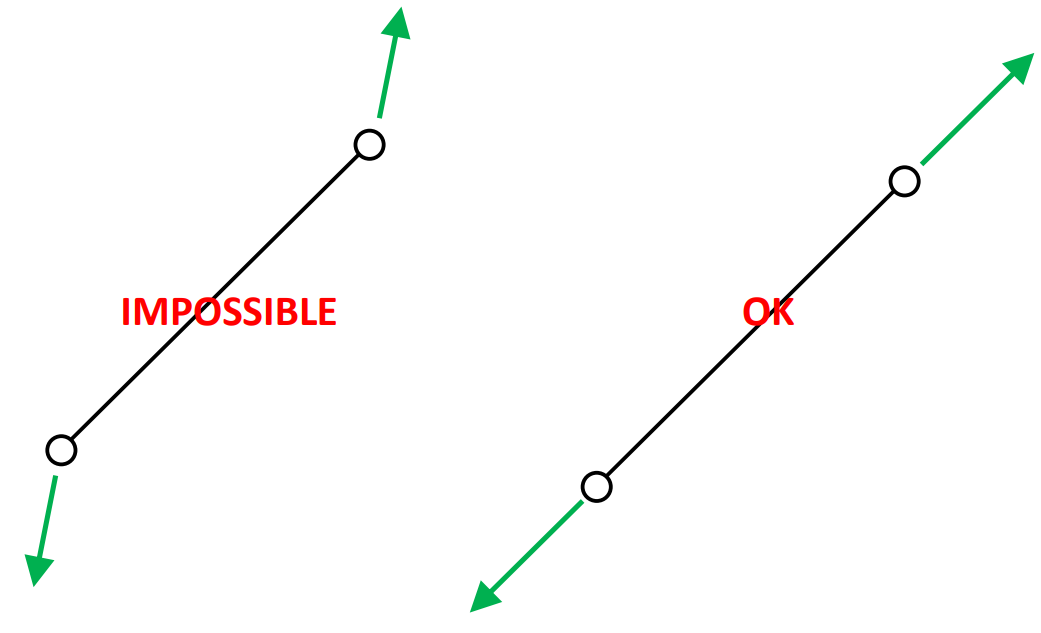
\includegraphics[width=0.5\textwidth]{images/Treillis01.PNG} \end{center}

\begin{itemize}

    \item b = nb de barres
    \item n = nb de noeuds
    \item r = nb de réactions extérieures

\end{itemize}

Le treillis est isostatique si: 2 n = b + r.

Un treillis peut être isostatique sans être stable:

\begin{center} 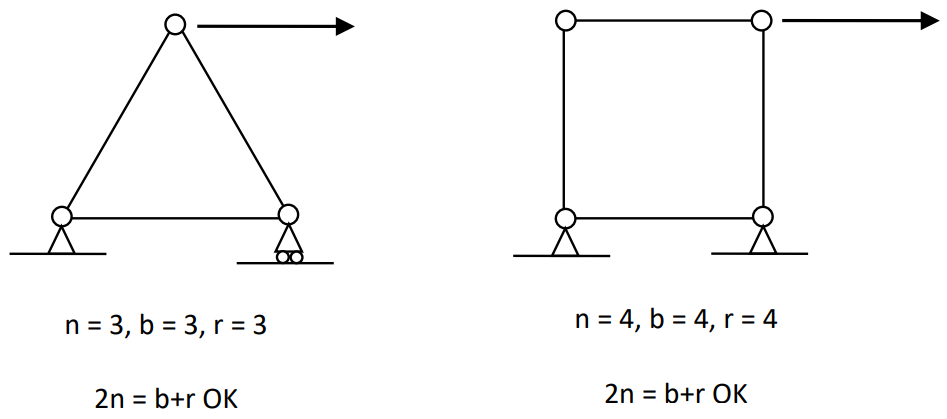
\includegraphics[width=0.5\textwidth]{images/Treillis02.PNG} \end{center}





\subsection{Résolution}





Pour résoudre le treillis,
\begin{enumerate}

    \item Si possible, on calcule les forces de réaction.
    \item On identifie les barres où les efforts sont nuls.
    \item On choisit une des deux méthodes : la méthode des noeuds ou la méthode de Ritter. La méthode des noeuds n'est pas toujours applicable, et on préfère celle de Ritter quand il n'y a pas beaucoup de forces à calculer.

\end{enumerate}

Méthode de Ritter:

\begin{center} 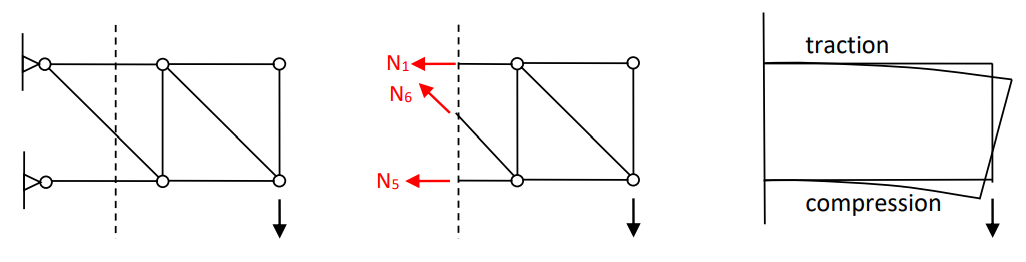
\includegraphics[width=0.85\textwidth]{images/Treillis03.PNG} \end{center}

On utilise les 3 équations d'équilibre Pour déterminer les efforts internes.

Méthode des noeuds:

\begin{center} 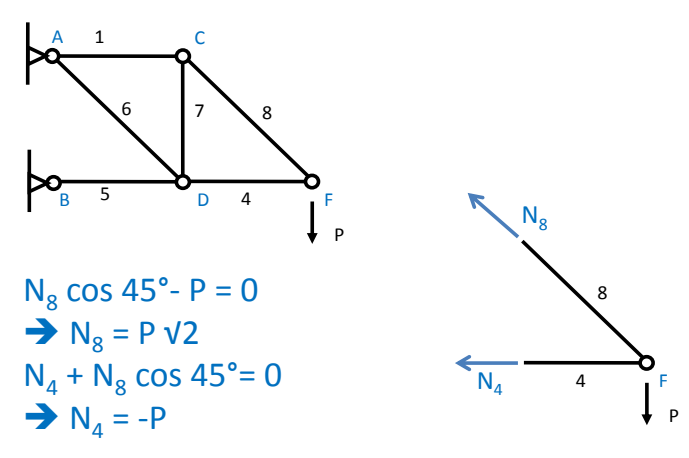
\includegraphics[width=0.48\textwidth]{images/Treillis04.PNG} 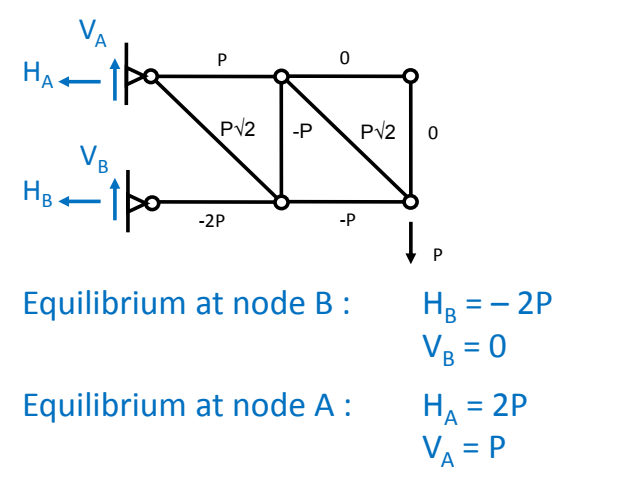
\includegraphics[width=0.48\textwidth]{images/Treillis05.PNG} \end{center}










\section{Statique \& MNT}





Une poutre peut reposer sur les supports suivants:

\begin{center} 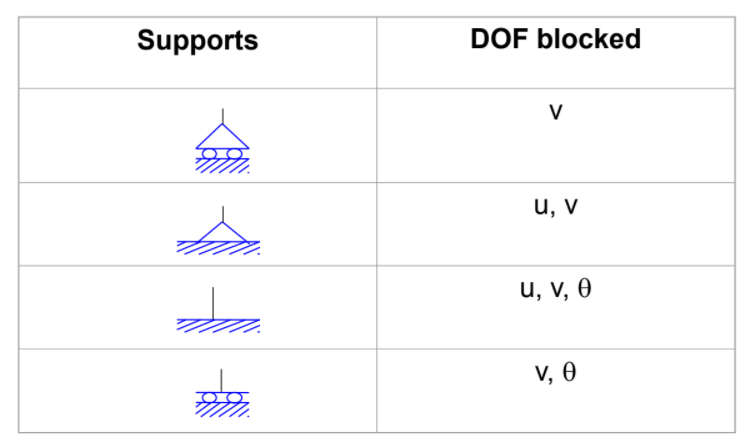
\includegraphics[width=0.5\textwidth]{images/Statique01.PNG} \end{center}





\subsection{Convention de Signes}





Dans une coupe, on dessine les forces internes ainsi : 

\begin{center} 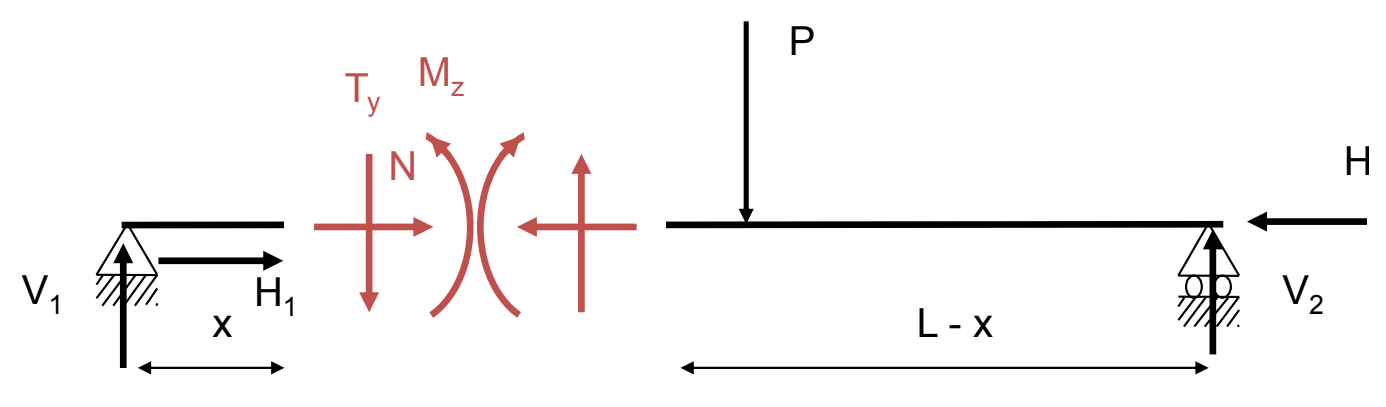
\includegraphics[width=0.65\textwidth]{images/MNT01.PNG} \end{center}

Cependant, on utilise la convention de signes suivante : $ N > 0 $ en \textbf{traction}, $ M > 0 $ si la \textbf{fibre de référence} est en \textbf{traction} et : $ T > 0 $ lorsqu'il fait \textbf{tourner} la poutre dans le \textbf{sens horaire}. \\
Quand on calcule le moment, il faut aussi dessiner une fourche qui indique la courbure de la poutre.





\subsection{Diagrammes de Base}





\begin{center} \begin{tabular}{c|c} \begin{tikzpicture}

\draw[support] (0,0);

\draw[rouleau] (6,0);

\draw[-, thick] (0,0) -- (6,0);

% force
\draw[-] (0,0.8) -- node[anchor=south]{p} (6,0.8);
\foreach \x in {0,...,6}
    \draw[->] (\x,0.8) -- (\x,0);

\draw[<->] (0,-1) -- node[anchor=south]{L} (6,-1);

% T
\draw[-, thick] (0,-2.5) node[anchor=east]{\textbf{T}} -- (6,-2.5);
\draw[-] (0,-2.5) -- (0,-1.5) node[anchor=east]{$ p L / 2 $};
\draw[-] (6,-2.5) -- (6,-3.5) node[anchor=west]{$ - p L / 2 $};
\draw[-] (0,-1.5) -- (6,-3.5);
\node [] at (0.7,-2.1) {\textbf{+}};
\node [] at (5.3,-2.9) {\textbf{-}};

% M
\draw[-, thick] (0,-4) node[anchor=east]{\textbf{M}} -- (6,-4);
\draw  plot[smooth, tension=.7] coordinates {(0,-4) (3,-5) (6,-4)};
\node[anchor=north] at (3,-5) {$ p L^2 / 8 $};

\draw[fourche] (3,-4.25);

\end{tikzpicture}
& %%%%%%%%%%%%%%%%%%%%%%%%%%%%%%%%%%%%%%%%%%%%%%%%%%%%%%%%%%%%%%%%%%%%%%%%%%%%%%%%%%%%%%%
\begin{tikzpicture}

\draw[support] (0,0);
\draw[rouleau] (6,0);
\draw[-, thick] (0,0) -- (6,0);

% force
\draw[-] (0,0) -- (6,0.8) node[anchor=south]{p};
\foreach \x in {1,...,6}
    \draw[->] (\x, 0.8/6*\x ) -- (\x,0);

\draw[<->] (0,-1) -- node[anchor=south]{L} (6,-1);

% T
\draw[-, thick] (0,-2.5) node[anchor=east]{\textbf{T}} -- (6,-2.5);
\draw[-] (0,-2.5) -- (0,{2/3 - 2.5}) node[anchor=east]{$ p L / 6 $};
\draw[-] (6,-2.5) -- (6,{2/3 - 4.5}) node[anchor=west]{$ - 2 p L / 6 $};

\draw[color=black, domain=0:6] plot (\x,{2/3 - \x^2 / 18 - 2.5}){};

\node [] at (0.5,-2.2) {\textbf{+}};
\node [] at (5.3,-2.9) {\textbf{-}};

% M
\draw[-, thick] (0,-4) node[anchor=east]{\textbf{M}} -- (6,-4);

\draw[color=black, domain=0:6] plot (\x,{-2/3 * \x + \x^3 / 54 - 4}){};

\node[anchor=north] at (3.5,-5) {$ M_{\text{max}} $};

\draw[fourche] (3.5,-4.2);

\end{tikzpicture} \end{tabular}

%%%%%%%%%%%%%%%%%%%%%%%%%%%%%%

\begin{tabular}{c|c} \begin{tikzpicture}

\draw[support] (0,0);

\draw[rouleau] (6,0);

\draw[-, thick] (0,0) -- (6,0);

% force
\draw[->] (3,0.8) node[anchor=east]{P} -- (3,0);

\draw[<->] (0,-1) -- node[anchor=south]{L} (6,-1);

% T
\draw[-] (0,-1.5) -- (3,-1.5); \draw[-] (3,-3.5) -- (6,-3.5);
\draw[-] (3,-1.5) -- (3,-3.5);
\draw[-, thick] (0,-2.5) node[anchor=east]{\textbf{T}} -- (6,-2.5);
\draw[-] (0,-2.5) -- (0,-1.5) node[anchor=east]{$ P / 2 $};
\draw[-] (6,-2.5) -- (6,-3.5) node[anchor=west]{$ - P / 2 $};
\node [] at (1.5,-2) {\textbf{+}};
\node [] at (4.5,-2.9) {\textbf{-}};

% M
\draw[-, thick] (0,-4) node[anchor=east]{\textbf{M}} -- (6,-4);
\draw (0,-4) -- (3,-5) -- (6,-4);
\node[anchor=north] at (3,-5) {$ P L /4 $};

\draw[fourche] (3,-4.25);

\end{tikzpicture}
& %%%%%%%%%%%%%%%%%%%%%%%%%%%%%%%%%%%%%%%%%%%%%%%%%%%%%%%%%%%%%%%%%%%%%%%%%%%%%%%%%%%%%%%
\begin{tikzpicture}

\draw[support] (0,0);
\draw[rouleau] (6,0);
\draw[-, thick] (0,0) -- (6,0);

% moment
\draw[->, thick] (3,-0.5) arc (-80:95:0.6); \node[] at (3.7,0.4) {M};

\draw[<->] (0,-1) -- node[anchor=south]{L} (6,-1);

% T
\draw[-] (0,-1.5) -- (6,-1.5);
\draw[-, thick] (0,-2.5) node[anchor=east]{\textbf{T}} -- (6,-2.5);
\draw[-] (0,-2.5) -- (0,-1.5) node[anchor=east]{$ M / L $};
\draw[-] (6,-2.5) -- (6,-1.5);
\node [] at (3,-2) {\textbf{+}};

% M
\draw[-, thick] (0,-4) node[anchor=east]{\textbf{M}} -- (6,-4);
\draw (0,-4) -- (3,-5) node[anchor=north]{$ M / 2 $} -- (3,-4);
\draw (3,-4) -- (3,-3) node[anchor=east]{$ - M / 2 $} -- (6,-4);

% fourches
\draw[fourche] (2.5,-4.25);
\coordinate (up) at (3.5,-3.3);
\draw (up) -- ($ (up) + (0,-0.5)$);
\draw  plot[smooth, tension=.7] coordinates {($(up) + (-0.3,-0.4)$) ($(up) + (0,-0.2)$) ($(up) + (0.3,-0.4)$)};

\end{tikzpicture}

\\ \hline %%%%%%%%%%%%%%%%%%%%%%%%%%%%%%%%%%%%%%

\begin{tikzpicture}

\draw[-] (0,0.5) -- (0,-0.5);
\fill[pattern=north east lines] (0,0.5) -- (-0.35,0.5) -- (-0.35,-0.5) -- (0,-0.5);

\draw[-, thick] (0,0) -- (6,0);

% force
\draw[->] (6,0.8) node[anchor=east]{P} -- (6,0);

\draw[<->] (0,-1) -- node[anchor=south]{L} (6,-1);

% T
\draw[-] (0,-1.5) -- (6,-1.5);
\draw[-, thick] (0,-2.5) node[anchor=east]{\textbf{T}} -- (6,-2.5);
\draw[-] (0,-2.5) -- (0,-1.5) node[anchor=east]{$ P $};
\draw[-] (6,-2.5) -- (6,-1.5);
\node [] at (3,-2) {\textbf{+}};

% M
\draw[-, thick] (0,-4) node[anchor=east]{\textbf{M}} -- (6,-4);
\draw (0,-4) -- (0,-5.5) node[anchor=north]{$ - P L $} -- (6,-4);

% fourche
\coordinate (up) at (1.5,-4.3);
\draw (up) -- ($ (up) + (0,-0.5)$);
\draw  plot[smooth, tension=.7] coordinates {($(up) + (-0.3,-0.4)$) ($(up) + (0,-0.2)$) ($(up) + (0.3,-0.4)$)};

\end{tikzpicture}
& %%%%%%%%%%%%%%%%%%%%%%%%%%%%%%%%%%%%%%%%%%%%%%%%%%%%%%%%%%%%%%%%%%%%%%%%%%%%%%%%%%%%%%%
\begin{tikzpicture}

\draw[-] (0,0.5) -- (0,-0.5);
\fill[pattern=north east lines] (0,0.5) -- (-0.35,0.5) -- (-0.35,-0.5) -- (0,-0.5);

\draw[-, thick] (0,0) -- (6,0);

% force
\draw[-] (0,0.8) -- node[anchor=south]{p} (6,0.8);
\foreach \x in {0,...,6}
    \draw[->] (\x,0.8) -- (\x,0);

\draw[<->] (0,-1) -- node[anchor=south]{L} (6,-1);

% T
\draw[-] (0,-1.5) -- (6,-2.5);
\draw[-, thick] (0,-2.5) node[anchor=east]{\textbf{T}} -- (6,-2.5);
\draw[-] (0,-2.5) -- (0,-1.5) node[anchor=east]{$ p L $};
\node [] at (1,-2) {\textbf{+}};

% M
\draw[-, thick] (0,-4) node[anchor=east]{\textbf{M}} -- (6,-4);
\draw[color=black, domain=0:6] plot (\x,{- (\x-6)^2 / 24 - 4}){};
\draw (0,-4) -- (0,-5.5) node[anchor=north]{$ - p L^2 / 2 $};

% fourche
\coordinate (up) at (1,-4.3);
\draw (up) -- ($ (up) + (0,-0.5)$);
\draw  plot[smooth, tension=.7] coordinates {($(up) + (-0.3,-0.4)$) ($(up) + (0,-0.2)$) ($(up) + (0.3,-0.4)$)};

\end{tikzpicture}

\\ \hline %%%%%%%%%%%%%%%%%%%%%%%%%%%%%%

\begin{tikzpicture}

\draw[support] (0,0);
\draw[rouleau] (6,0);
\draw[-, thick] (0,0) -- (6,0);

% moment
\draw[->, thick] (6.2,-0.8) arc (-80:95:0.6); \node[] at (7,0) {M};

\draw[<->] (0,-1) -- node[anchor=south]{L} (6,-1);

% T
\draw[-] (0,-1.5) -- (6,-1.5);
\draw[-, thick] (0,-2.5) node[anchor=east]{\textbf{T}} -- (6,-2.5);
\draw[-] (0,-2.5) -- (0,-1.5) node[anchor=east]{$ M / L $};
\draw[-] (6,-2.5) -- (6,-1.5);
\node [] at (3,-2) {\textbf{+}};

% M
\draw[-, thick] (0,-4) node[anchor=east]{\textbf{M}} -- (6,-4);
\draw (0,-4) -- (6,-5.5) node[anchor=north]{$ M $} -- (6,-4);

\draw[fourche] (4.5,-4.25);

\end{tikzpicture}
& %%%%%%%%%%%%%%%%%%%%%%%%%%%%%%%%%%%%%%%%%%%%%%%%%%%%%%%%%%%%%%%%%%%%%%%%%%%%%%%%%%%%%%%
\begin{tikzpicture}

\draw[support] (0,0);
\draw[rouleau] (6,0);
\draw[-, thick] (0,0) -- (6,0);

% moment
\draw[->, thick] (6.2,-0.8) arc (-80:95:0.6); \node[] at (7,0) {M};
\draw[->, thick] (-0.2,-0.8) arc (260:85:0.6); \node[] at (-1,0) {M};

\draw[<->] (0,-1) -- node[anchor=south]{L} (6,-1);

% T
\draw[-, thick] (0,-2.5) node[anchor=east]{\textbf{T}} -- (6,-2.5);
\node [] at (3,-2) {$ T = 0 $};

% M
\draw[-, thick] (0,-4) node[anchor=east]{\textbf{M}} -- (6,-4);
\draw (0,-4) -- (0,-5.5) -- node[anchor=north]{$ M $} (6,-5.5) -- (6,-4);

\draw[fourche] (3,-4.5);

\end{tikzpicture} \end{tabular} \end{center}





\subsection{Exemple Résolution MNT}





Examen \big[2010-2011 S2 Q1\big]: pour la structure ci-dessous ($ M = 16 \; kN m $), on demande de:
\begin{enumerate}
    \item Vérifier l’isostaticité
    \item Calculer les réactions d’appuis et les réactions internes en C ;
    \item Établir l’expression analytique des MNT ;
    \item Tracer soigneusement ces diagrammes en indiquant les valeurs caractéristiques.
\end{enumerate}

\begin{center} 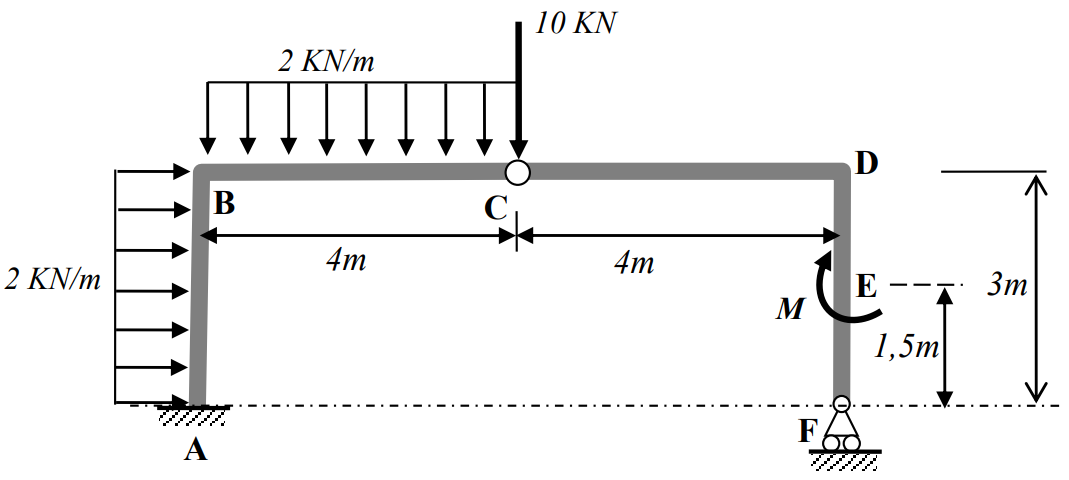
\includegraphics[width=0.6\textwidth]{images/MNT02.PNG} \end{center}



\textbf{ISOSTATICITÉ}: Il y a 4 inconnues (3 en A, 1 en F) et 3 relations d'équilibre. La rotule (en C) ajoute 2 inconnues et 3 équations. Étant donné qu'on a au total 6 équations pour 6 inconnues, la structure est bien isostatique.



\begin{tabular}{p{8cm}p{6cm}}
Équilibre à droite:
\begin{itemize}
    \item \textbf{H}: $ H_C = 0 $
    \item \textbf{M}: $ 4 V_F - 16 = 0 \implies V_F = 4 \; kN $
    \item \textbf{V}: $ V_C = - 4 \; kN $
\end{itemize}
&
Équilibre à gauche:
\begin{itemize}
    \item \textbf{H}: $ H_A = - 6 \; kN $
    \item \textbf{V}: $ V_A = 14 \; kN $
    \item \textbf{M}: $ M_A = - 49 \; kN m $
\end{itemize}
\end{tabular}

\begin{tabular}{p{5cm}p{5cm}p{5cm}}

Plage AB: & Plage BC: & Plage CD: \\
\begin{itemize}
    \item \textbf{N}: $ N = - 14 \; kN $
    \item \textbf{T}: $ T = - 2 x + 6 $
    \item \textbf{M}: $ M = -49 - x^2 + 6 x $
\end{itemize}
&
\begin{itemize}
    \item \textbf{N}: $ N = 0 $
    \item \textbf{T}: $ T = 2 x + 6 $
    \item \textbf{M}: $ M = - x^2 - 6 x $
\end{itemize}
&
\begin{itemize}
    \item \textbf{N}: $ N = 0 $
    \item \textbf{T}: $ T = - 4 \; kN $
    \item \textbf{M}: $ M = - 4 x $
\end{itemize}
\\
Plage FE: & Plage ED: & \\
\begin{itemize}
    \item \textbf{N}: $ N = N = - 4 \; kN $
    \item \textbf{T}: $ T = 0 $
    \item \textbf{M}: $ M = 0 $
\end{itemize}
&
\begin{itemize}
    \item \textbf{N}: $ N = - 4 \; kN $
    \item \textbf{T}: $ T = 0 $
    \item \textbf{M}: $ M = 16 \; kN m $
\end{itemize}
\end{tabular}

\begin{center}
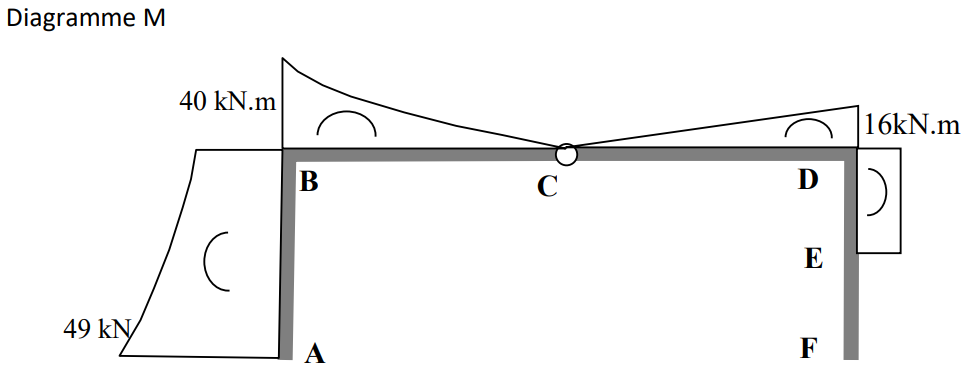
\includegraphics[width=0.48\textwidth]{images/MNT03.PNG}
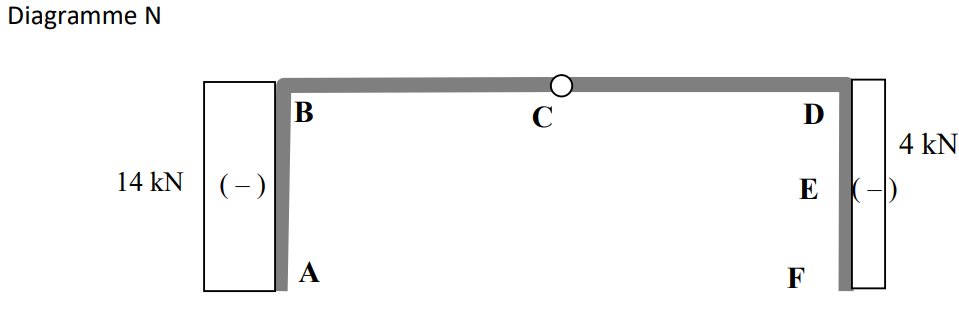
\includegraphics[width=0.48\textwidth]{images/MNT04.PNG}
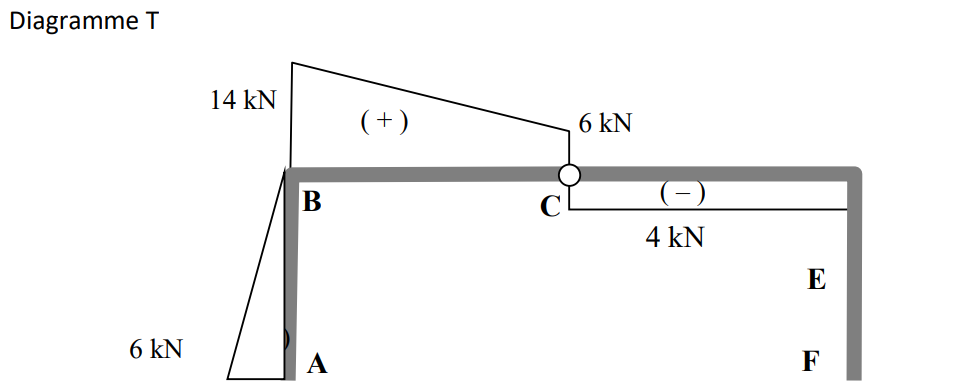
\includegraphics[width=0.48\textwidth]{images/MNT05.PNG}
\end{center}









\section{Calcul de Flèches}





La courbure de la poutre est donnée par : $\displaystyle \mathcal{X} = \frac{M}{E \; I} $. La relation entre la courbure ($ \mathcal{X} $) et les déplacements verticaux ($ \nu $) est donnée par : 
\[ \mathcal{X} = - \frac{d^2 \nu}{d x^2} \implies \frac{d^2 \nu}{d x^2} = - \frac{M}{E \; I} \]
Le problème est que quand on veut connaître le déplacement vertical à partir du moment, on obtient 2 constantes d'intégration à déterminer.





\subsection{Exemple - Base}





\begin{tikzpicture}

\draw[-] (0,0.5) -- (0,-0.5);
\fill[pattern=north east lines] (0,0.5) -- (-0.35,0.5) -- (-0.35,-0.5) -- (0,-0.5);

\draw[-, thick] (0,0) -- (6,0);

% force
\draw[->] (6,0.8) node[anchor=east]{P} -- (6,0);

\draw[<->] (0,-1) -- node[anchor=south]{L} (6,-1);
\draw[|->] (6,-0.5) -- node[anchor=south]{$ x $} (4.5,-0.5);

% M
\draw[-, thick] (0,-2) node[anchor=east]{\textbf{M}} -- (6,-2);
\draw (0,-2) -- (0,-3.5) node[anchor=north]{$ - P L $} -- (6,-2);

% fourche
\coordinate (up) at (1.5,-2.3);
\draw (up) -- ($ (up) + (0,-0.5)$);
\draw  plot[smooth, tension=.7] coordinates {($(up) + (-0.3,-0.4)$) ($(up) + (0,-0.2)$) ($(up) + (0.3,-0.4)$)};

% texte
\node [xshift=7.5cm, yshift=1cm, anchor=north west] {$\displaystyle M = - P x \implies \frac{d^2 \nu}{d x^2} = \frac{P x}{E \; I} $};
\node [xshift=7.5cm, yshift=0cm, anchor=north west] {$\displaystyle \frac{d \nu}{d x} = \frac{P}{2 E I} x^2 + C_1 $};
\node [xshift=7.5cm, yshift=-1cm, anchor=north west] {$\displaystyle \nu = \frac{P}{6 E I} x^3 + C_1 x + C_2 $};

\node [xshift=6.5cm, yshift=-2.5cm, anchor=north west] {En $ x = L $:};
\node [xshift=7cm, yshift=-3cm, anchor=north west] {$\displaystyle \frac{P}{2 E I} L^2 + C_1 = 0 \implies C_1 = - \frac{P L^2}{2 E I} $};
\node [xshift=7cm, yshift=-4cm, anchor=north west] {$\displaystyle \frac{P}{6 E I} L^3 - \frac{P L^2}{2 E I} L + C_2 = 0 \implies C_2 = \frac{P L^3}{3 E I} $};



% poutre pliée
\draw[-] (0,-4.5) -- (0,-5.5);
\fill[pattern=north east lines] (0,-4.5) -- (-0.35,-4.5) -- (-0.35,-5.5) -- (0,-5.5);
\draw[-, thick] (0,-5) -- (6,-5);
\draw[color=black, domain=0:6, thick, dashed] plot (\x,{- (\x)^2 / 24 - 5}){};
\draw[<->] (6,-5.1) -- node[anchor=west]{$\displaystyle \nu = \frac{P L^3}{3 E I} $} (6,-6.4);

\end{tikzpicture}





\subsection{Cas de Base}





\begin{center} \begin{tabular}{|c|c|c || c|c|c|} \hline &&&&& \\
Mode de Sollicitation & $ \phi_A $ & $ f $ & Mode de Sollicitation & $ \phi_A $ & $ f $ \\ &&&&& \\ \hline

\begin{tikzpicture}
\draw[-] (0,0.25) -- (0,-0.25);
\fill[pattern=north east lines] (0,0.25) -- (-0.35,0.25) -- (-0.35,-0.25) -- (0,-0.25);
\draw[-, thick] (0,0) -- (3,0) node[anchor=north]{A};
% force
\draw[->, thick] (3.2,-0.3) arc (-80:95:0.3); \node[anchor=east] at (4,0) {M};
\end{tikzpicture}
& 
\begin{tikzpicture} \node[yshift=-0.5cm]{}; \node[]{$\displaystyle - \frac{M L}{E I} $}; \end{tikzpicture}
&
\begin{tikzpicture} \node[yshift=-0.5cm]{}; \node[]{$\displaystyle - \frac{M L^2}{2 E I} $}; \end{tikzpicture}

&

\begin{tikzpicture}
\draw[-] (0,0.25) -- (0,-0.25);
\fill[pattern=north east lines] (0,0.25) -- (-0.35,0.25) -- (-0.35,-0.25) -- (0,-0.25);
\draw[-, thick] (0,0) -- (3,0) node[anchor=north]{A};
% force
\draw (0,0.5) -- node[anchor=south]{p} (3,0.5);
\foreach \x in {0,...,6}
    \draw[->] (\x/2,0.5) -- (\x/2,0);
\end{tikzpicture}
& 
\begin{tikzpicture} \node[yshift=-0.5cm]{}; \node[]{$\displaystyle \frac{p L^3}{6 E I} $}; \end{tikzpicture}
&
\begin{tikzpicture} \node[yshift=-0.5cm]{}; \node[]{$\displaystyle \frac{p L^4}{8 E I} $}; \end{tikzpicture}

\\ \hline

\begin{tikzpicture}
\draw[-] (0,0.25) -- (0,-0.25);
\fill[pattern=north east lines] (0,0.25) -- (-0.35,0.25) -- (-0.35,-0.25) -- (0,-0.25);
\draw[-, thick] (0,0) -- (3,0) node[anchor=north]{A};
% force
\draw[->] (3,0.5) node[anchor=south]{P} -- (3,0);
\draw[<->] (0,-0.6) -- node[anchor=south]{L} (3,-0.6);
\node[anchor=east] at (4,0) {};
\end{tikzpicture}
& 
\begin{tikzpicture} \node[yshift=-0.5cm]{}; \node[]{$\displaystyle \frac{P L^2}{2 E I} $}; \end{tikzpicture}
&
\begin{tikzpicture} \node[yshift=-0.5cm]{}; \node[]{$\displaystyle \frac{P L^3}{3 E I} $}; \end{tikzpicture}

&

\begin{tikzpicture}
\draw[-] (0,0.25) -- (0,-0.25);
\fill[pattern=north east lines] (0,0.25) -- (-0.35,0.25) -- (-0.35,-0.25) -- (0,-0.25);
\draw[-, thick] (0,0) -- (3,0) node[anchor=north]{A};
% force
\draw (0,0.5) node[anchor=south]{p} -- (3,0);
\foreach \x in {0,...,5}
    \draw[->] (\x/2,-0.5/6*\x+0.5) -- (\x/2,0);
\draw[<->] (0,-0.6) -- node[anchor=south]{L} (3,-0.6);
\end{tikzpicture}
& 
\begin{tikzpicture} \node[yshift=-0.5cm]{}; \node[]{$\displaystyle \frac{P L^2}{12 E I} $}; \end{tikzpicture}
&
\begin{tikzpicture} \node[yshift=-0.5cm]{}; \node[]{$\displaystyle \frac{P L^3}{15 E I} $}; \end{tikzpicture}

\\ \hline

\end{tabular} \end{center}





\begin{center} \begin{tabular}{|c|c|c|c|} \hline

Mode de Sollicitation & $ M_{\text{max}} $ & $ \phi $ & $ f $ \\ \hline

\begin{tikzpicture}[]
\draw[petitsupport] (0,0) node[anchor=south]{A};
\draw[petitrouleau] (3,0) node[anchor=south]{B};
\draw[-, thick] (0,0) -- (3,0);
\draw[->, thick] (3.2,-0.3) arc (-80:95:0.3); \node[anchor=east] at (4,0) {M};
\end{tikzpicture}
&
\begin{tikzpicture} \node[yshift=-0.25cm]{}; \node[]{$ M $}; \end{tikzpicture}
&
\begin{tikzpicture} \node[yshift=-0.25cm]{}; \node[]{$\displaystyle \phi_A = \frac{M L}{6 E I} \; ; \; \phi_B = - \frac{M L}{3 E I} $}; \end{tikzpicture}
&
\begin{tikzpicture} \node[yshift=-0.25cm]{}; \node[]{$\displaystyle \frac{M L^2}{16 E I} $}; \end{tikzpicture}

\\ \hline

\begin{tikzpicture}[]
\draw[petitsupport] (0,0) node[anchor=south]{A};
\draw[petitrouleau] (3,0) node[anchor=south]{B};
\draw[-, thick] (0,0) -- (3,0);
\draw[->] (1.5,0.5) node[anchor=south]{P} -- (1.5,0);
\end{tikzpicture}
&
\begin{tikzpicture} \node[yshift=-0.5cm]{}; \node[]{$\displaystyle \frac{P L}{4} $}; \end{tikzpicture}
&
\begin{tikzpicture} \node[yshift=-0.5cm]{}; \node[]{$\displaystyle \pm \frac{P L^2}{16 E I} $}; \end{tikzpicture}
&
\begin{tikzpicture} \node[yshift=-0.5cm]{}; \node[]{$\displaystyle \frac{P L^3}{48 E I} $}; \end{tikzpicture}

\\ \hline

\begin{tikzpicture}[]
\draw[petitsupport] (0,0);
\draw[petitrouleau] (3,0);
\draw[-, thick] (0,0) -- (3,0);
\foreach \x in {0,...,6}:
    \draw[->] (\x/2,0.5) -- (\x/2,0);
\draw[-] (0,0.5) -- node[anchor=south]{p} (3,0.5);
\end{tikzpicture}
&
\begin{tikzpicture} \node[yshift=-0.5cm]{}; \node[]{$\displaystyle \frac{p L^2}{8} $}; \end{tikzpicture}
&
\begin{tikzpicture} \node[yshift=-0.5cm]{}; \node[]{$\displaystyle \pm \frac{p L^3}{24 E I} $}; \end{tikzpicture}
&
\begin{tikzpicture} \node[yshift=-0.5cm]{}; \node[]{$\displaystyle \frac{5 p L^4}{384 E I} $}; \end{tikzpicture}

\\ \hline

\begin{tikzpicture}[]
\draw[petitsupport] (0,0);
\draw[petitrouleau] (3,0);
\draw[-, thick] (0,0) -- (3,0);
\foreach \x in {1,...,6}:
    \draw[->] (\x/2,0.8*\x/6) -- (\x/2,0);
\draw[-] (0,0) -- node[anchor=south east]{charge totale = P} (3,0.8);
\end{tikzpicture}
&
\begin{tikzpicture} \node[yshift=-0.5cm]{}; \node[]{$\displaystyle \frac{2 P L}{9 \sqrt{3}} $}; \end{tikzpicture}
&
\begin{tikzpicture} \node[yshift=-0.5cm]{}; \node[]{$\displaystyle \phi_A = \frac{7 P L^2}{180 E I} \; ; \; \phi_B = - \frac{8 P L^2}{180 E I} $}; \end{tikzpicture}
&
\begin{tikzpicture} \node[yshift=-0.7cm]{($ x = 0,5191 $)}; \node[]{$\displaystyle 0,0130 \frac{P L^3}{E I} $}; \end{tikzpicture}

\\ \hline

\end{tabular} \end{center}

Les tableaux sont les mêmes que dans le livre aux pages 255-256.





\subsection{Résolution}





\begin{enumerate}

\item Diviser la structure en tronçons rectilignes pour ne plus avoir que des cas de base.
\item Démarrer d'un point fixe et progresser dans la structure, en considérant les autres tronçons comme indéformables.
\item Combiner les déformations.

\end{enumerate}





\subsection{Exemple}





On demande d'établir la flèche verticale et la rotation en D. On ne tient pas compte des déformations dues à la flexion. Les diagrammes MNT de la poutre sont donnés.

\begin{center}
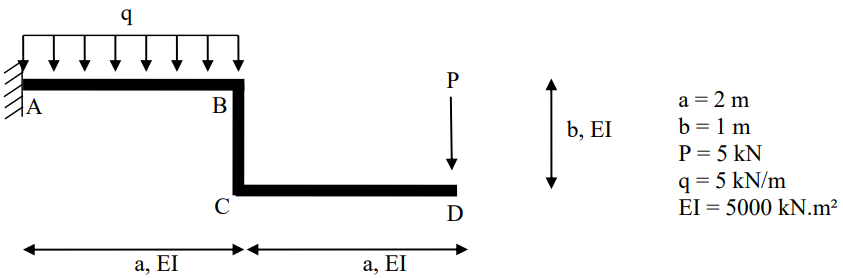
\includegraphics[width=0.75\textwidth]{images/Fleches01.PNG}
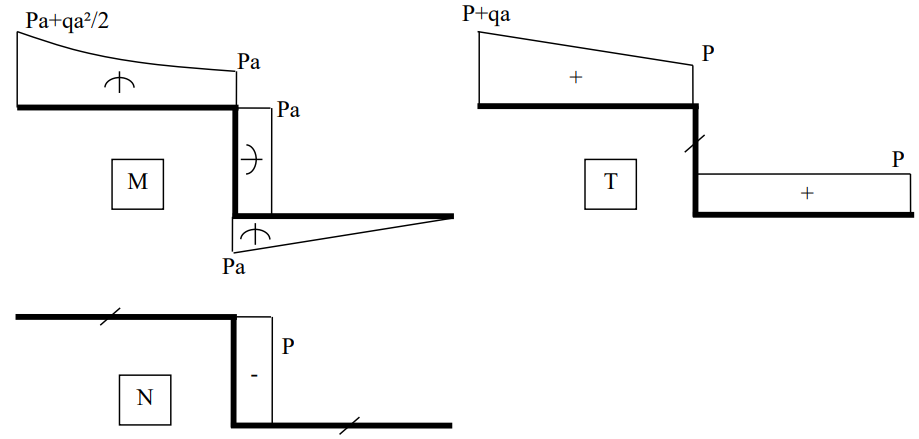
\includegraphics[width=0.75\textwidth]{images/Fleches02.PNG}
\end{center}

\begin{tabular}{p{5.5cm}p{5.5cm}p{5.5cm}}

Tronçon AB: & Tronçon BC: & Tronçon CD: \\
\begin{tikzpicture}
\draw[-] (0,0.25) -- (0,-0.25);
\fill[pattern=north east lines] (0,0.25) -- (-0.35,0.25) -- (-0.35,-0.25) -- (0,-0.25);
\draw[-, thick] (0,0) -- (3,0);
% force
\draw (0,0.5) -- node[anchor=south]{q} (3,0.5);
\foreach \x in {0,...,6}
    \draw[->] (\x/2,0.5) -- (\x/2,0);
\draw[->] (3,-0.05) -- (3,-0.5) node[anchor=north]{P};
\draw[->, thick] (3.2,-0.3) arc (-80:95:0.3); \node[anchor=east] at (4.1,0) {$ P a $};
\end{tikzpicture}
&
\begin{tikzpicture}
\draw[-, thick] (0,0) -- (0,1.5);
\draw[-, thick] (0,0) -- (3,0);
% forces
\draw[->] (0,1.55) -- (0,2) node[anchor=south]{P};
\draw[->] (3,0.5) node[anchor=south]{P} -- (3,0);
\draw[->] (0.25,1.25) arc (-60:85:0.25) node[anchor=west, xshift=0.1cm]{$ P a $};
\end{tikzpicture}
&
\begin{tikzpicture}
\draw[-, thick] (0,0) -- (3,0);
% forces
\draw[->] (3,-0.05) -- (3,-0.5) node[anchor=north]{P};
\draw[->] (0,0.05) -- (0,0.5) node[anchor=south]{P};
\draw[->] (-0.25,0.25) arc (120:275:0.25) node[anchor=east, xshift=-0.1cm]{$ P a $};
\end{tikzpicture}

\end{tabular}



\begin{tikzpicture}

\node [anchor=east] at (-1.5,0) {Tronçon AB:};

% mur
\draw[-, thick, red] (0,0.5) -- (0,-0.5);
\fill[pattern=north east lines] (0,0.5) -- (-0.35,0.5) -- (-0.35,-0.5) -- (0,-0.5);

% structure
\draw[-, thick, red] (0,0) -- (3,0);
\draw[-, thick] (3,0) -- (3,-2);
\draw[-, thick] (3,-2) -- (6,-2);

% force
\draw[-, red] (0,0.5) -- node[anchor=south]{q} (3,0.5);
\foreach \x in {0,...,6}
    \draw[->, red] (\x/2,0.5) -- (\x/2,0);
\draw[-|>, thick, red] (2.9,0.6) node[anchor=south, red]{P} -- (2.9,0);
\draw[->, thick, red] (3.2,-0.3) arc (-80:95:0.3); \node[anchor=east, red] at (4.1,0) {$ P a $};

% structure BIS
\coordinate (A) at (0,0);
\coordinate (B) at (3,-0.5);
\coordinate (C) at ($(3,-0.5) + (-110:2cm)$);
\coordinate (D) at ($(3,-0.5) + (-110:2cm) + (-20:3cm)$);
\draw[color=blue, thick, domain=0:3] plot (\x,{- 0.5 * (\x)^2 / 9}){};
\draw[color=blue, thick] (B) -- (C);
\draw[color=blue, thick] (C) -- (D);
\draw[-] ($(B) + (-0.15,-0.1) + (-200:0.2)$) -- ($(B) + (-0.15,-0.1) $) -- ($(B) + (-0.15,-0.1) + (-110:0.2)$);
\draw[-] ($(C) + (0.15,0.1) + (70:0.2)$) -- ($(C) + (0.15,0.1)$) -- ($(C) + (0.15,0.1) + (-20:0.2)$);

% mesures
\draw[dashed] (D) -- ($(D) + (1.4,0)$);
\draw[<->] (6,-2) -- node[anchor=west]{$ \nu_{D_1} $} (6,-3.4);
\draw[dashed] (D) -- ($(D) + (-20:1.5cm)$);
\draw ($ (D) + (1.3,0) $) arc (0:-20:1.3cm) node[anchor=south west]{$ \phi_1 $};
\draw[<->] (4.5,0) -- node[anchor=west]{$ f_1 $} (4.5,-0.5);

% texte
\node[xshift=5.5cm, anchor=north west, yshift=1cm]{$\displaystyle f_1 = f_q + f_P + f_M = \frac{q a^4}{8 E I} + \frac{P a^3}{3 E I} + \frac{P a \; a^2}{2 E I} $};
\node[xshift=5.5cm, anchor=north west, yshift=-0.5cm]{$\displaystyle \phi_1 = \phi_q + \phi_P + \phi_M = \frac{q a^3}{6 E I} + \frac{P a^2}{2 E I} + \frac{P a \; a}{E I} $};
\node[xshift=7cm, anchor=north west, yshift=-2cm]{$\displaystyle \nu_{D_1} = f_1 + \phi_1 a $};

\end{tikzpicture}



\begin{tikzpicture}

\node [anchor=east] at (-1,0) {Tronçon BC:};

% mur
\draw[-, thick, red] (0.5,0) -- (-0.5,0);
\fill[pattern=north east lines] (0.5,0) -- (0.5,0.35) -- (-0.5,0.35) -- (-0.5,0);

% moment
\draw[->, thick, red] (0.4,-1.6) arc (45:-135:0.8cm) node[anchor=north west, xshift=1.1cm]{$ P a $};

% structure
\draw[-, thick, red] (0,0) -- (0,-2);
\draw[-, thick] (0,-2) -- (3,-2);

% structure BIS
\coordinate (C) at (-0.5,-2);
\coordinate (D) at ($ (C) + (-20:3cm) $);
\draw[color=blue, thick, domain=0:2, rotate=-90] plot (\x,{- 0.5 * (\x)^2 / 4}){};
\draw[color=blue, thick] (C) -- (D);

% mesures
\draw[dashed] (D) -- ($(D) + (1.4,0)$);
\draw[<->] (3,-2) -- node[anchor=west]{$ \nu_{D_2} = \phi_2 a $} (3,-3);
\draw[dashed] (D) -- ($(D) + (-20:1.5cm)$);
\draw ($ (D) + (1.3,0) $) arc (0:-20:1.3cm) node[anchor=south west]{$ \phi_2 $};

% texte
\node[xshift=2.5cm, yshift=0cm, anchor=north west]{$\displaystyle \phi_2 = \frac{P a \; b}{E I} $};




\node[xshift=8.5cm]{Tronçon CD:};

\draw[-, thick] (7,-0.5) -- (7,-1.5);
\fill[pattern=north east lines] (7,-0.5) -- (6.65,-0.5) -- (6.65,-1.5) -- (7,-1.5);
\draw[-, thick] (7,-1) -- (10,-1);
\draw[color=blue, domain=0:3, thick, xshift=7cm, yshift=-1cm] plot (\x,{- 0.5 * (\x)^2 / 9}){};
\draw[<->] (10,-1) -- node[anchor=west]{$\displaystyle \nu_{D_3} $} (10,-1.5);
\coordinate (D) at (10,-1.5);
\draw[dashed] (D) -- ($(D) + (1.4,0)$);
\draw[dashed] (D) -- ($(D) + (-20:1.5cm)$);
\draw ($ (D) + (1.3,0) $) arc (0:-20:1.3cm) node[anchor=south west]{$ \phi_3 $};
\node[anchor=north west] at (7,-3) {$\displaystyle \nu_{D_3} = \frac{P a^3}{3 E I} \qquad \phi_3 = \frac{P a^2}{2 E I} $};

\end{tikzpicture}


Au final, on a :
\[ v_D = v_{D_1} + v_{D_2} + v_{D_3} = \frac{7 q a^4}{24 E I} + \frac{P a^2 b}{E I} + \frac{8 P a^3}{3 E I} \approx 3cm \]
\[ \phi_D = \phi_1 + \phi_2 + \phi_3 = \frac{q a^3}{6 E I} + \frac{P a b}{E I} + \frac{2 P a^2}{E I} \approx 0,01133 \text{ rad} = 0,649° \]





\subsection{Déplacement Dû à la Torsion}





\begin{center} 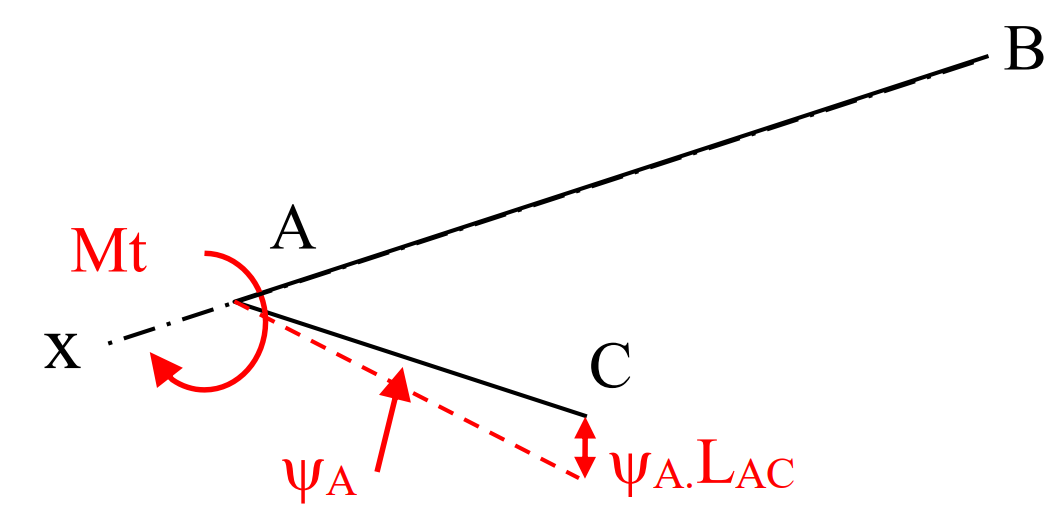
\includegraphics[width=0.5\textwidth]{images/Fleches03.PNG} \end{center}

Ici, on a une poutre qui est encastrée au point B. Le moment de torsion $ M_T $ va engendrer la rotation de la section en A. C'est une rotation d'angle $ \Uppsi_A $. Le déplacement en C vaut donc : $ \Uppsi_A L_{AC} $.











\section{Flexion - Poutre de Deux Matériaux Différents}





\subsection{Résolution}





Quand on a une poutre faîte de 2 matériaux différents, le module de Young (\emph{E}) est différent. Si il faut déterminer les contraintes dans une section, on applique la méthode suivante :
\begin{enumerate}

\item Remplacer la section réelle en une section fictive avec un seul matériau.
\item Calculer l'inertie de la nouvelle section.
\item Calculer les contraintes flexionnelles de la section fictive.
\item Re-calculer les contraintes flexionnelles pour la section réelle

\end{enumerate}





\subsection{Exemple}





\begin{enumerate}

\item Section réelle $ \implies $ Section fictive

\begin{tikzpicture}

\node[rectangle, minimum width=1.2cm, minimum height=1.7cm, draw=black, fill=black!30]{};
\node[rectangle, minimum width=1cm, minimum height=1.5cm, draw=black, pattern=north east lines, fill=white]{};
\node[rectangle, minimum width=1cm, minimum height=1.5cm, pattern=north east lines]{};

\node[rectangle, draw=black, fill=black!30, xshift=2cm, yshift=0.5cm, minimum height=0.4cm, minimum width=0.4cm]{}; \node[xshift=2.5cm, yshift=0.5cm, anchor=west]{acier};
\node[rectangle, draw=black, pattern=north east lines, xshift=2cm, yshift=-0.5cm, minimum height=0.4cm, minimum width=0.4cm]{}; \node[xshift=2.5cm, yshift=-0.5cm, anchor=west]{béton};

\node[xshift=4cm, anchor=west, yshift=0.5cm]{La poutre fléchie autour de l'axe \textbf{horizontal}.};
\node[xshift=4.5cm, anchor=west, yshift=0cm]{b = largeur béton};

% acier fictif
\coordinate (A) at (0,-2);
\node[rectangle, minimum width=1.2cm, minimum height=1.7cm, draw=black, fill=black!30] at (A) {};
\node[rectangle, minimum width=1cm, minimum height=1.5cm, draw=black, pattern=north east lines, fill=white] at (A) {};
\node[rectangle, minimum width=0.35cm, minimum height=1.6cm, fill=black!30] at (A) {};
\draw[-] ($(A) + (-0.175,0.75)$) -- ($(A) + (-0.175,-0.75)$); \draw[-] ($(A) + (0.175,0.75)$) -- ($(A) + (0.175,-0.75)$);

\node[xshift=3cm] at (A) {b' = largeur acier fictif};
\node[xshift=5cm, anchor=west] at (A) {$\displaystyle b' \; E_{\text{acier}} = b \; E_{\text{béton}} \implies b' = b \; \frac{E_{\text{béton}}}{E_{\text{acier}}} $};

\end{tikzpicture}

\item Calcul inertie de la section fictive $ \implies I' $

\item Contraintes flexionnelles : $\displaystyle \sigma' = \frac{M_y}{I'} $

\item Contraintes flexionnelles \textbf{réelles} : $\displaystyle \sigma = \sigma' \; \frac{E_{\text{béton}}}{E_{\text{acier}}} $

\end{enumerate}


Remarque: voir la Q3 de janvier 2016-2017 pour un exemple plus poussé.










\section{Déformées de Second Ordre \& Flambements}





\textbf{Définitions}:
\begin{itemize}

    \item La déformée de second ordre est la déformation finale causée par les efforts que subit la poutre en situation déformée.
    \item Le flambement est un phénomène d’instabilité qui apparaît lorsqu’une poutre est comprimée.

\end{itemize}





\begin{tikzpicture}

% structure
\draw[rouleau] (0,0);
\draw[support] (6,0);
\draw[-] (0,0) -- (6,0);

% forces
\draw[-] (0,1) -- node[anchor=south]{p} (6,1);
\foreach \x in {0,...,6}
    \draw[->] (\x,1) -- (\x,0);
\draw[->] (-1.1,0) -- (-0.1,0) node[anchor=south east]{N};

% mesure
\draw[<->] (0,-1) -- node[anchor=south]{L} (6,-1);

% texte
\node[anchor=north west] at (6.5,1) {Au 1er ordre, on a en L/2: $\displaystyle M_0 = \frac{p L^2}{8} $, et:};
\node[anchor=north west] at (9.5,0) {$\displaystyle f_0 = \frac{5 p L^4}{384 E I} $};

% space
\node[yshift=-2cm]{};

\end{tikzpicture}

La force \emph{N} engendre un moment dans la poutre qui la fait fléchir encore plus. Au final, il y a deux possibilités:
\begin{itemize}

    \item Soit il y a convergence et on a un déplacement final qui vaut: $\displaystyle f_2 = f_0 \; \frac{1}{1 - \frac{N}{N_{cr}} } $
    \item Soit il y a divergence et flambement de la poutre si: $\displaystyle N \geq N_{cr} = \frac{\pi^2 E I}{L^2_{fl}} $

\end{itemize}

Dans l'expression de: $ N_{cr} $, on a: \emph{I}, l'inertie flexionnelle de la poutre et: $ L_{fl} $, la longueur de flambement de la poutre, tel que: $ L_{fl} = L \; K $, où \emph{K} est un coefficient qui dépend des appuis de la poutre.

\begin{center} 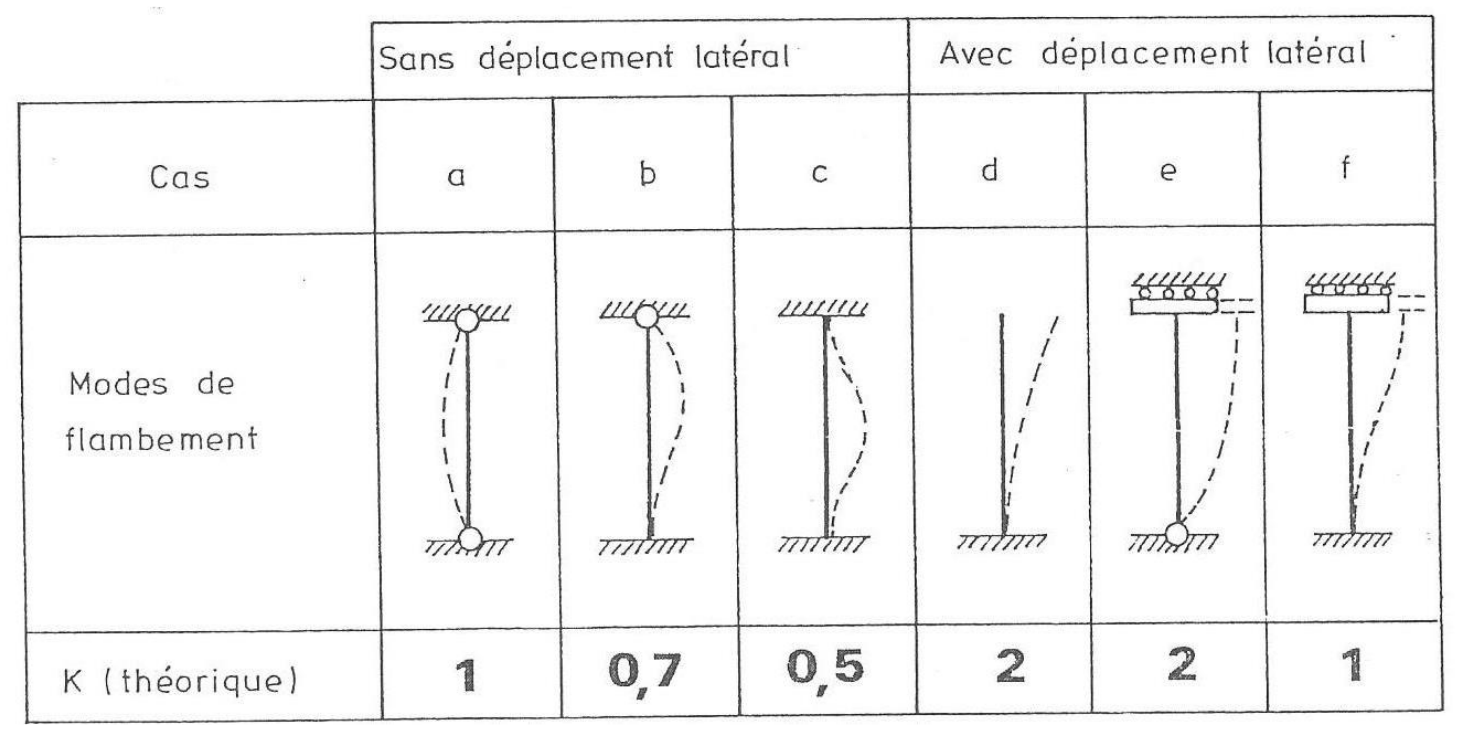
\includegraphics[width=0.85\textwidth]{images/flambement01.PNG} \end{center}

Pour retrouver la valeur du coefficient \emph{K}, on peut comprendre que la longueur de flambement est la distance entre deux points d’inflexion de la déformée de flambement de la poutre (dessinée en pointillé dans le tableau ci-dessous pour chaque cas).

\begin{center} 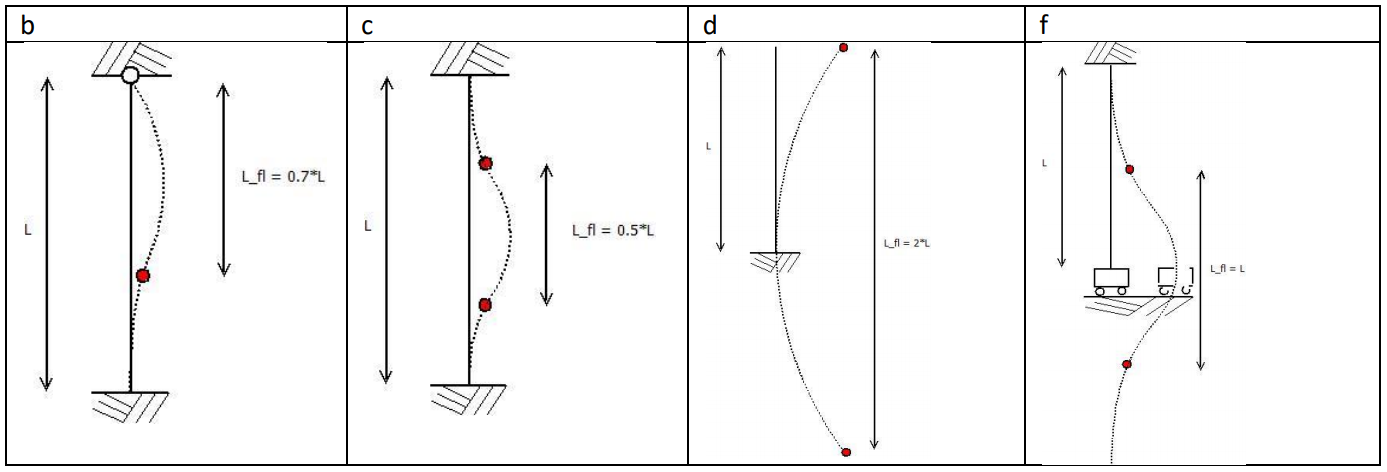
\includegraphics[width=\textwidth]{images/flambement02.PNG} \end{center}





\subsection{Exemple}





\begin{center}
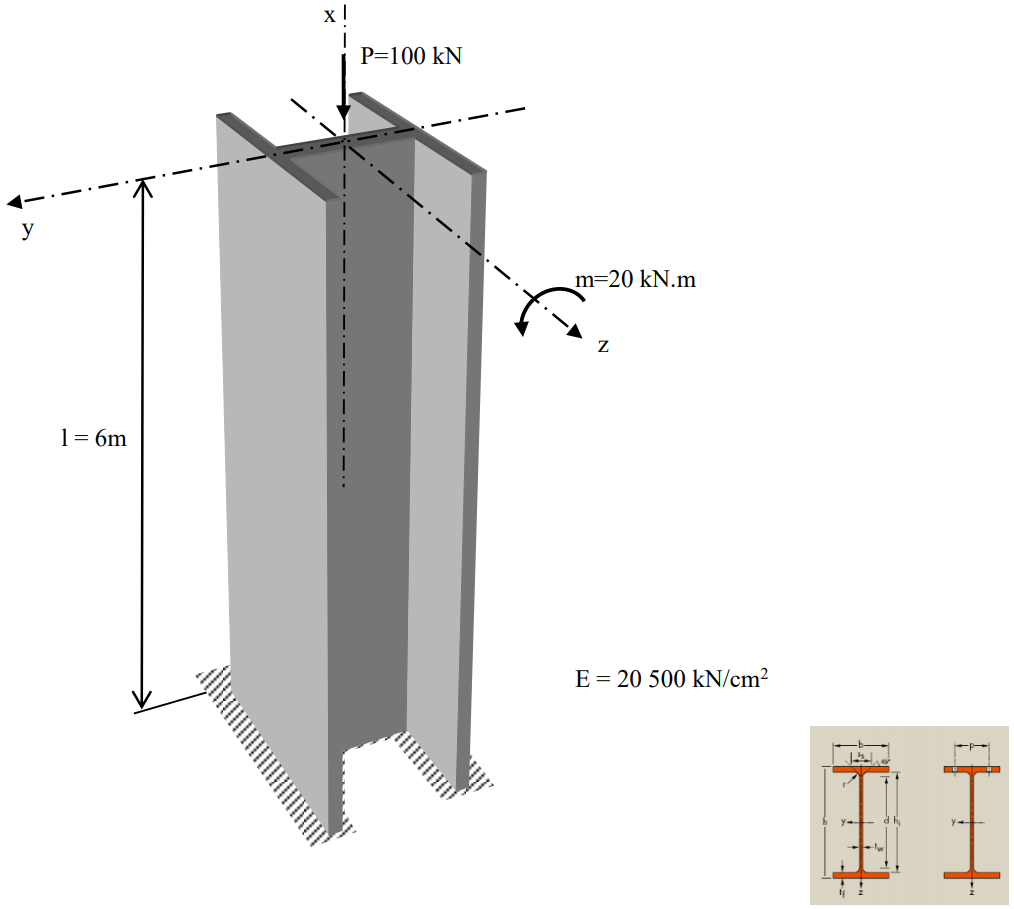
\includegraphics[width=0.75\textwidth]{images/flambement03.PNG}
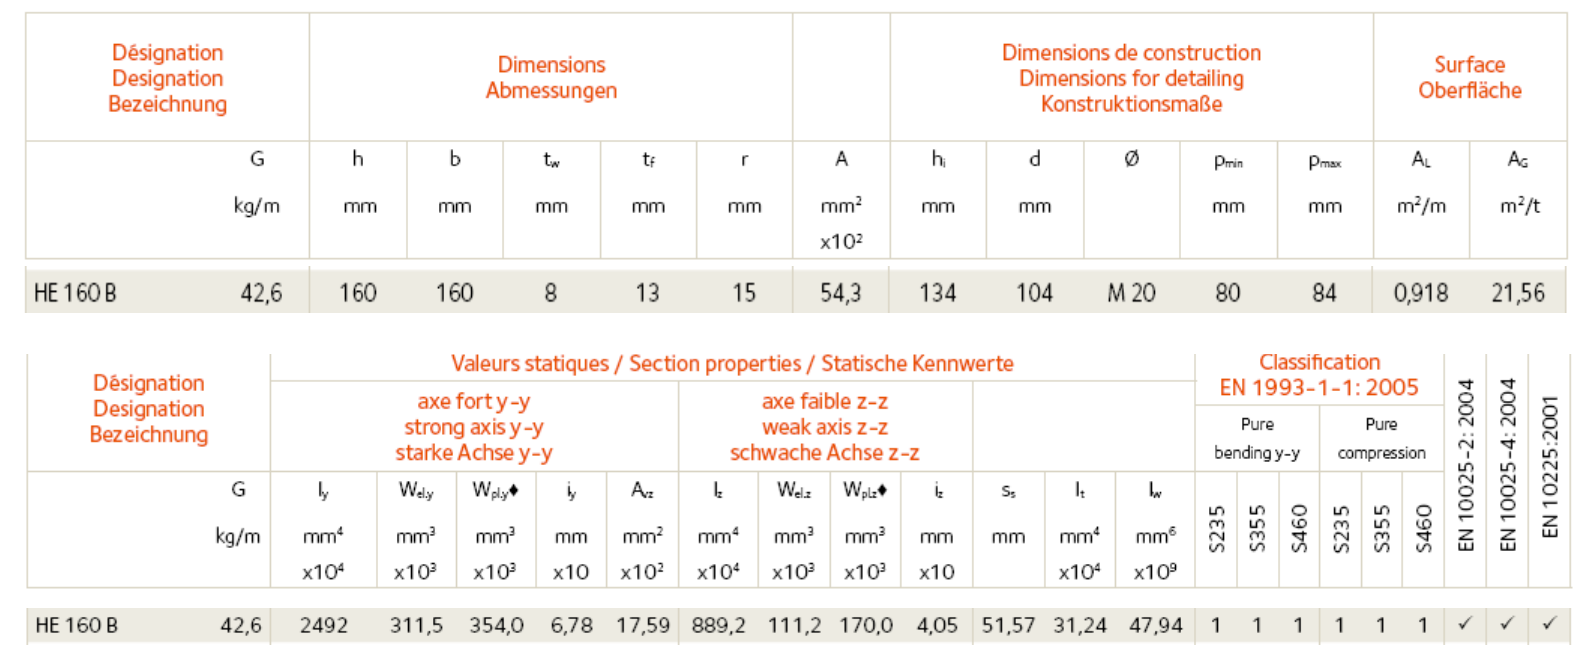
\includegraphics[width=0.75\textwidth]{images/flambement04.PNG}
\end{center}

Une poutrelle HE 160 B est encastrée verticalement dans le sol. Elle est soumise à un moment Mz = 20 kN.m et à une force axiale P=100 kN. On demande: 
\begin{enumerate}

    \item De vérifier la résistance au flambement dans les plans xy et xz ;
    \item De calculer la flèche totale (sans intégration) dans le plan xy ;
    \item De calculer le moment de flexion Mz dans la section d’encastrement ;
    \item De calculer les contraintes maximum et minimum dans cette section.

\end{enumerate}



Données: L = 6 m, E = 20500 kN/cm$^2$, A = 2492 cm$^2$, $ I_z $ = 2492 cm$^4$, $ I_y $ = 889,2 cm$^4$.





\newpage





\begin{siderules}



\[ K = 2 \implies L_{fl} = L \; K = 12 m \]

\begin{enumerate}

\item Résistance au flambement: 
\begin{itemize}
    \item Plan xy: $\displaystyle N_{cr} = \frac{\pi^2 E I_z}{(2 L)^2} = 350 \; kN > P = 100 \; kN \implies $ OK
    \item Plan xz: $\displaystyle N_{cr} = \frac{\pi^2 E I_y}{(2 L)^2} = 120 \; kN > P = 100 \; kN \implies $ OK
\end{itemize}

\item Flèche totale:
\[ f_0 = \frac{M_z L^2}{2 E I_z} = 7,047 \; cm \implies f_2 = f_0 \; \frac{1}{1 - \frac{N}{N_{cr}}} = 9,864 \; cm \]

\item Moment à l'encastrement: \\
\begin{tikzpicture}

% structure
\draw[-, thick] (-0.5,0) -- (0.5,0);
\fill[pattern=north east lines] (-0.5,0) -- (0.5,0) -- (0.5,-0.35) -- (-0.5,-0.35);
\draw[-, thick] (0,0) -- (0,3);
\draw[color=blue, thick, domain=0:3, rotate=90] plot (\x,{- (\x)^2 / 9}){};

% forces
\draw[->, blue, thick] (0.6,3) arc (180:0:0.3) node[anchor=west]{$ M_z $};
\draw[->, blue, thick] (1,4) -- node[anchor=west]{N} (1,3);

% texte
\node[xshift=5cm, yshift=2cm, anchor=north west]{$ M_2 = M_z + N \; f_2 = 2986 \; kN cm $};

\end{tikzpicture}

\item Contraintes max/min: \\
\begin{tikzpicture}

% structure
\draw[-, thick] (-0.5,0) -- (0.5,0);
\fill[pattern=north east lines] (-0.5,0) -- (0.5,0) -- (0.5,-0.35) -- (-0.5,-0.35);
\draw[-, thick] (0,0) -- (0,3);

% moment
\draw[-, green] (2,0) node[anchor=west]{$ M_2 $} -- (0.75,3) node[anchor=west]{$ M_z $};
\draw[-, green] (0,3) -- (0.75,3);
\draw[-, green] (0,0) -- (2,0);

% texte
\node[anchor=north west] at (4,3) {Les contraintes sont max/min à l'encastrement.};
\node[anchor=north west] at (4.5,2.5) {\textemdash \; $\displaystyle \sigma_N = \frac{N}{A} = \frac{- P}{A} = - 1,843 \; kN/cm^2 $};
\node[anchor=north west] at (4.5,1.5) {\textemdash \; $\displaystyle \sigma_{M_2} = \pm \frac{M_2 \; y_{\text{max}}}{I_z} = \pm 9,572 \; kN/cm^2 $};
\node[anchor=north west] at (4,0.5) {$\displaystyle \implies 
\begin{cases}
\sigma_{\text{max}} = 9,572 - 1,843 = 7,729 \; kN/cm^2 \\
\sigma_{\text{min}} = - 9,572 - 1,843 = -11,415 \; kN/cm^2
\end{cases} $};

\end{tikzpicture}

\end{enumerate}



\end{siderules}










\section{Tension - Compression}





Formulaire:
\begin{itemize}

\item $\displaystyle N = \int_A \sigma_N \; d A $
\item $\displaystyle \sigma_N = \frac{N}{A} $
\item $\displaystyle \Delta L = \int_0^L \mathcal{E} \; d x $ ($ \Delta L $ = allongement, $ \mathcal{E} $ = déformation)
\item $\displaystyle \sigma_N = E \; \mathcal{E} $ \; (E = module de Young)
\item $\displaystyle \mathcal{E} = \frac{\Delta L}{L} $
\item $ \begin{cases}
\displaystyle \mathcal{E}_x = \frac{1}{E} (\sigma_x - \nu \; \sigma_y) \\
\displaystyle \mathcal{E}_y = \frac{1}{E} (\sigma_y - \nu \; \sigma_x)
\end{cases}
\begin{cases}
\displaystyle \mathcal{E}_x = \frac{1}{E} \big( \sigma_x - \nu \; (\sigma_y + \sigma_z) \big) \\
\displaystyle \mathcal{E}_y = \frac{1}{E} \big( \sigma_y - \nu \; (\sigma_x + \sigma_z) \big) \\
\displaystyle \mathcal{E}_z = \frac{1}{E} \big( \sigma_z - \nu \; (\sigma_x + \sigma_y) \big)
\end{cases} $
\item Formule des chaudières : $\displaystyle \sigma_r = \frac{N}{e} = \frac{p \; r}{e} $, résultante : $\displaystyle P = p \; \pi r^2 $
\item Contraintes longitudinales (chaudières) : $\displaystyle \sigma_l = \frac{p \; r}{2 e} $

\end{itemize}










\section{Flexion}





\subsection{Contrainte Normale Due à la Flexion}





%% Définition
\textbf{Définition} : La flexion est la déformation d'un objet qui se traduit par une courbure. \\
La flexion résulte des moments fléchissants : $ M_y $ et  $ M_z $. Pour rappel, $\displaystyle T = \frac{d M_z}{d x} $.

\begin{center} \begin{tikzpicture}

\node () [yshift=2.5cm] {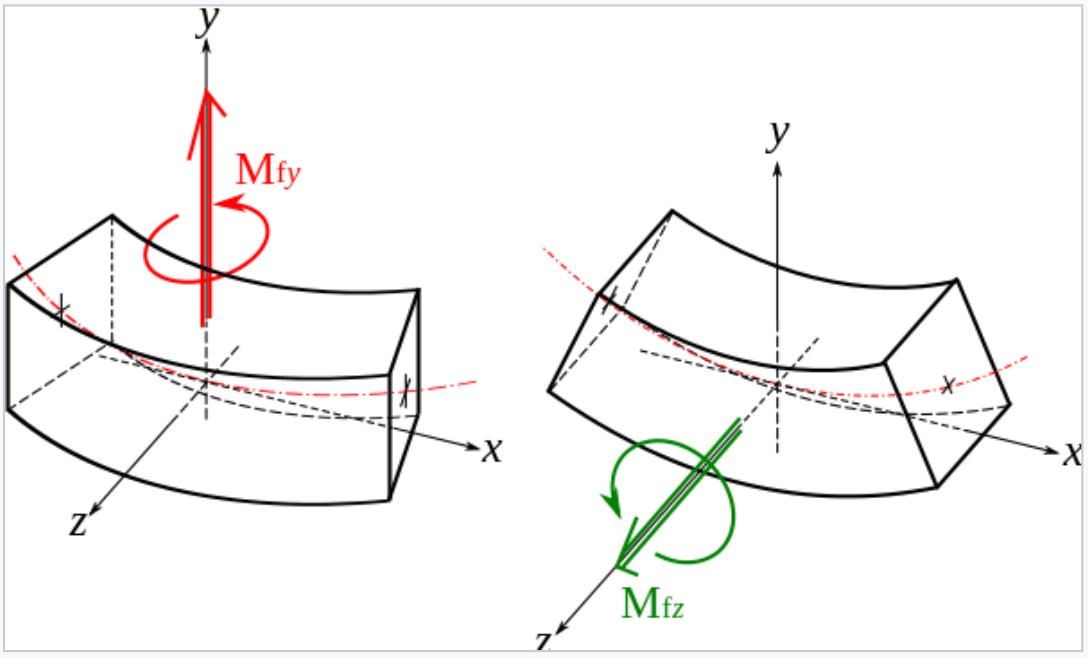
\includegraphics[width=0.50\textwidth]{images/Flexion01.PNG}};
\node () [xshift=8.5cm] {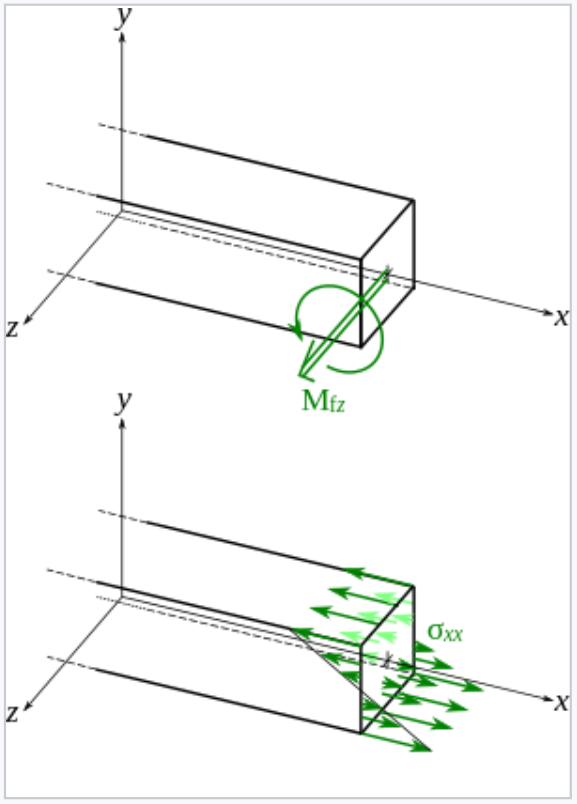
\includegraphics[width=0.45\textwidth]{images/Flexion02.PNG}};
\node () [yshift=-3.5cm]{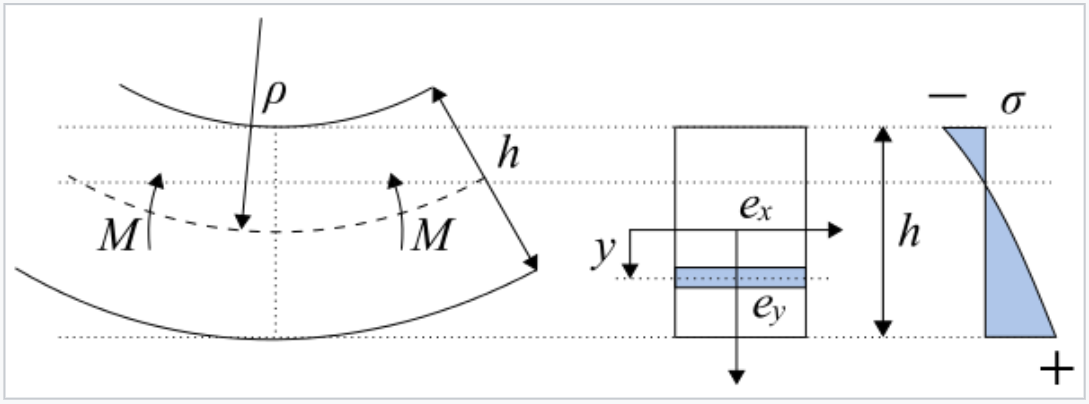
\includegraphics[width=0.50\textwidth]{images/Flexion03.PNG}};

\node () [xshift=-1cm, yshift=-0.5cm] {$ M_{f y} = $ Moment de flexion selon \emph{y}.};
\node () [xshift=-1cm, yshift=-1.0cm] {$ M_{f z} = $ Moment de flexion selon \emph{z}.};
\node () [xshift=-1cm, yshift=-1.5cm] {$ \sigma_{x x} = $ contrainte normale};
\node () [xshift=3.2cm, yshift=-5.8cm] {Rappel : la contrainte normale ($ \sigma $) due à la flexion s'annule à la hauteur du centre de gravité.};

\end{tikzpicture} \end{center}

La valeur de $ \sigma_{x x} $ est donnée par :
\[ \sigma_{x x} = - \frac{M_z}{I_z} y + \frac{M_y}{I_y} z \]
Il faut faire attention aux signes en fonction de comment est placé le repère, la valeur du moment, etc.





\subsection{Inerties Flexionnelles}





%% Tableau d'inerties flexionnelles
\begin{center} \begin{tabular}{cccc}

\begin{tikzpicture}
\node () [rectangle, draw=black, minimum width=1.5cm, minimum height=1.5cm, fill=black!30] {};
\draw [->] (-1.05cm,0cm) -- (1.35cm,0cm) node[anchor=south]{x};
\draw [->] (0cm,-1.05cm) -- (0cm,1.35cm) node[anchor=west] {y};

\draw [<->] (-0.75cm,-1.15cm) -- (0.75cm,-1.15cm);
\node () [yshift=-1.35cm] {a};
\draw [<->] (-1.15cm,-0.75cm) -- (-1.15cm,0.75cm);
\node () [xshift=-1.35cm] {a};
\node () [yshift=-1.95cm] {$\displaystyle I_x = I_y = \frac{a^4}{12} $};
\end{tikzpicture}

&

\begin{tikzpicture}
\node () [rectangle, draw=black, minimum width=1.85cm, minimum height=1.20cm, fill=black!30] {};
\draw [->] (-1.05cm,0cm) -- (1.35cm,0cm) node[anchor=south]{x};
\draw [->] (0cm,-1.05cm) -- (0cm,1.35cm) node[anchor=west] {y};

\draw [<->] (-0.925cm,-1.15cm) -- (0.925cm,-1.15cm);
\node () [yshift=-1.35cm] {b};
\draw [<->] (-1.15cm,-0.60cm) -- (-1.15cm,0.60cm);
\node () [xshift=-1.35cm] {a};
\node () [yshift=-1.95cm] {$\displaystyle I_x = \frac{b a^3}{12} \quad I_y = \frac{a b^3}{12} $};
\end{tikzpicture}

&

\begin{tikzpicture}
\node () [circle, draw=black, minimum width=1.5cm, fill=black!30] {};
\draw [->] (-1.05cm,0cm) -- (1.35cm,0cm) node[anchor=south]{x};
\draw [->] (0cm,-1.05cm) -- (0cm,1.35cm) node[anchor=west] {y};

\draw [<->] (-0.75cm,-1.15cm) -- (0.75cm,-1.15cm);
\node () [yshift=-1.35cm] {d};
\node () [yshift=-1.95cm] {$\displaystyle I_x = I_y = \frac{\pi d^4}{64} $};
\end{tikzpicture}

&

\begin{tikzpicture}
\node () [circle, draw=black, minimum width=1.5cm, fill=black!30] {};
\node () [circle, draw=black, minimum width=1.0cm, fill=white] {};
\draw [->] (-1.05cm,0cm) -- (1.35cm,0cm) node[anchor=south]{x};
\draw [->] (0cm,-1.05cm) -- (0cm,1.35cm) node[anchor=west] {y};

\draw [<->] (-0.75cm,-1.15cm) -- (0.75cm,-1.15cm);
\node () [yshift=-1.35cm] {$ d_e $};
\draw [<->] (-1.15cm,-0.50cm) -- (-1.15cm,0.50cm);
\node () [xshift=-1.35cm] {$ d_i $};
\node () [yshift=-1.95cm] {$\displaystyle I_x = I_y = \frac{\pi (d_e^4 - d_i^4)}{64} $};
\end{tikzpicture}

\end{tabular} \end{center}










\section{Torsion}





\subsection{Explications}





\begin{center} \begin{tikzpicture}

\node () [] {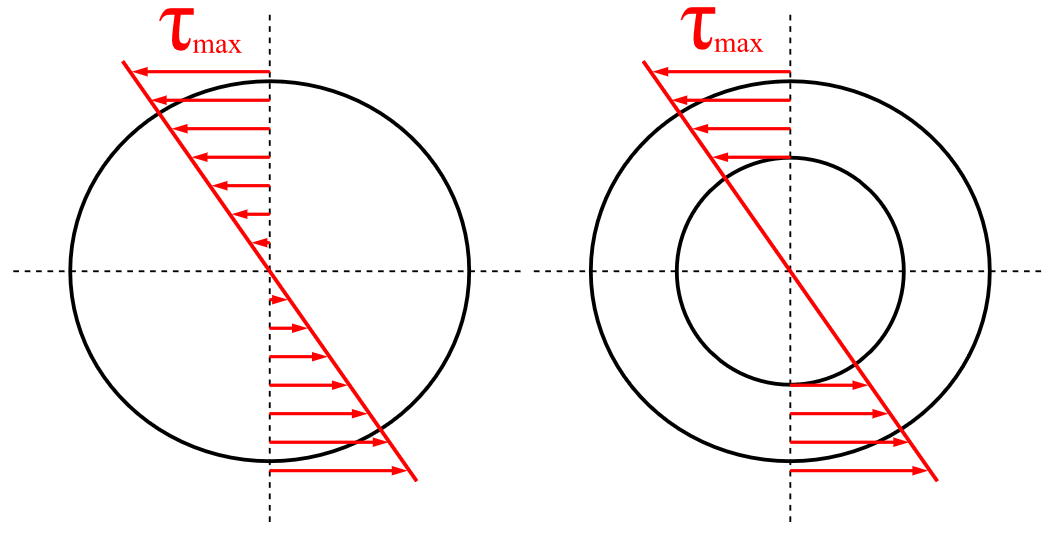
\includegraphics[width=0.4\textwidth]{images/Torsion01.PNG}};
\node () [xshift=7.5cm] {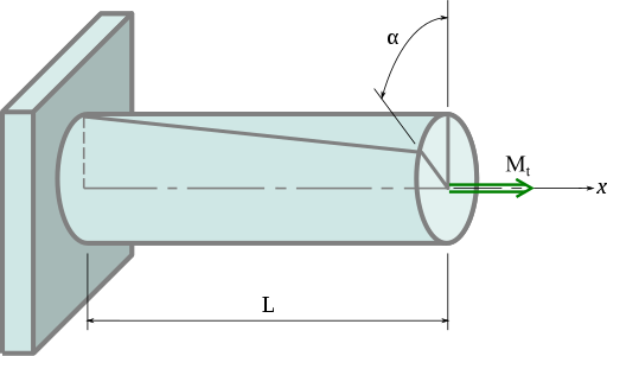
\includegraphics[width=0.5\textwidth]{images/Torsion02.PNG}};

\end{tikzpicture} \end{center}

Le moment de torsion $ M_t $ génère des contraintes de cisaillement $ \tau $ proportionnelles à \emph{r}, la distance par rapport à l'axe de torsion : 
\[ \tau = \frac{M_t}{I_G} r \]
Les déplacements causés par le moment de torsion engendrent aussi un angle de torsion (par unité de longueur) : 
\[ \theta = \frac{\alpha}{L} = \frac{M_t}{G \; I_G} \]
où \emph{G} est le module de cisaillement : $\displaystyle G = \frac{E}{2 (1 + \nu)} $.

Remarque: la torsion est positive lorsqu'elle va dans le sens anti-horaire (sens trigonométrique).





\subsection{Inerties Torsionnelles}





%% Tableau d'inerties flexionnelles
\begin{center} \begin{tabular}{cccc}

\begin{tikzpicture}
\node () [rectangle, draw=black, minimum width=1.5cm, minimum height=1.5cm, fill=black!30] {};
\draw [->] (-1.05cm,0cm) -- (1.35cm,0cm) node[anchor=south]{x};
\draw [->] (0cm,-1.05cm) -- (0cm,1.35cm) node[anchor=west] {y};

\draw [<->] (-0.75cm,-1.15cm) -- (0.75cm,-1.15cm);
\node () [yshift=-1.35cm] {a};
\draw [<->] (-1.15cm,-0.75cm) -- (-1.15cm,0.75cm);
\node () [xshift=-1.35cm] {a};
\node () [yshift=-1.95cm] {$\displaystyle I_g = / $};
\node () [yshift=-2.3cm] {};
\end{tikzpicture}

&

\begin{tikzpicture}
\node () [rectangle, draw=black, minimum width=1.85cm, minimum height=1.20cm, fill=black!30] {};
\draw [->] (-1.05cm,0cm) -- (1.35cm,0cm) node[anchor=south]{x};
\draw [->] (0cm,-1.05cm) -- (0cm,1.35cm) node[anchor=west] {y};

\draw [<->] (-0.925cm,-1.15cm) -- (0.925cm,-1.15cm);
\node () [yshift=-1.35cm] {b};
\draw [<->] (-1.15cm,-0.60cm) -- (-1.15cm,0.60cm);
\node () [xshift=-1.35cm] {a};
\node () [yshift=-1.95cm] {$\displaystyle I_g = / $};
\node () [yshift=-2.3cm] {};
\end{tikzpicture}

&

\begin{tikzpicture}
\node () [circle, draw=black, minimum width=1.5cm, fill=black!30] {};
\draw [->] (-1.05cm,0cm) -- (1.35cm,0cm) node[anchor=south]{x};
\draw [->] (0cm,-1.05cm) -- (0cm,1.35cm) node[anchor=west] {y};

\draw [<->] (-0.75cm,-1.15cm) -- (0.75cm,-1.15cm);
\node () [yshift=-1.35cm] {d};
\node () [yshift=-1.95cm] {$\displaystyle I_g = \frac{\pi d^4}{32} $};
\end{tikzpicture}

&

\begin{tikzpicture}
\node () [circle, draw=black, minimum width=1.5cm, fill=black!30] {};
\node () [circle, draw=black, minimum width=1.0cm, fill=white] {};
\draw [->] (-1.05cm,0cm) -- (1.35cm,0cm) node[anchor=south]{x};
\draw [->] (0cm,-1.05cm) -- (0cm,1.35cm) node[anchor=west] {y};

\draw [<->] (-0.75cm,-1.15cm) -- (0.75cm,-1.15cm);
\node () [yshift=-1.35cm] {$ d_e $};
\draw [<->] (-1.15cm,-0.50cm) -- (-1.15cm,0.50cm);
\node () [xshift=-1.35cm] {$ d_i $};
\node () [yshift=-1.95cm] {$\displaystyle I_g = \frac{\pi (d_e^4 - d_i^4)}{32} $};
\end{tikzpicture}

\end{tabular} \end{center}

Pour l'anneau, lorsque l'épaisseur est très faible ($ e << d_i $), on utilise la formule de Bredt (voir tableau).





\begin{landscape}

\subsection{Tableau}

\begin{center}
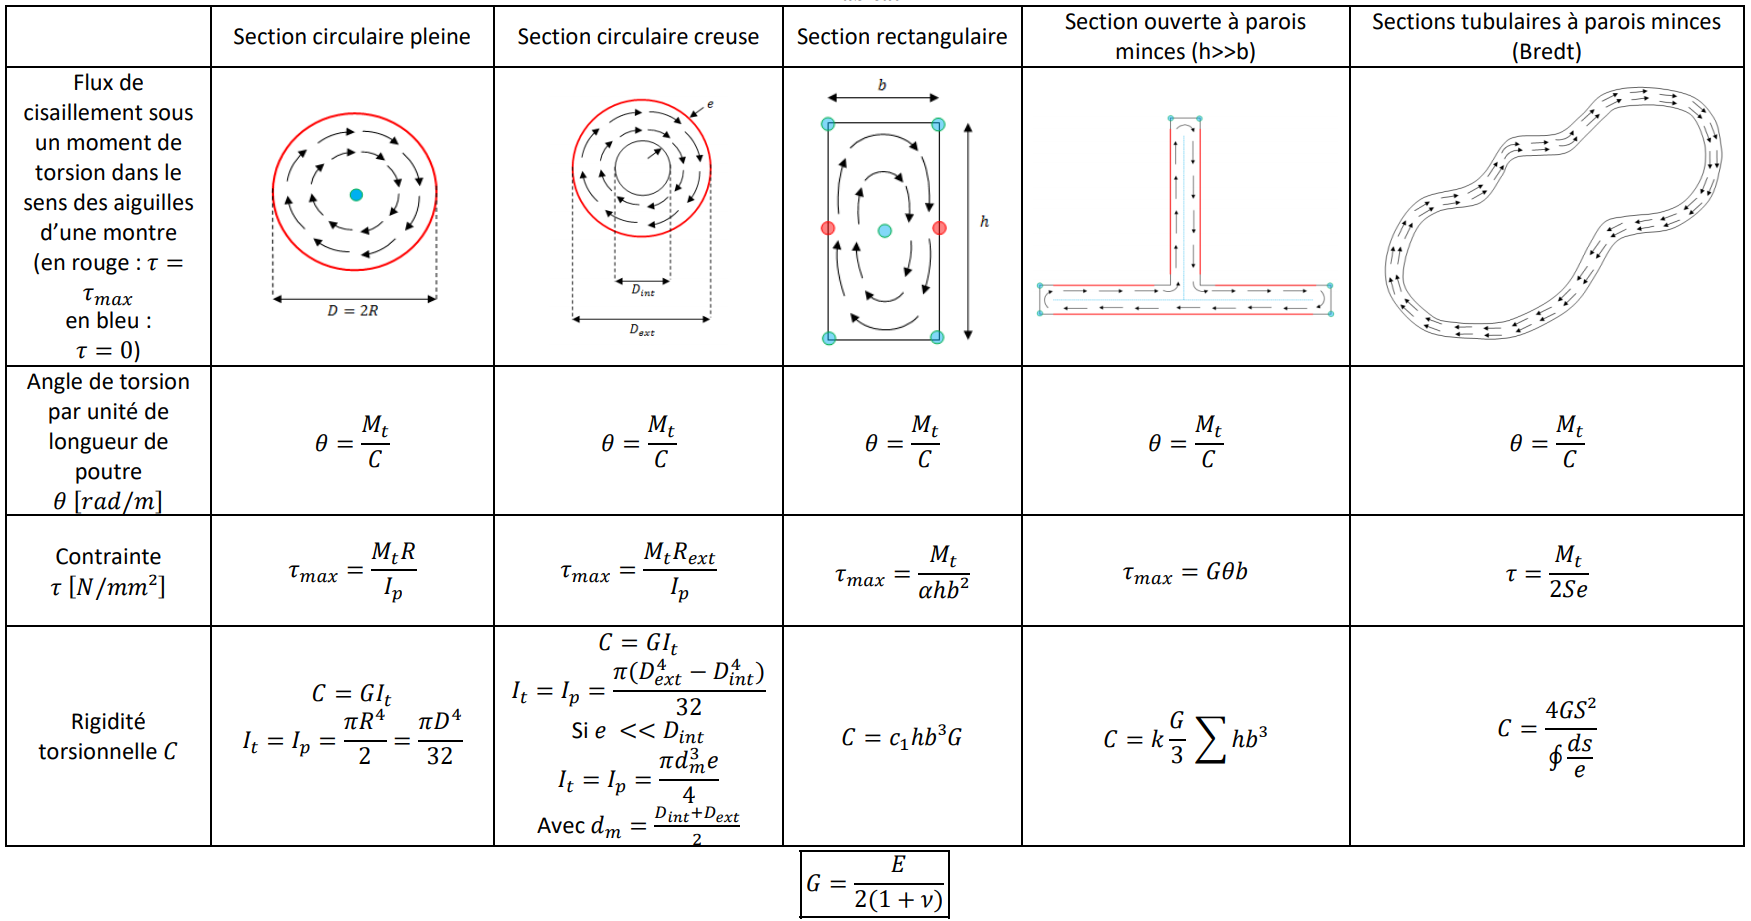
\includegraphics[width=1.55\textwidth]{images/Torsion03.PNG}
\end{center}
\begin{tabular}{c p{14cm}}
Pour une section rectangulaire, on utilise les valeurs de $ \alpha $ et $ c_1 $ suivantes : & On choisit le \emph{k} en fonction de la section de la poutre. \\
\begin{tabular}{|c|cccccc|} \hline
$ n = h / b $ & $ n = 1,00 $ & 1,50 & 2,00 & 3,00 & 4,00 & $ \infty $ \\ \hline
$ \alpha $ & 0,208 & 0,231 & 0,246 & 0,267 & 0,282 & 0,333 \\ \hline
$ c_1 $ & 0,141 & 0,196 & 0,229 & 0,263 & 0,281 & 0,333 \\ \hline
\end{tabular} & 
Pour une poutre en U \& T : k = 1.1, pour les poutres en I (double-T) : k = 1.25. Pour les cornières ($ \Gamma $), k = 1. On a aussi : k = 1 pour les sections tubulaires.
\end{tabular}
\end{landscape}










\section{Cisaillement}





Les efforts tranchants ($ T_x, T_y $) génèrent contraintes tranchantes ($ \tau $) telles que :
\[ \tau = \frac{T \; S_n}{e \; I} \]
où $ S_n $ est le moment statique et \emph{e}, l'épaisseur de la section.

\begin{center} \begin{tikzpicture}

\node () [] {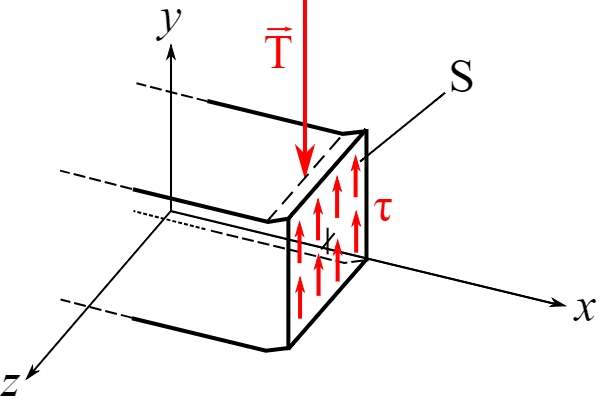
\includegraphics[width=0.5\textwidth]{images/Cisaillement01.PNG}};
\draw[<->] (-0.10cm,-2.25cm) -- (1cm,-1cm);
\node () [xshift=0.5cm, yshift=-1.9cm] {e};
\draw[<->] (-0.40cm,-2cm) -- (-0.40cm,-0.4cm);
\node () [xshift=-0.7cm, yshift=-1cm] {h};

\node () [xshift=6cm, yshift=1cm] {Dans ce cas-ci, on a : $\displaystyle \tau_{y} = \frac{T_y \; S_n}{e \; I_z} $};

\end{tikzpicture} \end{center}





\subsection{Exemples de Distribution des Contraintes de Cisaillement Pur}




\begin{center} \begin{tabular}{cccc}
\begin{tikzpicture}
\node () [circle, draw=black, minimum width=3.5cm, fill=black!10] {};
\node () [circle, draw=black, minimum width=2.5cm, fill=white!100] {};
%% Gauche
\draw[->, thick, red] (95:1.6) arc(95:125:1.6);
\draw[->, thick, red] (130:1.6) arc(130:160:1.6);
\draw[->, thick, red] (165:1.6) arc(165:195:1.6);
\draw[->, thick, red] (200:1.6) arc(200:230:1.6);
\draw[->, thick, red] (235:1.6) arc(235:265:1.6);

\draw[->, thick, red] (95:1.4) arc(95:125:1.4);
\draw[->, thick, red] (130:1.4) arc(130:160:1.4);
\draw[->, thick, red] (165:1.4) arc(165:195:1.4);
\draw[->, thick, red] (200:1.4) arc(200:230:1.4);
\draw[->, thick, red] (235:1.4) arc(235:265:1.4);

\draw[->, thick, red] (85:1.6) arc(85:55:1.6);
\draw[->, thick, red] (50:1.6) arc(50:20:1.6);
\draw[->, thick, red] (15:1.6) arc(15:-15:1.6);
\draw[->, thick, red] (-20:1.6) arc(-20:-50:1.6);
\draw[->, thick, red] (-55:1.6) arc(-55:-85:1.6);

\draw[->, thick, red] (85:1.4) arc(85:55:1.4);
\draw[->, thick, red] (50:1.4) arc(50:20:1.4);
\draw[->, thick, red] (15:1.4) arc(15:-15:1.4);
\draw[->, thick, red] (-20:1.4) arc(-20:-50:1.4);
\draw[->, thick, red] (-55:1.4) arc(-55:-85:1.4);

\draw[-,dashed] (0cm,2cm) -- (0cm,-2cm);
\draw[->, thick] (-0.3,1) -- (-0.3,-1) node[anchor = south east]{\textbf{T}};
\end{tikzpicture}

&

\begin{tikzpicture}
% Fill
\fill[black!10] (-1.75,2) -- (1.75,2) -- (1.75,1.5) -- (-1.75,1.5);
\fill[black!10] (-1.75,-2) -- (1.75,-2) -- (1.75,-1.5) -- (-1.75,-1.5);
\fill[black!10] (-1.75,2) -- (-1.25,2) -- (-1.25,-2) -- (-1.75,-2);

% Horizontal
\draw[-] (-1.75,2) -- (1.75,2);
\draw[-] (-1.75,-2) -- (1.75,-2);
\draw[-] (-1.25,1.5) -- (1.75,1.5);
\draw[-] (-1.25,-1.5) -- (1.75,-1.5);

% Vertical
\draw[-] (-1.75,2) -- (-1.75,-2);
\draw[-] (-1.25,1.5) -- (-1.25,-1.5);
\draw[-] (1.75,2) -- (1.75,1.5);
\draw[-] (1.75,-2) -- (1.75,-1.5);

% Arrows
\draw[->, thick] (1,0) -- (-1,0) node[anchor=south west]{\textbf{T}};
\draw[->, thick, red] (1.7,-1.75) -- (1,-1.75);
\draw[->, thick, red] ($(1.7,-1.75) + (0,3.5)$) -- ($(1,-1.75) + (0,3.5)$);

\draw[->, thick, red] (0.8,-1.75) -- (0.1,-1.75);
\draw[->, thick, red] ($(0.8,-1.75) + (0,3.5)$) -- ($(0.1,-1.75) + (0,3.5)$);

\draw[->, thick, red] (-0.10,-1.75) -- (-0.8,-1.75);
\draw[->, thick, red] ($(-0.10,-1.75) + (0,3.5)$) -- ($(-0.8,-1.75) + (0,3.5)$);

\draw[->, thick, red] (-1.5,-1.75) -- (-1.5,-1);
\draw[->, thick, red] (-1.5,1.75) -- (-1.5,1);

\draw[->, thick, red] (-1.5,-0.75) -- (-1.5,-0.1);
\draw[->, thick, red] (-1.5,0.75) -- (-1.5,0.1);

\end{tikzpicture}

&

\begin{tikzpicture}
% Fill
\fill[black!10] (-1.75,2) -- (1.75,2) -- (1.75,1.5) -- (-1.75,1.5);
\fill[black!10] (-1.75,-2) -- (1.75,-2) -- (1.75,-1.5) -- (-1.75,-1.5);
\fill[black!10] (-1.75,2) -- (-1.25,2) -- (-1.25,-2) -- (-1.75,-2);

% Horizontal
\draw[-] (-1.75,2) -- (1.75,2);
\draw[-] (-1.75,-2) -- (1.75,-2);
\draw[-] (-1.25,1.5) -- (1.75,1.5);
\draw[-] (-1.25,-1.5) -- (1.75,-1.5);

% Vertical
\draw[-] (-1.75,2) -- (-1.75,-2);
\draw[-] (-1.25,1.5) -- (-1.25,-1.5);
\draw[-] (1.75,2) -- (1.75,1.5);
\draw[-] (1.75,-2) -- (1.75,-1.5);

% Arrows
\draw[->, thick] (0,1) -- (0,-1) node[anchor=south east]{\textbf{T}};
\draw[->, thick, red] (1,-1.75) -- (1.7,-1.75);
\draw[->, thick, red] ($(1.7,-1.75) + (0,3.5)$) -- ($(1,-1.75) + (0,3.5)$);

\draw[->, thick, red] (0.1,-1.75) -- (0.8,-1.75);
\draw[->, thick, red] ($(0.8,-1.75) + (0,3.5)$) -- ($(0.1,-1.75) + (0,3.5)$);

\draw[->, thick, red] (-0.8,-1.75) -- (-0.10,-1.75);
\draw[->, thick, red] ($(-0.10,-1.75) + (0,3.5)$) -- ($(-0.8,-1.75) + (0,3.5)$);

\draw[->, thick, red] (-1.5,-1) -- (-1.5,-1.75);
\draw[->, thick, red] (-1.5,1.75) -- (-1.5,1);

\draw[->, thick, red] (-1.5,-0.1) -- (-1.5,-0.75);
\draw[->, thick, red] (-1.5,0.75) -- (-1.5,0.1);
\end{tikzpicture}

&

\begin{tikzpicture}
% Fill
\fill[black!10] (-2,-2) -- (2,-2) -- (2,-1.5) -- (-2,-1.5);
\fill[black!10] (-0.25,2) -- (0.25,2) -- (0.25,-2) -- (-0.25,-2);

% Horizontal
\draw[-] (-2,-2) -- (2,-2);
\draw[-] (-2,-1.5) -- (-0.25,-1.5);
\draw[-] (2,-1.5) -- (0.25,-1.5);
\draw[-] (-0.25,2) -- (0.25,2);
% Vertical
\draw[-] (-2,-2) -- (-2,-1.5);
\draw[-] (2,-2) -- (2,-1.5);
\draw[-] (-0.25,2) -- (-0.25,-1.5);
\draw[-] (0.25,2) -- (0.25,-1.5);
% Arrows
\draw[->, thick] (-2.5,0) -- (-0.5,0) node[anchor=south east]{\textbf{T}};
\draw[->, thick, red] (-1.9,-1.75) -- (-1,-1.75);
\draw[->, thick, red] (-0.8,-1.75) -- (0,-1.75);
\draw[->, thick, red] (0.2,-1.75) -- (1,-1.75);
\draw[->, thick, red] (1.2,-1.75) -- (1.9,-1.75);
\end{tikzpicture}

\end{tabular} \end{center}





\subsection{Calcul de Cisaillement Pur - Exemple}





\begin{center} \begin{tikzpicture}

% Fill
\fill[pattern=north east lines] (4,-2) -- (4,-4) -- (1,-4) -- (1,-2);

% Horizontal
\draw[-] (-4,4) -- (4,4);       % up up
\draw[-] (-4,-4) -- (4,-4);     % down down
\draw[-] (-3,2) -- (4,2);       % up down
\draw[-] (-3,-2) -- (4,-2);     % down up

% Vertical
\draw[-] (-4,4) -- (-4,-4);     % left left
\draw[-] (-3,2) -- (-3,-2);     % left right
\draw[-] (4,4) -- (4,2);        % up right
\draw[-] (4,-4) -- (4,-2);      % down right

% Dashed lines
\draw[-, dashed] (-4.5,3) -- (5.2,3);
\draw[-, dashed] (-4.5,-3) -- (5.2,-3);
\draw[-, dashed] (-3.5,-4.5) -- (-3.5,4.5);
\draw[-, dashed] (1,-1.5) -- (1,-4);
\draw[-, dashed] (4,-1.5) -- (4,-4);
\draw[-, dashed] (-4.5,-1.5) -- (-3,-1.5);
\draw[-, dashed] (4,2) -- (4,4.5);

% Measurements
\draw[<->] (5.2,3) -- node[anchor=west]{h} (5.2,-3);
\draw[<->] (3,4) -- node[anchor=north west]{e} (3,2);
\draw[<->] (-4,1.5) -- node[anchor=south east]{a} (-3,1.5);
\draw[<->] (1,-1.4) -- node[anchor=south]{u} (4,-1.4);
\draw[<->] (-4.3,-1.5) -- node[anchor=east]{y} (-4.3,0);
\draw[<->] (-3.5,4.6) -- node[anchor=south]{b} (4,4.6);

% Arrows
\draw[->, very thick] (-1,1.5) -- (-1,-1.5) node[anchor=south east]{\textbf{T}};
\draw[->, thick] (0,4.5) -- (0,-5) node[anchor=south east]{y};
\draw[->, thick] (-4.5,0) -- node[anchor=south, xshift=0.2cm]{C.G.} (5,0) node[anchor=north east]{x};

% Letters
\node () [xshift=4cm, yshift=-3cm] {$ \bullet $};
\node () [xshift=4cm, yshift=-3cm, anchor=north west] {A};
\node () [xshift=1cm, yshift=-3cm] {$ \bullet $};
\node () [xshift=1cm, yshift=-3cm, anchor=north east] {B};
\node () [xshift=-3.5cm, yshift=-1.5cm] {$ \bullet $};
\node () [xshift=-3.5cm, yshift=-1.5cm, anchor=north west] {C};

% Math
\node () [xshift=8.5cm, yshift=3.5cm] {\fbox{$\displaystyle \tau = \frac{T \; S_n}{e \; I} $}};
\node () [xshift=8.5cm, yshift=2.5cm] {$\displaystyle \tau_A = 0 $};
\node () [xshift=8.5cm, yshift=1cm] 
{$ \begin{aligned} \displaystyle \tau_B &= \frac{T}{e \; I} S_n = \frac{T}{e \; I} \frac{u \; e \; h}{2} \\
&= \frac{T \; u \; h}{2 I} \end{aligned} $};
\node () [xshift=6.5cm, yshift=-0.4cm, text width=6cm, anchor=north west] {avec $ S_{n, B} $ le moment statique de la section hachurée};
\node () [xshift=6.5cm, yshift=-1.5cm, text width=5cm, anchor=north west] {$ I = I_x $ pour tous les calculs (moment de flexion)};

\end{tikzpicture} \end{center}




Pour calculer $ \tau_C $, il faut décomposer $ S_{n, C} $ en deux parties : 




\begin{center} \begin{tikzpicture}

% Fill
\fill[pattern=north east lines] (4,-2) -- (4,-4) -- (-3.5,-4) -- (-3.5,-2);
\fill[pattern=north west lines] (-4,-1.5) -- (-3,-1.5) -- (-3,-3) -- (-4,-3);

% Horizontal
\draw[-] (-4,-4) -- (4,-4);     % down down
\draw[-] (-3,-2) -- (4,-2);     % down up

% Vertical
\draw[-] (-4,2) -- (-4,-4);     % left left
\draw[-] (-3,2) -- (-3,-2);     % left right
\draw[-] (4,-4) -- (4,-2);      % down right

% Dashed lines
\draw[-, dashed] (-4.5,-3) -- (5.2,-3);
\draw[-, dashed] (-3.5,-4.5) -- (-3.5,2.2);
\draw[-, dashed] (-4.5,-1.5) -- (-3,-1.5);
\draw[-, dashed] (4,-2) -- (4,-4.5);

% Measurements
\draw[<->] (5.2,0) -- node[anchor=west]{h} (5.2,-3);
\draw[<->] (-4,1.5) -- node[anchor=south east]{a} (-3,1.5);
\draw[<->] (-4.3,-1.5) -- node[anchor=east]{y} (-4.3,0);
\draw[<->] (-3.5,-4.6) -- node[anchor=south]{b} (4,-4.6);
\draw[<->] (-4.6,-4) -- node[anchor=north east]{e} (-4.6,-2);

% Arrows
\draw[->, thick] (-5,0) -- node[anchor=south, xshift=0.2cm]{C.G.} (5,0) node[anchor=north east]{x};

\end{tikzpicture} \end{center}

On a donc : 
\[ S_{n, C} = \underbrace{\frac{e \; b \; h}{2}}_{\text{Bas}} + \underbrace{\bigg( \frac{h}{2} - y \bigg) \; a \; \bigg[ y + \frac{1}{2} \bigg( \frac{h}{2} - y \bigg) \bigg]}_{\text{Gauche}} = \frac{e \; b \; h}{2} + \frac{a \; h^2}{8} \bigg[ 1 - \bigg( \frac{2 y}{h} \bigg)^2 \bigg] \]
\[ \implies \tau_C = \underbrace{\frac{T e b h}{2 a I}}_{\text{Bas}} + \underbrace{\frac{T h^2}{8 I} \bigg[ 1 - \bigg( \frac{2 y}{h} \bigg)^2 \bigg]}_{\text{Gauche}} \]

Remarque : La contrainte de cisaillement pur est donnée par : $\displaystyle \tau = \frac{T S_n}{e I} $. Pour le rectangle du bas, on remplace les valeurs suivantes dans la formule : $\displaystyle S_{n, C} = \frac{e b h}{2} $, $ T = T_y $, $ I = I_x $ (car il y a une flexion autour de l'axe \emph{x}), on remplace aussi : $ e = a $ puisque \emph{a} est l'épaisseur de la section au point \emph{C}.





\subsection{Centre de Torsion}





\textbf{Définition} : Point par lequel doit passer l'effort tranchant pour qu'il n'en résulte pas un moment de torsion.

\begin{center} \begin{tikzpicture}

% Horizontal
\draw[-] (-4,4) -- (4,4);       % up up
\draw[-] (-4,-4) -- (4,-4);     % down down
\draw[-] (-3,2) -- (4,2);       % up down
\draw[-] (-3,-2) -- (4,-2);     % down up

% Vertical
\draw[-] (-4,4) -- (-4,-4);     % left left
\draw[-] (-3,2) -- (-3,-2);     % left right
\draw[-] (4,4) -- (4,2);        % up right
\draw[-] (4,-4) -- (4,-2);      % down right

% Dashed lines
\draw[-, dashed] (-4.5,3) -- (5.2,3);
\draw[-, dashed] (-4.5,-3) -- (5.2,-3);
\draw[-, dashed] (-3.5,-4.5) -- (-3.5,4.5);
\draw[-, dashed] (4,2) -- (4,4.5);

% Measurements
\draw[<->] (5.2,3) -- node[anchor=west]{h} (5.2,-3);
\draw[<->] (3,4) -- node[anchor=north west]{e} (3,2);
\draw[<->] (-4,1.5) -- node[anchor=south east]{a} (-3,1.5);
\draw[<->] (-3.5,4.6) -- node[anchor=south]{b} (4,4.6);
\draw[<->] (-6,-1) -- node[anchor=north]{t} (-3.5,-1);
\draw[<->] (-3.5,-1) -- node[anchor=north]{d} (0,-1);

% Arrows
\draw[->, very thick] (-6,0) -- (-6,-3) node[anchor=south east]{\textbf{T}};
\draw[->, thick] (0,4.5) -- (0,-5) node[anchor=south east]{y};
\draw[->, thick] (-6.5,0) -- (5,0) node[anchor=north east]{x};
\draw[->, very thick, red] (-1.5,3) -- node[anchor=south west]{\textcolor{red}{\textbf{H}}} (1.5,3);
\draw[->, very thick, red] (1.5,-3) -- node[anchor=south east]{\textcolor{red}{\textbf{H}}} (-1.5,-3);
\draw[->, very thick, red] (-3.5,-1.5) -- node[anchor=south east]{\textcolor{red}{\textbf{V}}} (-3.5,1.5);
 
 % C.T. & C.G.
\node () [] {$ \bullet $};
\node () [anchor=south west, xshift=0.2cm]{C.G.};
\node () [xshift=-6cm] {$ \bullet $};
\node () [xshift=-6cm, anchor=south] {C.T.};
 
\end{tikzpicture} \end{center}



Si on fait les équilibres, on a : 
\begin{itemize}

\item \textbf{H} : $ H - H = 0 $
\item \textbf{V} : $ T - V = 0 $
\item \textbf{M} : $ H h + V d - T (t + d) \implies H h - V t = 0 $

\end{itemize}

On part donc de l'équation : $ H h - V t = 0 $, pour déterminer : $\displaystyle t = \frac{H h}{V} = \frac{H h}{T} $. La valeur de \emph{H} étant : 
\[ H = \int \tau \; d A = \int_0^b \bigg( \frac{T S_n}{e I} \bigg) \; (e \; d u) = \int_0^b \bigg( \frac{T}{e I} \bigg[ u \; e \frac{h}{2} \bigg] \bigg) \; (e \; d u) = \frac{T \; h \; e}{2 I} \int_0^b u \; d u = \frac{T \; h \; e \; b^2}{4 I} \]
Ce qui fait que : 
\[ t = \frac{H h}{T} = \frac{h^2 e b^2}{4 I} \]


Remarques : 
\begin{itemize}

\item Si la section possède 2 axes de symétrie (axes $ \perp $), alors : C.T. = C.G.
\item Si la section est formée de parois planes et minces qui convergent en un point, alors ce point est le C.T.

\end{itemize}

\begin{center} \begin{tikzpicture}
\draw[-, thick] (0,0) -- (0,2); \draw[-, thick] (0,0) -- (2,0); \node () [] {$ \bullet $}; \node () [anchor=north] {C.T.};
\draw[-, thick] (4,0) -- (8,0); \draw[-, thick] (6,0) -- (6,2); \node () [xshift=6cm] {$ \bullet $}; \node () [xshift=6cm, anchor=north] {C.T.};
\end{tikzpicture} \end{center}





\subsection{Sens de \emph{V}, \emph{H} ET \emph{T}}






\begin{center} \begin{tikzpicture}[x=0.5cm, y=-0.5cm, z=-0.3cm, scale=2] % x = right, y = up, z = goes out

% Fill
\fill[black!10] (-1.75,2) -- (1.75,2) -- (1.75,1.5) -- (-1.75,1.5);
\fill[black!10] (-1.75,-2) -- (1.75,-2) -- (1.75,-1.5) -- (-1.75,-1.5);
\fill[black!10] (-1.75,2) -- (-1.25,2) -- (-1.25,-2) -- (-1.75,-2);

\fill[black!10] (-7.75,2,-6) -- (-4.25,2,-6) -- (-4.25,1.5,-6) -- (-7.75,1.5,-6);
\fill[black!10] (-7.75,-2,-6) -- (-4.25,-2,-6) -- (-4.25,-1.5,-6) -- (-7.75,-1.5,-6);
\fill[black!10] (-7.75,2,-6) -- (-7.25,2,-6) -- (-7.25,-2,-6) -- (-7.75,-2,-6);

% Horizontal
\draw[-] (-1.75,2) -- (1.75,2);
\draw[-] (-1.75,-2) -- (1.75,-2);
\draw[-] (-1.25,1.5) -- (1.75,1.5);
\draw[-] (-1.25,-1.5) -- (1.75,-1.5);

% Vertical
\draw[-] (-1.75,2) -- (-1.75,-2);
\draw[-] (-1.25,1.5) -- (-1.25,-1.5);
\draw[-] (1.75,2) -- (1.75,1.5);
\draw[-] (1.75,-2) -- (1.75,-1.5);

% Depth
\draw[-] (-1.75,2,0) -- (-7.75,2,-6);
\draw[-] (-1.75,-2,0) -- (-7.75,-2,-6);
\draw[-] (1.75,-2,0) -- (-4.25,-2,-6);
\draw[-, dashed] (1.75,-1.5,0) -- (-4.25,-1.5,-6);
\draw[-, dashed] (1.75,2,0) -- (-4.25,2,-6);
\draw[-] (1.75,1.5,0) -- (-3.25,1.5,-5); \draw[-, dashed] (-3.25,1.5,-5) -- (-4.25,1.5,-6);

% Horizontal - depth
\draw[-] (-7.75,2,-6) -- (-4.25,2,-6);
\draw[-] (-7.75,-2,-6) -- (-4.25,-2,-6);
\draw[-, dashed] (-7.25,1.5,-6) -- (-4.25,1.5,-6);
\draw[-, dashed] (-7.25,-1.5,-6) -- (-4.25,-1.5,-6);

% Vertical - depth
\draw[-] (-7.75,2,-6) -- (-7.75,-2,-6);
\draw[-, dashed] (-7.25,1.5,-6) -- (-7.25,-1.5,-6);
\draw[-, dashed] (-4.25,2,-6) -- (-4.25,1.5,-6);
\draw[-, dashed] (-4.25,-2,-6) -- (-4.25,-1.5,-6);

% Arrows
\draw[->, very thick, red] (1,-1.75) -- (-1,-1.75) node[anchor=east]{\textcolor{red}{\textbf{H}}};
\draw[->, very thick, red] (-1,1.75) -- (1,1.75) node[anchor=west]{\textcolor{red}{\textbf{H}}};
\draw[->, very thick, red] (-1.5,-1) -- (-1.5,1) node[anchor=north]{\textcolor{red}{\textbf{V}}};
\draw[->, dashed, very thick, red] (-6,1,-6) -- (-6,-1,-6) node[anchor=south]{\textcolor{red}{\textbf{T}}};

% The axes - x = right, y = up, z = goes out
\draw[->, dashdotted] (xyz cs:x=-5) -- (xyz cs:x=5) node[above] {$z$};
\draw[->, dashdotted] (xyz cs:y=-5) -- (xyz cs:y=5) node[right] {$y$};
\draw[->, dashdotted] (xyz cs:z=-6, x=-6) -- (xyz cs:z=5, x=5) node[above] {$x$};
\node () [] {$ \bullet $};
\node at (-6,0,-6){$ \bullet $};

% Text
\node () [xshift=4cm, yshift=4cm, anchor=north west] {On a l'équilibre vertical parce que : $ T - V = 0 $};
\node () [xshift=4cm, yshift=3.5cm, anchor=north west] {Cependant, dans le cours, on dessine parfois $ T // V $};
\node () [xshift=4cm, yshift=3cm, anchor=north west] {On écrit aussi parfois : $\displaystyle \int \tau = T $ au lieu de $ - T $.};
\node () [xshift=4cm, yshift=2cm, anchor=north west] {Bref, c'est pas clair.};

\node () [xshift=4cm, yshift=-1.5cm, anchor=north west, text width=7.5cm] {En fait, le sens n'est pas important car on a les mêmes forces de sens opposés de l'autre coté de la coupe.};

\end{tikzpicture} \end{center}

\begin{center} 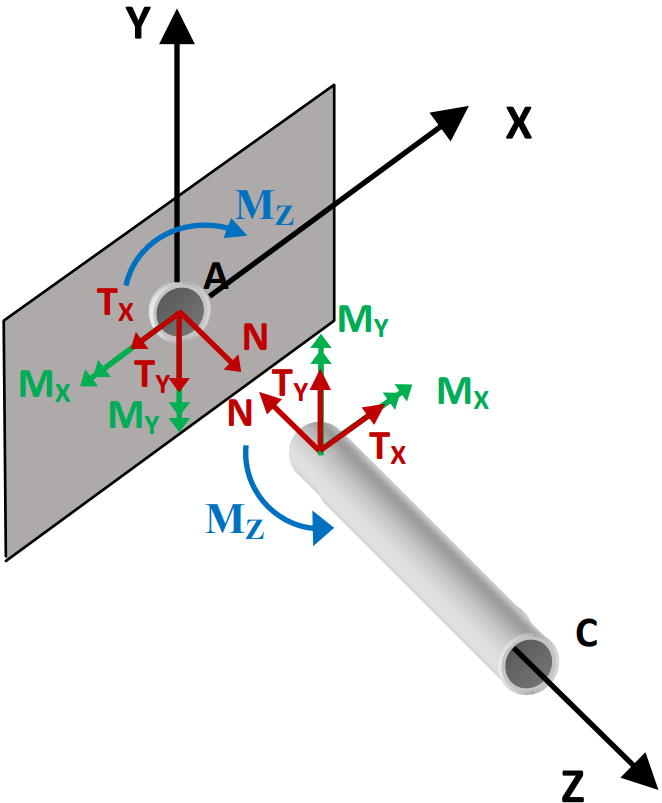
\includegraphics[width=0.5\textwidth]{images/SensMecaMat.PNG} \end{center}





\subsection{Poutre Soumise à son Propre Poids}





\begin{center} 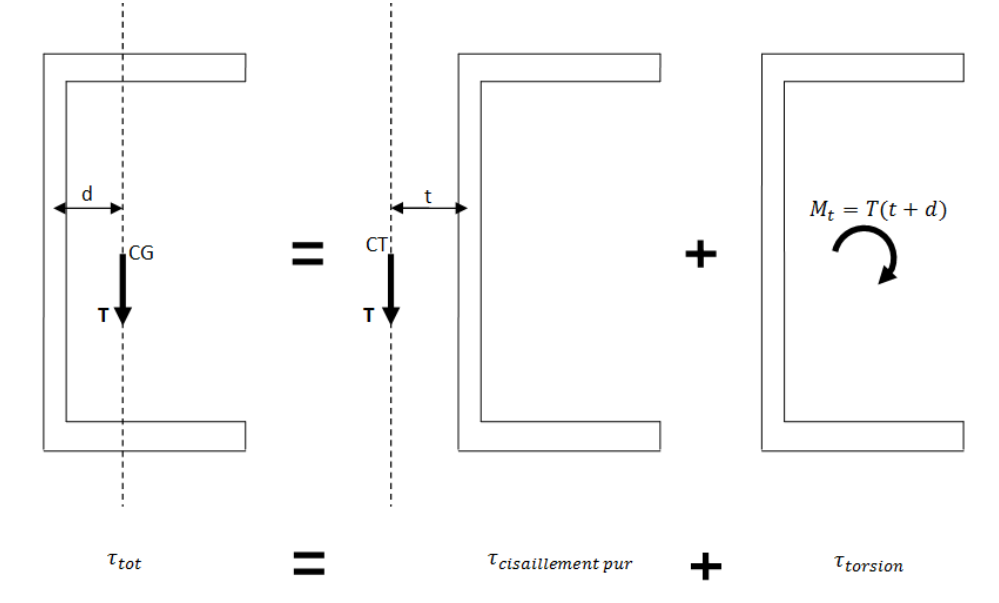
\includegraphics[width=0.85\textwidth]{images/Cisaillement02.PNG} \end{center}










\section{Sollicitations Composées}





\begin{center} \begin{tabular}{|c|c|c|c|c|} \hline &&&& \\
& \textbf{Tension} & \textbf{Flexion} & \textbf{Torsion} & \textbf{Cisaillement} \\ &&&& \\ \hline &&&& \\
\textbf{Sollicitations} & \emph{N} & $ M_z, M_y $ & $ M_T $ & $ T_z, T_y $ \\ &&&& \\ \hline &&&& \\
\textbf{Contraintes} & $\displaystyle \sigma_N = \frac{N}{A} $ & $\displaystyle \sigma_{M_z} = - \frac{M_z}{I_z} \; y, \; \sigma_{M_y} = - \frac{M_y}{I_y} \; z $ & $\displaystyle \tau_{M_t} = \frac{M_t}{I_g} \; r $ & $\displaystyle \tau = \frac{T \; S_n}{e \; I} $ \\ &&&& \\ \hline &&&& \\
\textbf{Déplacements} & $\displaystyle \mathcal{E} = \frac{N}{E \; A} $ & $\displaystyle \mathcal{X} = \frac{M}{E \; I} $ & $\displaystyle \theta = \frac{M_t}{C} $ & $\displaystyle \upgamma_m = \frac{T}{G \; A'} $ \\ &&&& \\ \hline &&&& \\
\textbf{Rigidité} & $ E A $ & $ E I $ & $ C = G I_t $ & $ G A' $ \\ &&&& \\ \hline
\end{tabular} \end{center}





\subsection{Principe de Superposition}





Par ce principe, on a : 
\[ \sigma_{tot} = \sigma_N + \sigma_{M_y} + \sigma_{M_z} \]
\[ \tau_{tot} = \tau_{M_t} + \tau_{T_y} + \tau_{T_z} \]





\subsection{Contraintes de Von Mises \& de Tresca}




\[ \sigma_{\text{V.M.}} = \sqrt{\sigma_{tot}^2 + 3 \times \tau_{tot}^2} \leq Re \]
\[ \sigma_{\text{Tr.}} = \sqrt{\sigma_{tot}^2 + 4 \times \tau_{tot}^2} \leq Re \]










\section{Calcul des Inerties Flexionnelles}





L'inertie flexionnelle selon \emph{x} est donnée par : $\displaystyle I_x = \iint_S y^2 \; d x \; d y $.


%% Tableau d'inerties flexionnelles
\begin{center} \begin{tabular}{cccc}

\begin{tikzpicture}
\node () [rectangle, draw=black, minimum width=1.5cm, minimum height=1.5cm, fill=black!30] {};
\draw [->] (-1.05cm,0cm) -- (1.35cm,0cm) node[anchor=south]{x};
\draw [->] (0cm,-1.05cm) -- (0cm,1.35cm) node[anchor=west] {y};

\draw [<->] (-0.75cm,-1.15cm) -- (0.75cm,-1.15cm);
\node () [yshift=-1.35cm] {a};
\draw [<->] (-1.15cm,-0.75cm) -- (-1.15cm,0.75cm);
\node () [xshift=-1.35cm] {a};
\node () [yshift=-1.95cm] {$\displaystyle I_x = I_y = \frac{a^4}{12} $};
\end{tikzpicture}

&

\begin{tikzpicture}
\node () [rectangle, draw=black, minimum width=1.85cm, minimum height=1.20cm, fill=black!30] {};
\draw [->] (-1.05cm,0cm) -- (1.35cm,0cm) node[anchor=south]{x};
\draw [->] (0cm,-1.05cm) -- (0cm,1.35cm) node[anchor=west] {y};

\draw [<->] (-0.925cm,-1.15cm) -- (0.925cm,-1.15cm);
\node () [yshift=-1.35cm] {b};
\draw [<->] (-1.15cm,-0.60cm) -- (-1.15cm,0.60cm);
\node () [xshift=-1.35cm] {a};
\node () [yshift=-1.95cm] {$\displaystyle I_x = \frac{b a^3}{12} \quad I_y = \frac{a b^3}{12} $};
\end{tikzpicture}

&

\begin{tikzpicture}
\node () [circle, draw=black, minimum width=1.5cm, fill=black!30] {};
\draw [->] (-1.05cm,0cm) -- (1.35cm,0cm) node[anchor=south]{x};
\draw [->] (0cm,-1.05cm) -- (0cm,1.35cm) node[anchor=west] {y};

\draw [<->] (-0.75cm,-1.15cm) -- (0.75cm,-1.15cm);
\node () [yshift=-1.35cm] {d};
\node () [yshift=-1.95cm] {$\displaystyle I_x = I_y = \frac{\pi d^4}{64} $};
\end{tikzpicture}

&

\begin{tikzpicture}
\node () [circle, draw=black, minimum width=1.5cm, fill=black!30] {};
\node () [circle, draw=black, minimum width=1.0cm, fill=white] {};
\draw [->] (-1.05cm,0cm) -- (1.35cm,0cm) node[anchor=south]{x};
\draw [->] (0cm,-1.05cm) -- (0cm,1.35cm) node[anchor=west] {y};

\draw [<->] (-0.75cm,-1.15cm) -- (0.75cm,-1.15cm);
\node () [yshift=-1.35cm] {$ d_e $};
\draw [<->] (-1.15cm,-0.50cm) -- (-1.15cm,0.50cm);
\node () [xshift=-1.35cm] {$ d_i $};
\node () [yshift=-1.95cm] {$\displaystyle I_x = I_y = \frac{\pi (d_e^4 - d_i^4)}{64} $};
\end{tikzpicture}

\end{tabular} \end{center}


Exemple de calcul d'inertie flexionnelle selon \emph{y} : 

\begin{center} \begin{tabular}{cc}
\begin{tikzpicture}

% Fill
\fill[pattern=north east lines] (1.75,2) -- (1.75,1.5) -- (-1.75,1.5) -- (-1.75,2);

% Horizontal
\draw[-] (-1.75,2) -- (1.75,2);
\draw[-] (-1.75,-2) -- (1.75,-2);
\draw[-] (-1.25,1.5) -- (1.75,1.5);
\draw[-] (-1.25,-1.5) -- (1.75,-1.5);

% Vertical
\draw[-] (-1.75,2) -- (-1.75,-2);
\draw[-] (-1.25,1.5) -- (-1.25,-1.5);
\draw[-] (1.75,2) -- (1.75,1.5);
\draw[-] (1.75,-2) -- (1.75,-1.5);

% Axes
\draw[-, dashed] node[anchor=east, xshift=-2.5cm]{\emph{y}} (-2.5,0) -- (2.5,0) node[anchor=west]{\emph{y}};
\draw[-, dashed] node[anchor=north, yshift=-2.5cm]{\emph{x}} (0,-2.5) -- (0,2.5) node[anchor=south]{\emph{x}};

% Measurements
\draw[<->] (-1.75,2.2) -- node[anchor=south west]{b} (1.75,2.2);
\draw[<->] (1.95,1.5) -- node[anchor=west]{e} (1.95,2);
\draw[<->] (1,0) -- node[anchor=west]{$\displaystyle \frac{h}{2} - \frac{e}{2} $} (1,1.75);

\end{tikzpicture}

&

\begin{tikzpicture}

% Fill
\fill[pattern=north east lines] (-1.25,1.5) -- (-1.25,-1.5) -- (-1.75,-1.5) -- (-1.75,1.5);

% Horizontal
\draw[-] (-1.75,2) -- (1.75,2);
\draw[-] (-1.75,-2) -- (1.75,-2);
\draw[-] (-1.25,1.5) -- (1.75,1.5);
\draw[-] (-1.25,-1.5) -- (1.75,-1.5);

% Vertical
\draw[-] (-1.75,2) -- (-1.75,-2);
\draw[-] (-1.25,1.5) -- (-1.25,-1.5);
\draw[-] (1.75,2) -- (1.75,1.5);
\draw[-] (1.75,-2) -- (1.75,-1.5);

% Axes
\draw[-, dashed] node[anchor=east, xshift=-2.5cm]{\emph{y}} (-2.5,0) -- (2.5,0) node[anchor=west]{\emph{y}};
\draw[-, dashed] node[anchor=north, yshift=-2.5cm]{\emph{x}} (0,-2.5) -- (0,2.5) node[anchor=south]{\emph{x}};

% Measurements
\draw[<->] (-1.75,-0.5) -- (-1.25,-0.5) node[anchor=west]{a};
\draw[<->] (-1.95,1.5) -- node[anchor=north east]{$\displaystyle h - 2 e $} (-1.95,-1.5);

\end{tikzpicture}
\end{tabular} \end{center}


Inertie propre rectangle du haut : $\displaystyle I_1 = \frac{b \; e^3}{12} $, terme de transport : $\displaystyle t = b \; e \; \bigg( \frac{h}{2} - \frac{e}{2} \bigg)^2 $. Inertie propre du rectangle de gauche : $\displaystyle I_2 = \frac{a \; (h - 2 e)^3}{12} $.

\[ I_y = 2 \; ( I_1 + t ) + I_2 \]

Remarque : On calcule l'inertie propre à.p.d inerties flexionnelles de bases. Le terme de transport étant donné par : 
\[ t = \text{Aire} \times \Big( \text{distance jusqu'à l'axe} \Big)^2 \]










\section{Moment Statique}





\subsection{Moment Statique d'une Section Tubulaire - Mathématiquement}





\begin{center} \begin{tikzpicture}

\node () [circle, draw=black, minimum width=5cm, fill=white] {};
\node () [circle, draw=black, minimum width=4.0cm, fill=white] {};
\draw [-, thick, dashed] node[anchor=south, xshift=-3cm]{y} (-3cm,0cm) -- (3cm,0cm) node[anchor=south]{y};
\draw [-, thick, dashed] node[anchor=west, yshift = -3cm] {x} (0cm,-3cm) -- (0cm,3cm) node[anchor=west] {x};

\draw [->] (0cm,0cm) -- node[anchor=east]{$ r_e $} (60:2.5cm);
\draw [->] (0cm,0cm) -- node[anchor=north]{$ r_i $} (30:2cm);


\coordinate (c2) at (0,0);

\draw[pattern=north east lines]
% radius=5mm, initial=45, final=270
($(c2) + (225:2cm)$) arc (225:270:2cm)
--
% radius=6mm, reversed
($(c2) + (270:2.5cm)$) arc (270:225:2.5cm)
-- cycle;

\node () [xshift=5cm, yshift=1.5cm, anchor=north west] {$\displaystyle \begin{aligned}
S_{n_x} &= \int_A y \; d A \\
&= \iint y \; d x \; d y \\
&= \int_{3\pi/2}^{5\pi/4} \int_{r_i}^{r_e} r \; \sin \theta \; r \; d r \; d \theta
\end{aligned} $};

\end{tikzpicture} \end{center}

\[ S_{n_x} = \int_{3\pi/2}^{5\pi/4} \sin \theta \; \bigg[ \frac{r_e^3}{3} - \frac{r_i^3}{3} \bigg] \; d \theta = - \cos (5\pi/4) \; \bigg[ \frac{r_e^3}{3} - \frac{r_i^3}{3} \bigg] \]





\subsection{Moment Statique d'une Section Tubulaire - Physiquement}





\begin{center} \begin{tikzpicture}

\node () [circle, draw=black, minimum width=5cm, fill=white] {};
\node () [circle, draw=black, minimum width=4.0cm, fill=white] {};
\draw [-, thick, dashed] node[anchor=south, xshift=-3cm]{y} (-3cm,0cm) -- (0cm,0cm);
\draw [-, thick, dashed] (0cm,0cm) -- (0cm,3cm) node[anchor=west] {x};

\draw [->] (0cm,0cm) -- node[anchor=south]{$ r_e $} (30:2.5cm);
\draw [->] (0cm,0cm) -- node[anchor=north]{$ r_i $} (-30:2cm);


\coordinate (c2) at (0,0);

\draw[pattern=north east lines]
($(c2) + (90:2cm)$) arc (90:180:2cm)
--
% radius=6mm, reversed
($(c2) + (180:2.5cm)$) arc (180:90:2.5cm)
-- cycle;


\coordinate (c4) at (7,0);
\coordinate (CG) at (7,1.06);

\draw[pattern=north east lines]
($(c4) + (180:2.5cm)$) arc (180:0:2.5cm)
-- cycle;

\node at (CG){$ \bullet $};
\node at (CG) [anchor=south west] {\textbf{C.G.}};
\draw[<->] (7,-0.3) -- node[anchor=north]{$ r $} (9.5,-0.3);
\draw[<->] (9.8,0) -- node[anchor=west]{$ h $} (9.8,1.06);
\node () [anchor=north west, xshift=5.5cm,yshift=-0.5cm] {$\displaystyle h = \frac{4 \; r}{3 \; \pi} $};

\end{tikzpicture} \end{center}

Le moment statique de la section hachurée ci-dessus à gauche est donné par : 
\[ \begin{aligned}
S_{n_y} &= S_e \; y_e - S_i \; y_i = \frac{\pi r_e^2}{4} \; \frac{4 r_e}{3 \pi} - \frac{\pi r_i^2}{4} \; \frac{4 r_i}{3 \pi} \\
&= \frac{r_e^3}{3} - \frac{r_i^3}{3}
\end{aligned} \]





\subsection{Tube Elliptique}





\begin{center} \begin{tikzpicture}

\coordinate (c4) at (0,0);
\coordinate (CG) at (0,0.785);

\draw[pattern=north east lines] (0,0) ellipse (2.5cm and 1.85cm);
\draw[fill=white, draw=none] (-2.6,0) -- (-2.6,-1.9) -- (2.6,-1.9) -- (2.6,0);
\draw[-] (-2.5,0) -- (2.5,0);

\node at (CG){$ \bullet $};
\node at (CG) [anchor=south west] {\textbf{C.G.}};
\draw[<->] (0,-0.2) -- node[anchor=north]{$ r $} (2.5,-0.2);
\draw[<->] (2.7,0) -- node[anchor=west]{$ c $} (2.7,0.785);
\node () [anchor=west, xshift=4.5cm,yshift=0.5cm] {$\displaystyle c = \frac{4 \; h}{3 \; \pi} $};
\draw[-, dashed] (-2.7,1.85) -- (0,1.85);
\draw[<->] (-2.7,0) -- node[anchor=east]{$ h $} (-2.7,1.85);

\node () [yshift=-1cm] {Surface = $ \pi r h / 2 $};

\end{tikzpicture} \end{center}










\section{Cercle de Mohr}





Le cercle de Mohr est une représentation graphique de l'état de contrainte. Il permet une résolution graphique de la validation à l'état limite ultime, selon le critère de Tresca (cission maximale).





\subsection{Convention de Signes}





\begin{center}
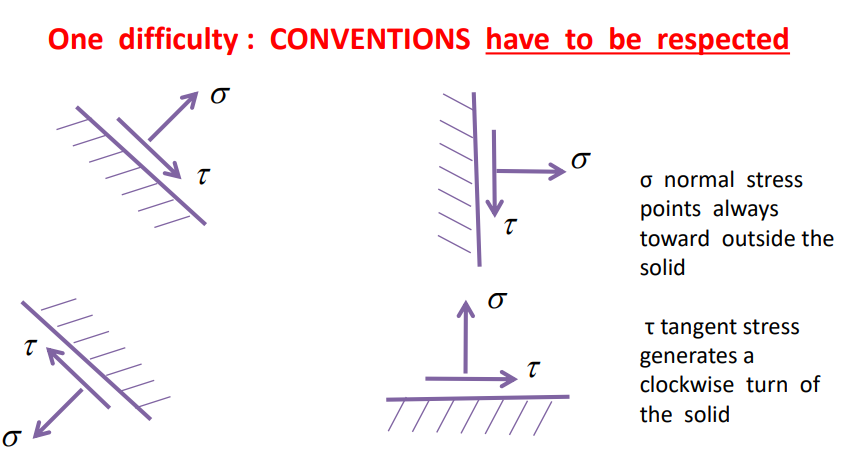
\includegraphics[width=0.49\textwidth]{images/StressConvention.PNG}
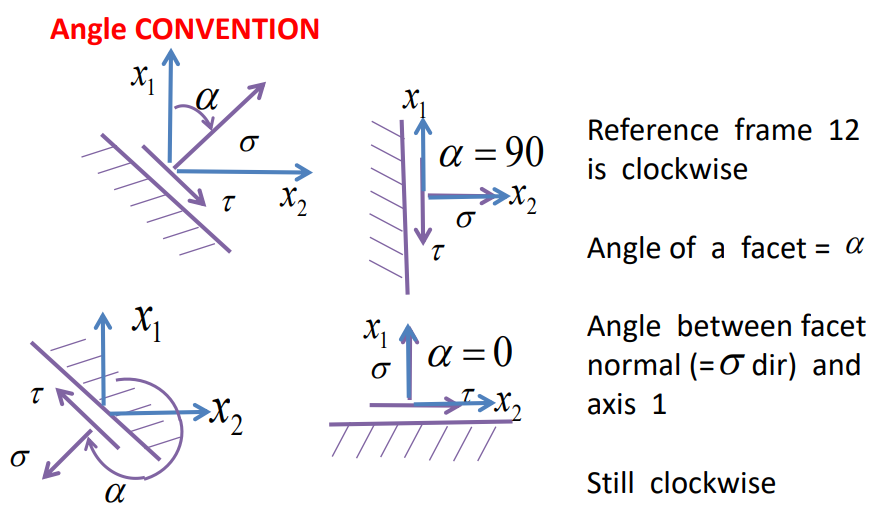
\includegraphics[width=0.49\textwidth]{images/AngleConvention.PNG}
\end{center}





\subsection{Contraintes de Base}





La \textbf{compression} et la \textbf{flexion} engendrent des \textbf{contraintes normales} $ \sigma $. [À gauche] \\
La \textbf{torsion} et le \textbf{cisaillement} engendrent des \textbf{contraintes tangentielles} (de cisaillement) $ \tau $. [À droite]

\begin{center}
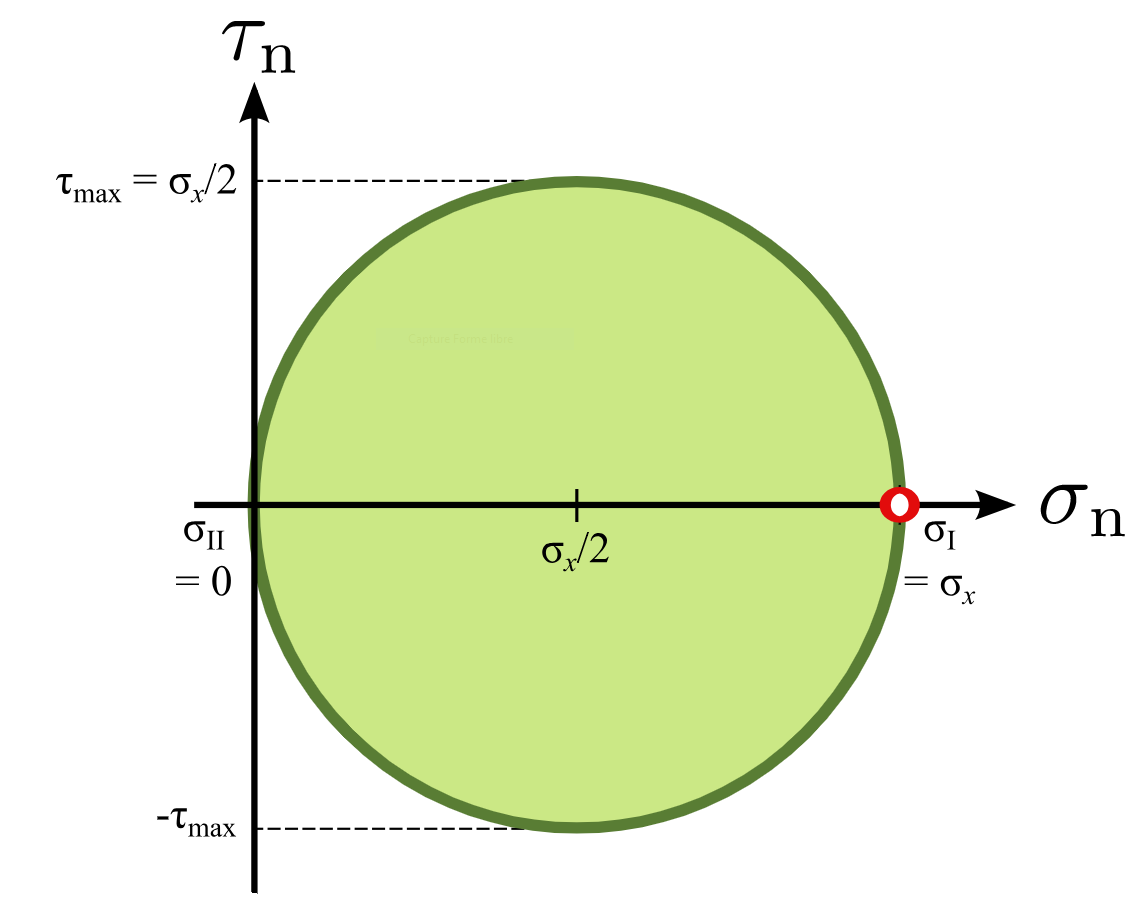
\includegraphics[width=0.54\textwidth]{images/sigmaPurMohr.PNG}
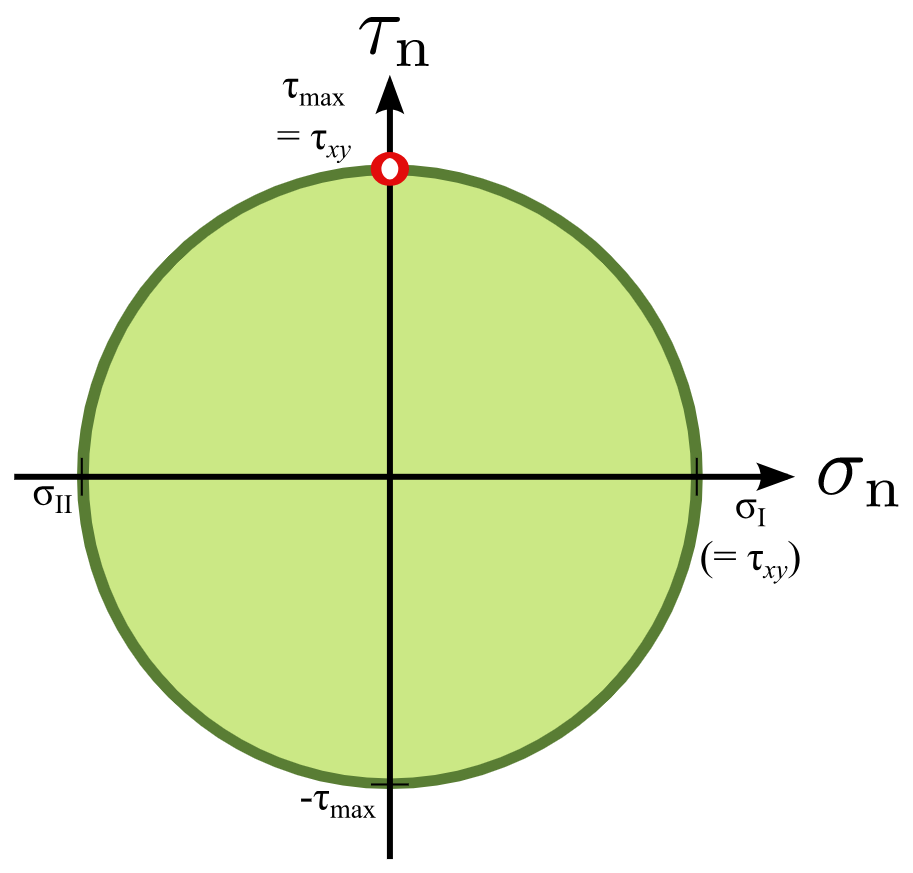
\includegraphics[width=0.44\textwidth]{images/tauPurMohr.PNG}
\end{center}





\subsection{Superposition des Contraintes}





\begin{center}
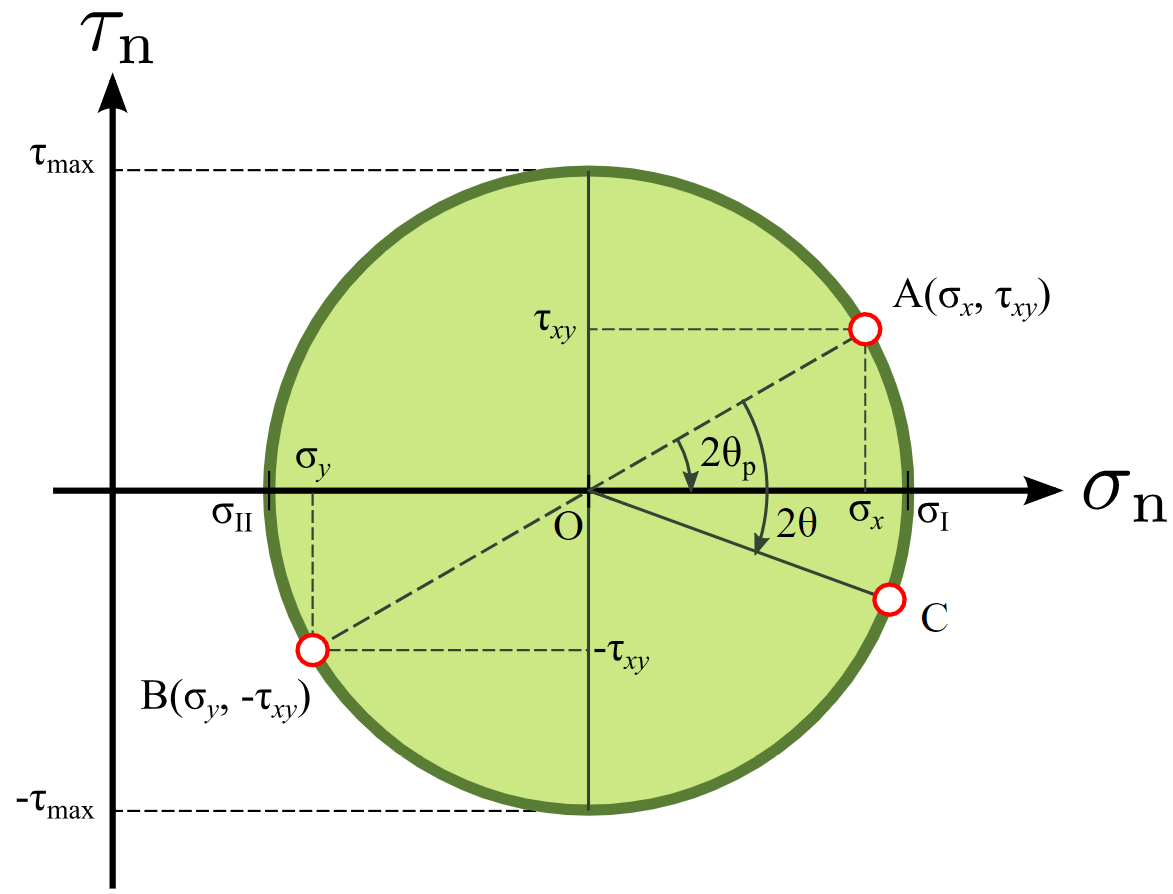
\includegraphics[width=0.6\textwidth]{images/SuperpositionMohr.PNG}
\end{center}





\subsection{Exemple}





\begin{center}
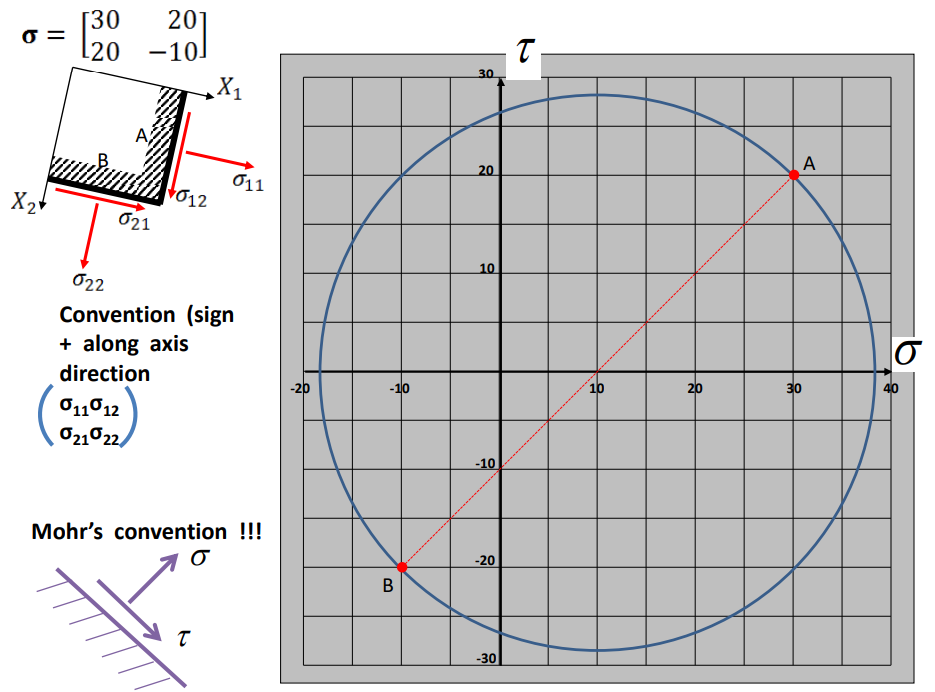
\includegraphics[width=0.75\textwidth]{images/Ex1.PNG}
\end{center}
Ici, on a A = (30, 20) et B = (-10, -20).
\begin{center}
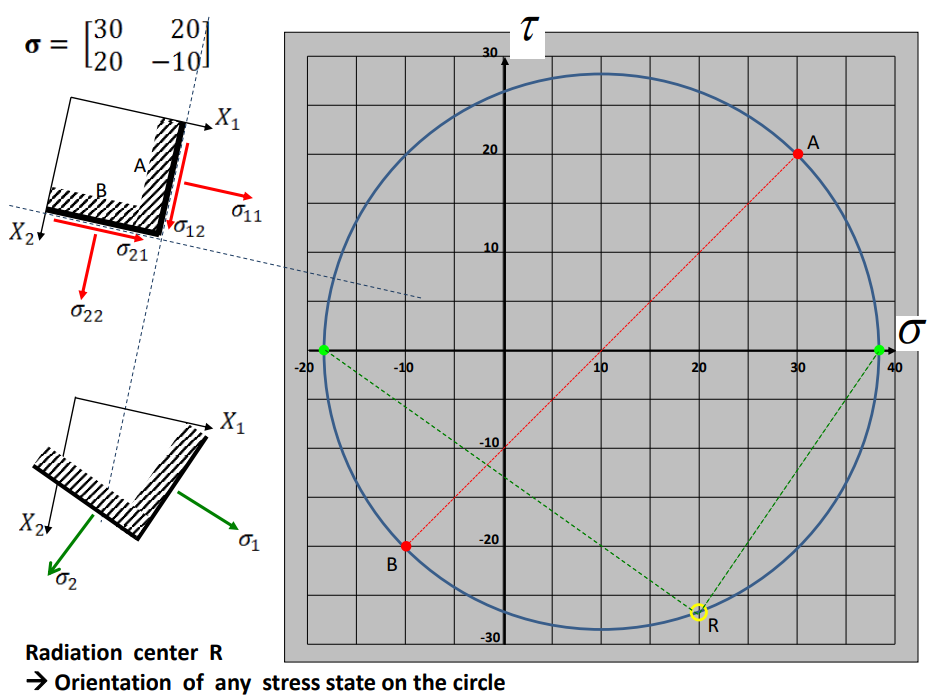
\includegraphics[width=0.75\textwidth]{images/Ex3.PNG}
\end{center}
Ici, on a calculé le centre de rayonnement. En fait, on part de \emph{A} et on trace une droite qui possède la même orientation que la facette \emph{A}. L'intersection entre le cercle de Mohr et la droite que l'on vient de tracer (départ à \emph{A}, orientation $ // $ à \emph{A})
\begin{center}
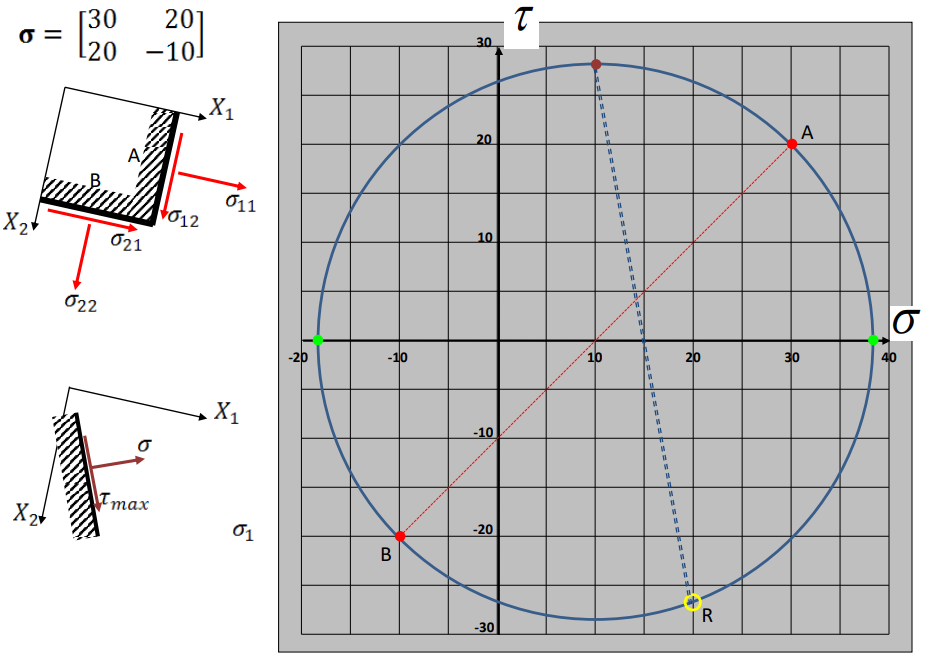
\includegraphics[width=0.75\textwidth]{images/Ex6.PNG} \\
Calcul des contraintes d'une section avec une orientation différente.
\end{center}










\section{Théorie - Anciens Examens}





\subsection{Traction Acier}





\begin{center}
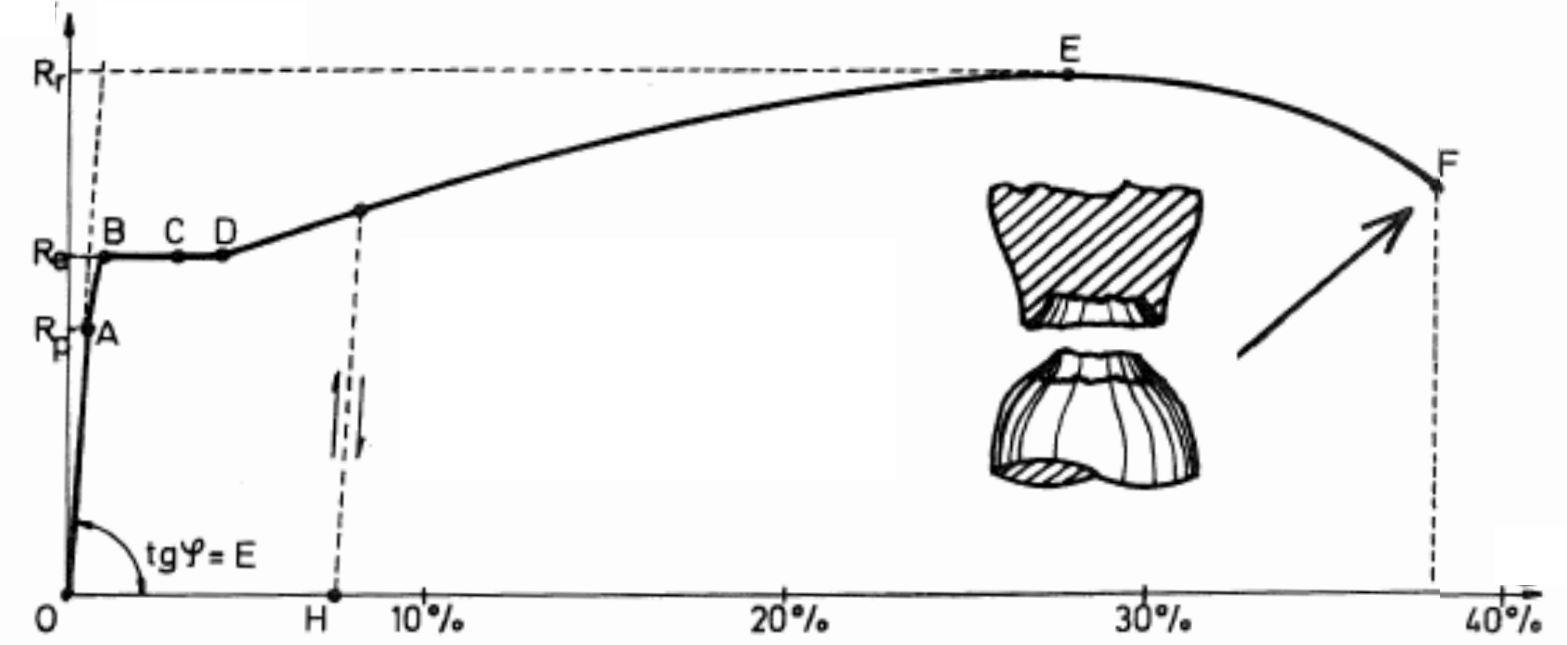
\includegraphics[width=0.75\textwidth]{images/CourbeAcier.PNG}
\end{center}
\begin{itemize}

\item \textbf{Abscisse}: élongation $ \mathcal{E} $ en pourcentage de la longueur de la poutre d'acier (\emph{allongement proportionnel} ou \emph{dilatation}).

\item \textbf{Ordonnée}: contraintes normales $ \sigma $ dans la poutre $ [N/m^2] $.

\item On obtient ce graphique en tirant sur une poutre et en notant la force de traction nécessaire en fonction de l'allongement obtenu. Par exemple, entre B et C, il y a un allongement relativement grand par rapport à la différence de force que l'on a dû exercer sur la poutre. \\
Entre E et F, l'augmentation de l'allongement ne demande pas d'exercer des contraintes plus élevées.

\item \textbf{E} est le module de Young. C'est la "pente" du graphique entre O et A, tel que: 
\[ \sigma = E \; \mathcal{E} \]
Le coefficient \emph{E} est appelé \emph{module d'élasticité longitudinale} ou \emph{module de Young}.

\item $ \textbf{R}_e $ est la limite apparente d'élasticité. À partir du moment où les contraintes normales dans le matériaux ont atteint $ R_e $, le matériaux ne reprendra plus sa forme initiale. Les déformations deviennent permanentes. \\
La contrainte correspondant au point B est appelée \emph{limite d'étirage} ou \emph{limite apparente d'élasticité}, elle est notée $ R_e $.

\item $ \textbf{R}_r $ est la contrainte de rupture. Une fois que l'on a atteint cette valeur, le matériaux rompt. \\
Au point E, la contrainte atteint sa valeur maximum ; cette contrainte est appelée \emph{contrainte de rupture} du matériaux et se note $ R_r $. \\
Ce terme est impropre car la rupture ne se produit pas en E, mais en F (remarque du livre).

\item Le \textbf{coefficient de Poisson} permet de caractériser la contraction de la matière perpendiculairement à la direction de l'effort appliqué.
\[ \mathcal{E}_{lat} = - \nu \; \mathcal{E} = - \nu \; \frac{\sigma}{E} \]

\begin{center}
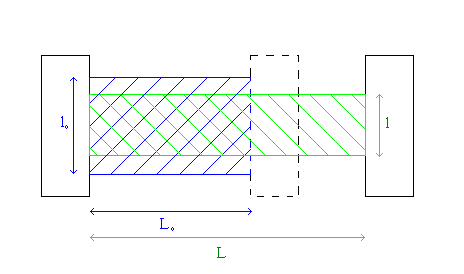
\includegraphics[width=0.3\textwidth]{images/Illustration_pour_coefficient_de_Poisson.png}
\end{center}

\end{itemize}





\subsection{Courbes Caractéristiques}





On demande de dessiner la courbe de comportement caractéristique successivement pour un matériau:
\begin{center} \begin{tabular}{p{6cm}|p{6cm}}
élastique linéaire & élastique non-linéaire \\
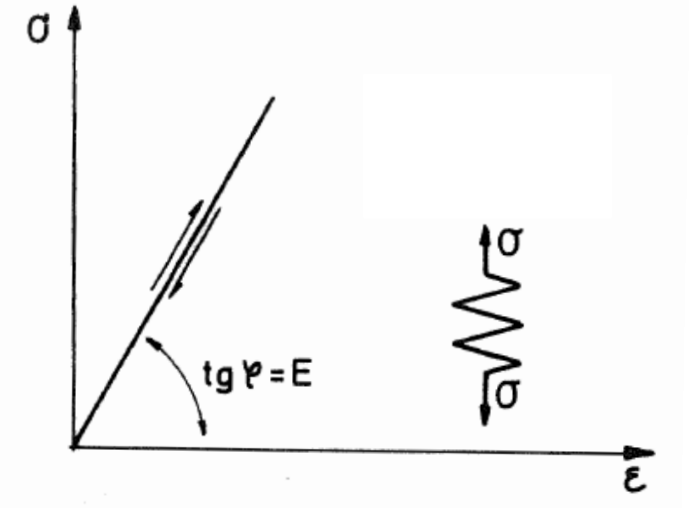
\includegraphics[width=0.3\textwidth]{images/elastiquelineaire.PNG}
&
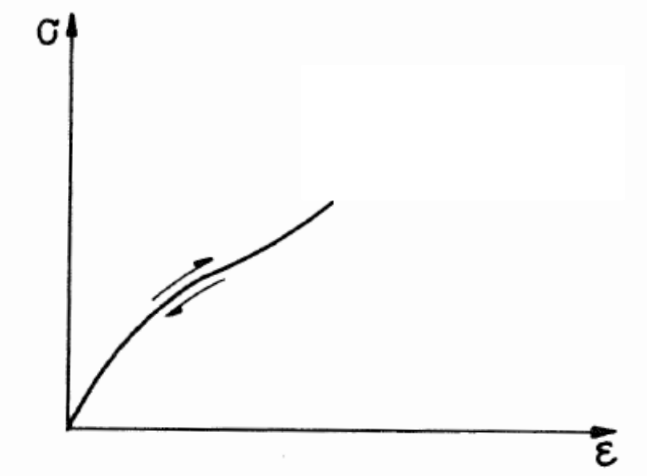
\includegraphics[width=0.3\textwidth]{images/elastiquenonlineaire.PNG}
\\ \hline
élastique linéaire et parfaitement plastique & élastique linéaire, parfaitement plastique mais avec écrouissage \\
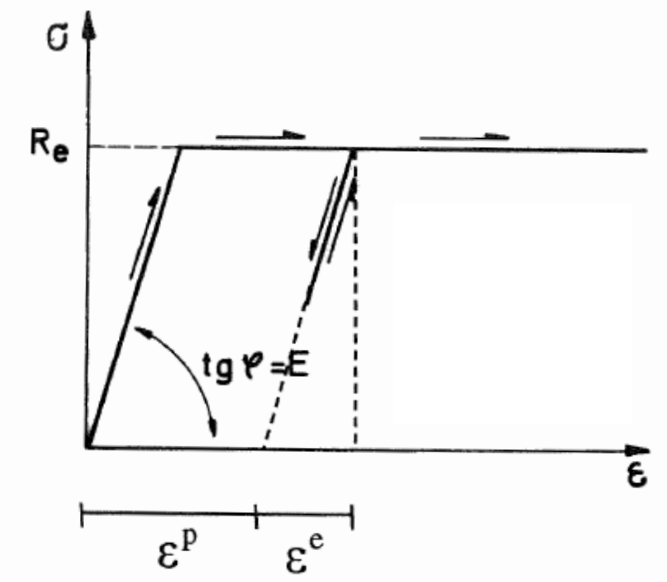
\includegraphics[width=0.3\textwidth]{images/parfaitementplastique.PNG}
&
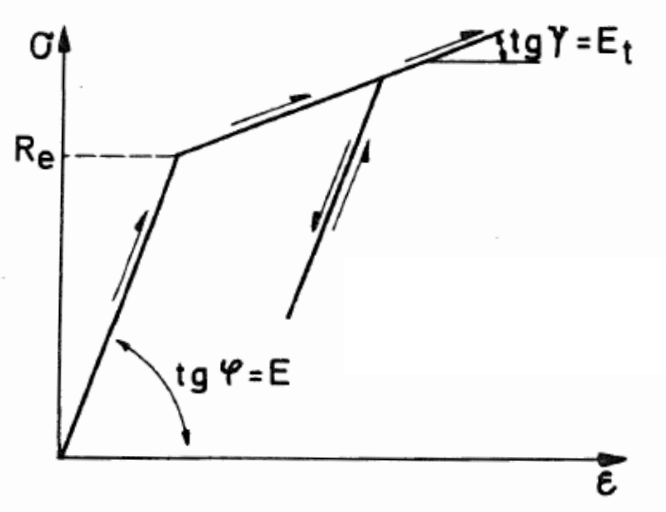
\includegraphics[width=0.3\textwidth]{images/ecrouissage.PNG}
\end{tabular} \end{center}

\textbf{Définition}: le fluage du matériaux est la déformation du matériaux sous des contraintes constantes. (Définition du cours: le \emph{fluage}, qui est la déformation en fonction du temps d'une pièce soumise  à des charges données constantes dans le temps)





\subsection{Résistance Structure}





\begin{siderules}
Dans le cadre du cours de MdM, on s’assure que les charges appliquées à une structure restent
inférieures à celles pour laquelle une limite de résistance serait atteinte en un point de la structure.
Dans la pratique, comment cette « limite de résistance » est-elle exprimée ? En d’autres termes:
\begin{itemize}
    \item définissez physiquement comment est atteinte la limite de résistance d’un matériau ;
    \item fournissez la forme mathématique du(des) critère(s) de vérification de la résistance (dans le cas d’un problème plan) en un point quelconque de la structure, tout en y intégrant les aspects de sécurité.
\end{itemize}
\end{siderules}



\emph{En première approximation}, on peut dire que les matériaux raides se rompent quand la plus grande contrainte principale de traction (positive) $ \sigma_1 $ atteint une valeur déterminée: la contrainte de rupture $ R_r $ déterminée par essai de traction.

\textbf{États limites ultimes d'une structure}: 
\begin{enumerate}[label=(\alph*)]

\item \textcolor{red}{\textbf{Rupture de section critique}}: \\
Si dans une barre tendue, l'effort est tellement grand qu'il crée des contraintes supérieures à la contrainte de rupture du matériau $ R_r $, la barre se rompt.
\[ \text{Critère de Tresca:} \sqrt{\sigma_{tot}^2 + 4 \times \tau_{tot}^2} \leq R_r \]

\item \textcolor{red}{\textbf{Perte de l'équilibre par déplacement anormal d'une partie ou de l'ensemble de la structure}}: \\
Un édifice peut basculer au cours d'un tremblement de terre si le sol qui le porte se dérobe.

\item \textcolor{red}{\textbf{Rupture par fatigue}}: \\
Si une pièce d'acier est soumise à une sollicitation répétée, les contraintes dépassent la limite d'endurance, la rupture se produira nécessairement après un certain nombre de cycles de chargements.
\begin{center}
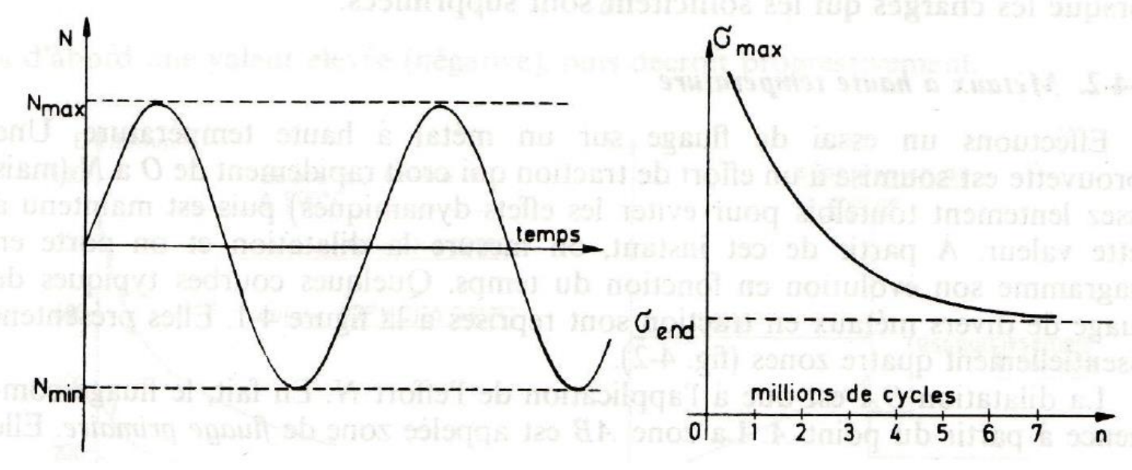
\includegraphics[width=0.75\textwidth]{images/fatigue.PNG}    
\end{center}

\item \textcolor{red}{\textbf{Instabilité}}: \\
Lorsqu'on effectue un essai de compression sur une barre assez élancée, la flèche se dérobe latéralement et périt sous une combinaison de flexion et de compression, plutôt que de compression seul (phénomène de flambement).
\[ \text{Critère:} N \leq P_{cr} = \frac{\pi^2 E I}{L_{fl}^2} \]
\textbf{Vraie charge max ?}
\begin{center}
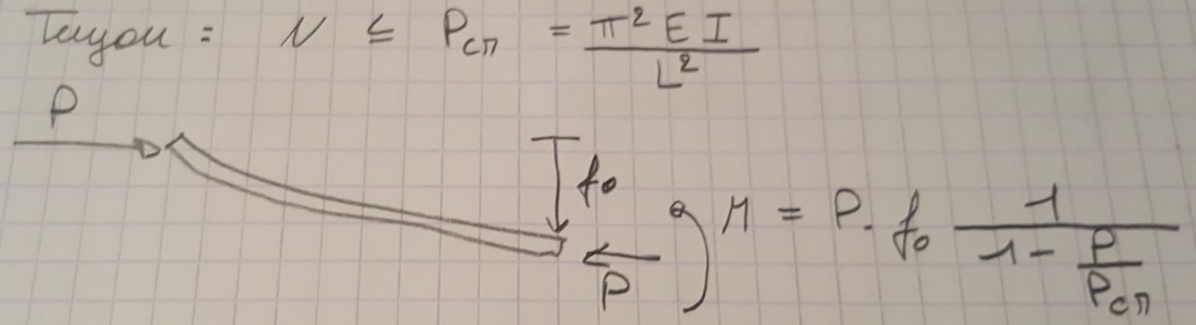
\includegraphics[width=0.75\textwidth]{images/tuyau01.PNG}
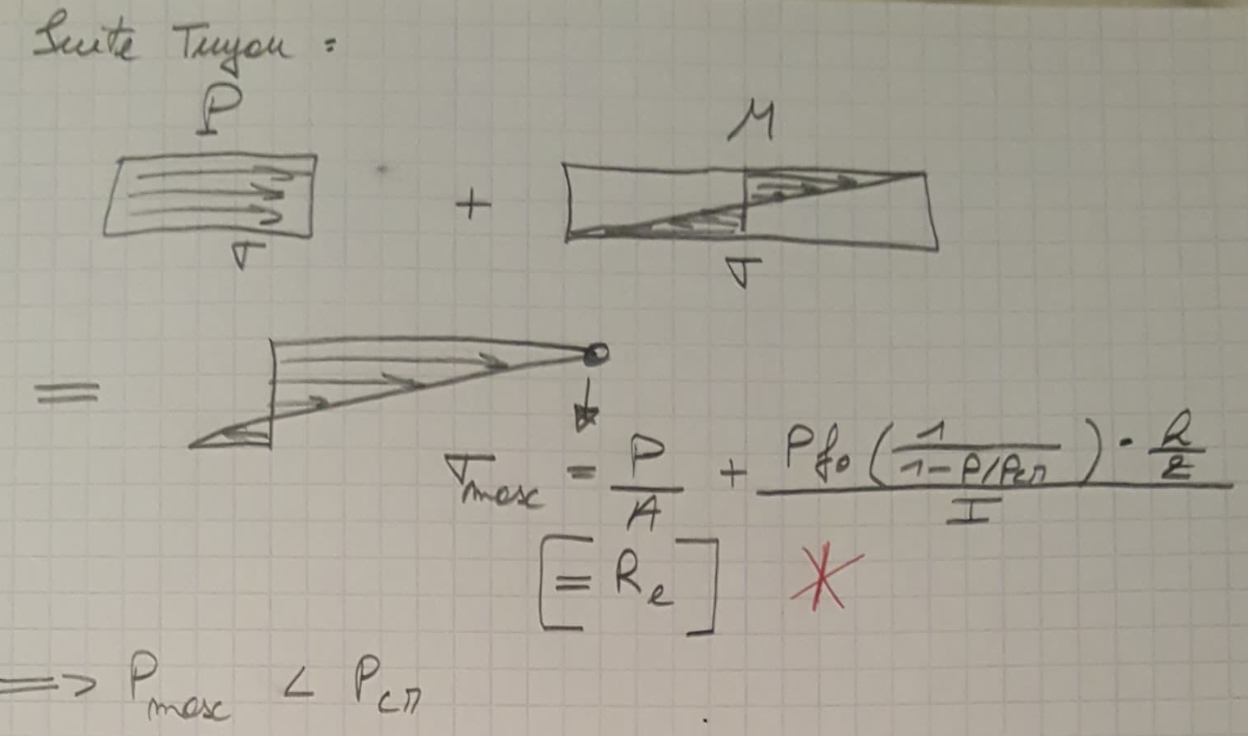
\includegraphics[width=0.75\textwidth]{images/tuyau02.PNG}
\end{center}

\item \textcolor{red}{\textbf{Déformations excessives conduisant à un changement de la géométrie de la structure qui conduit à son effondrement}}: \\
Sur un toi plat, des poches d'eau peuvent se former et engendrent une déformation du toit et surcharger la structure, provoquant son effondrement.

\end{enumerate}



Pour \textbf{vérifier la résistance} en un point quelconque de la structure:
\begin{center}
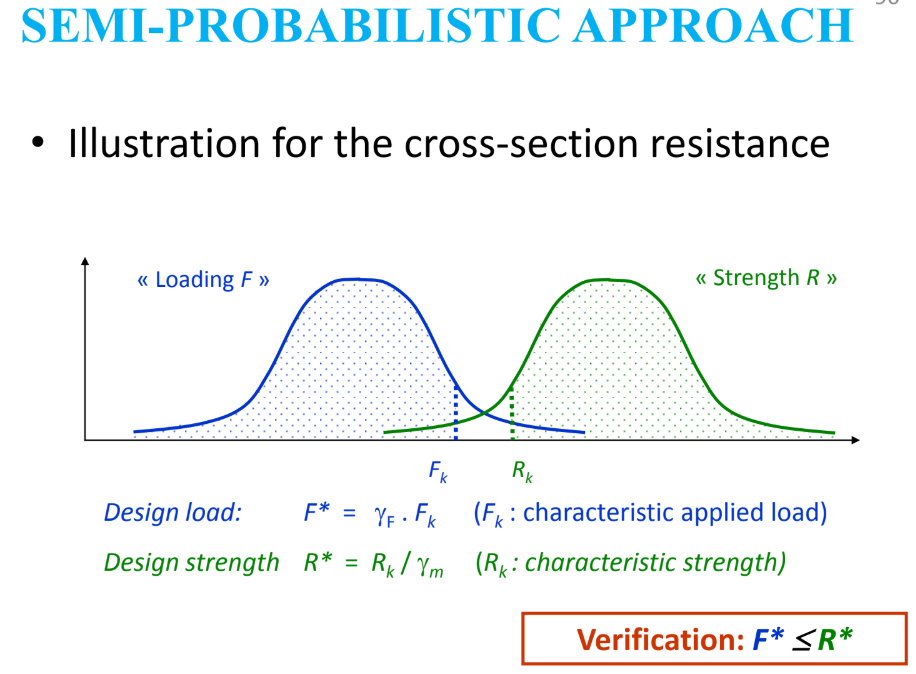
\includegraphics[width=0.75\textwidth]{images/semiprobabilisticResistance.PNG}
\end{center}

Approche semi-probabiliste en 3 étapes:
\begin{enumerate}[label=(\alph*)]

\item Considération des propriétés mécaniques des matériaux et des chargements en tant qu'éléments statistiques.
\[ R_k = R_m - k \; S_r \]
\[ F_k = F_m \pm k S_f \]

\item Les autres facteurs d'incertitude sont couverts en transformant les valeurs caractéristiques en valeurs de calcul.
\[ R^* = R_k / \upgamma_m \]
\[ F^* = F_k / \upgamma_F \]

\item Vérification: sollicitations de calcul $ \leq $ état-limite.
\[ \sigma_c^* \leq R^* \qquad \text{et} \qquad F^* \leq R^* \]
($ \sigma_c^* $ obtenu avec Tresca, c-à-d: $ \sigma_c^* = \sqrt{\sigma^2+4 \tau^2} $)

\end{enumerate}
But du calcul: maintenir la probabilité d'atteindre l'état limite envisagé en deçà d'une certaine valeur préalablement établie pour le type de structure considérée.



\textbf{Coefficient de sécurité}: On mesure l'ensemble des incertitudes affectant la sécurité d'une structure  par un coefficient de sécurité global \emph{s}: 
\[ \sigma_k \leq \frac{R_k}{s} \]





\subsection{Tableau Efforts et Déformations}





\begin{siderules}
\begin{enumerate}[label=(\alph*)]
    \item Dans l’espace, on identifie, en chaque section de poutre le long de son axe, un ensemble de 6 efforts intérieurs : un effort axial N, deux moments de flexion M, deux efforts tranchants V et un moment de torsion MT. Ces quatre grands types d’efforts sont repris dans la première colonne du tableau.
    \item Chacun de ces efforts engendre dans les sections correspondantes des déformations. Quelles sont-elles ?
    \item Le cours de MdM fournit des méthodes de détermination de ces déformations pour chacun des six efforts. Pourriez-vous compléter le tableau avec ces formules ?
    \item Pour chacune de ces formules, pourriez-vous définir les variables qu’elles font intervenir et préciser les conditions éventuelles ou les limites d’utilisation à satisfaire afin de pouvoir les utiliser?
\end{enumerate}
\end{siderules}


\begin{center} \begin{tabular}{|c|c|c|c|c|} \hline &&&& \\
& \textbf{Tension} & \textbf{Flexion} & \textbf{Torsion} & \textbf{Cisaillement} \\ &&&& \\ \hline &&&& \\
\textbf{Sollicitations} & \emph{N} & $ M_z, M_y $ & $ M_T $ & $ T_z, T_y $ \\ &&&& \\ \hline &&&& \\
\textbf{Contraintes} & $\displaystyle \sigma_N = \frac{N}{A} $ & $\displaystyle \sigma_{M_z} = - \frac{M_z}{I_z} \; y, \; \sigma_{M_y} = - \frac{M_y}{I_y} \; z $ & $\displaystyle \tau_{M_t} = \frac{M_t}{I_g} \; r $ & $\displaystyle \tau = \frac{T \; S_n}{e \; I} $ \\ &&&& \\ \hline &&&& \\
\textbf{Déplacements} & $\displaystyle \mathcal{E} = \frac{N}{E \; A} $ & $\displaystyle \mathcal{X} = \frac{M}{E \; I} $ & $\displaystyle \theta = \frac{M_t}{C} $ & $\displaystyle \upgamma_m = \frac{T}{G \; A'} $ \\ &&&& \\ \hline &&&& \\
\textbf{Rigidité} & $ E A $ & $ E I $ & $ C = G I_t $ & $ G A' $ \\ &&&& \\ \hline
\end{tabular} \end{center}


\textbf{Hypothèses traction/compression}: allongement et répartition des contraintes uniformes.

\textbf{Hypothèse flexion}: courbure constante - se déforme en un arc de cercle.

\textbf{Hypothèses torsion}: 
\begin{itemize}
    \item toutes les sections tournent autour de leur centre respectif
    \item toutes les sections restent planes
    \item un rayon quelconque tracé dans une section droite reste rectiligne
    \item l'angle entre 2 rayons ne peut pas varier.
\end{itemize}

\textbf{Hypothèse cisaillement}: on suppose que les sections droites restent planes (même si c'est faux en pratique).





\subsection{Flambement}





\begin{center}
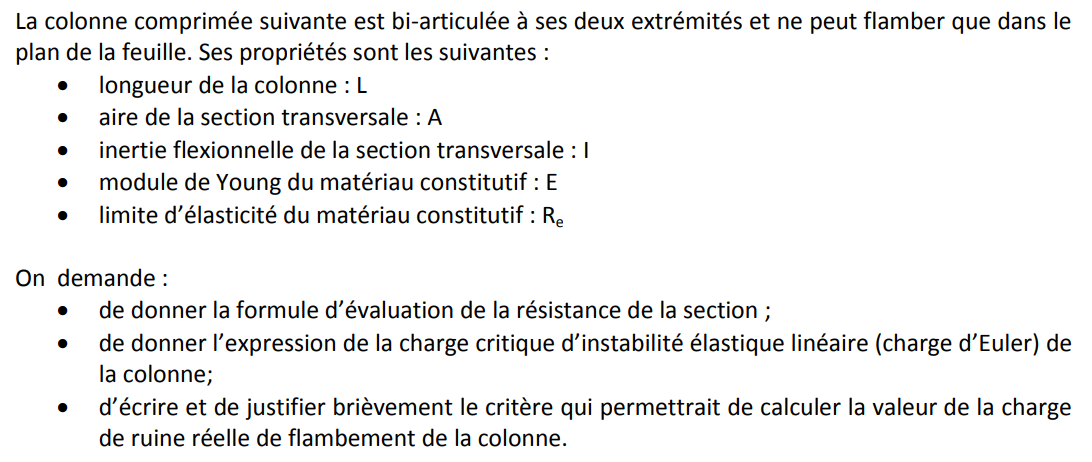
\includegraphics[width=0.85\textwidth]{images/enonceflambement.PNG}
\end{center}
\begin{tikzpicture}

%% texte - Mohr
\node[anchor=north west] at (0,0) 
{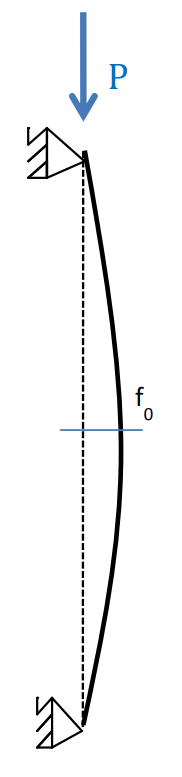
\includegraphics[width=0.175\textwidth]{images/PoutreBiArticulee.PNG}};
\node[anchor=north west, text width=11cm] at (4,-0.5)
{Critère de résistance de la section (cercle de Mohr): 
\[ \sigma_{max} = \frac{P}{A} \qquad \tau_{max} = \frac{1}{2} \frac{P}{A} \]};

%% Dessin Mohr
\draw[->] (4.5,-9) -- (4.5,-3) node[anchor=south]{$ \tau $};
\draw[->] (4,-6) -- (10,-6) node[anchor=west]{$ \sigma $};
\draw[-] (4.5,-6) arc (180:-180:2.5cm);
\draw[-, dashed] (4.5,-3.5) node[anchor=east]{$ \tau_{max} $} -- (7,-3.5);
\node[anchor=north west] at (9.5,-6) {$ \sigma_{max} $};
\node[anchor=north west] at (10,-4) {$\displaystyle \sqrt{\sigma_{max}^2 + 4 \times \tau_{max}^2} \leq R_e $};

%% texte - charge critique d'instabilité
\node[anchor=north west, text width=11cm] at (4,-9.5)
{Charge critique d'instabilité:
\[ P_{cr} = \frac{\pi^2 E I}{L_{fl}^2} \]};

\end{tikzpicture}

\textbf{Vraie charge max ?}
\begin{center}
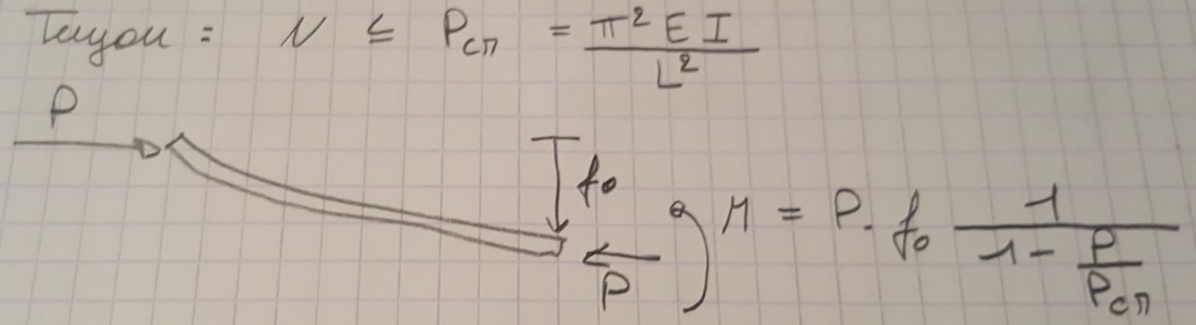
\includegraphics[width=0.75\textwidth]{images/tuyau01.PNG}
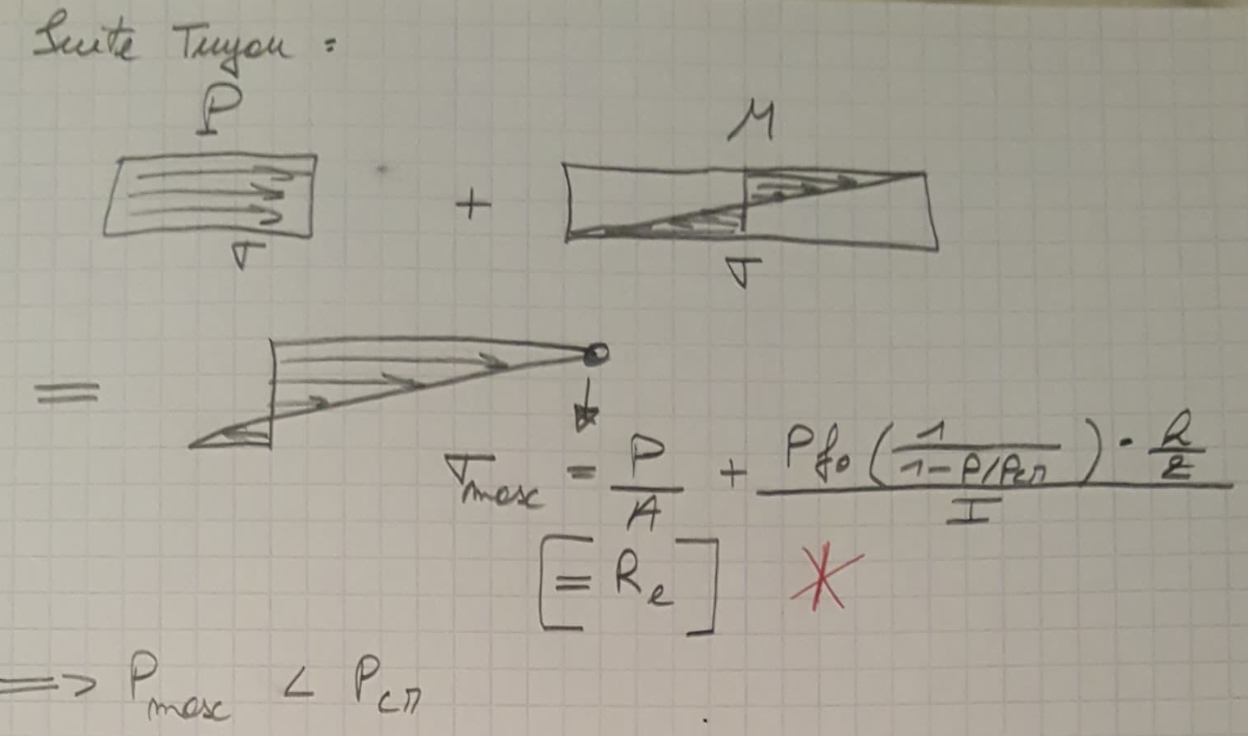
\includegraphics[width=0.75\textwidth]{images/tuyau02.PNG}
\end{center}





\subsection{Noyau Central}





\begin{siderules}
Précisez clairement et précisément ce que l’on entend par le « noyau central » d’une section ! \\
Dérivez son expression mathématique et dessinez-le dans le cas d’une section transversale rectangulaire de largeur b et de hauteur h !
\end{siderules}


La région dans laquelle la force de compression peut être appliquée sans produire aucune contrainte de traction dans la section droite est le noyau central de la section.
\begin{center}
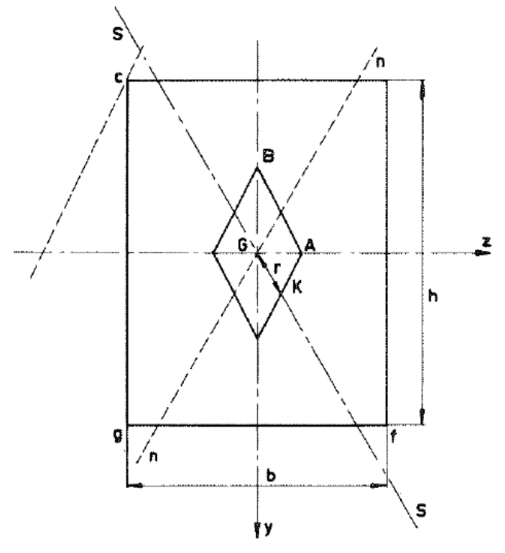
\includegraphics[width=0.5\textwidth]{images/noyaucentral.PNG}
\end{center}
Dans le cas d'une section rectangulaire, lorsque la charge est appliquée au point A (distance b/6 du centre de gravité G), la ligne de contraintes nulles coïncide avec le coté \emph{cg}. \\
De la même manière, lorsque la charge est au point B, à la distance h/6 du centre de gravité G, la ligne de contraintes nulles coïncide avec le coté \emph{gf}. \\
AB est un des cotés du noyau central, les autres cotés se déduisent par symétrie. \textit{Le noyau central est donc un losange dont les diagonales ont des longueurs h/3 et b/3.}


\begin{siderules}
\textbf{Noyau central}: de nombreux matériaux de construction, comme les briques, la pierre ou le béton non armé, ne peuvent supporter en toute sécurité, que des contraintes normales de compression. On doit donc déterminer dans quelle partie de la section doit se trouver le point de passage C de la force extérieure pour que la section soit entièrement comprimée. Cette partie de la section est appelée noyau central.

On doit déterminer où:
\[ \sigma = \frac{N}{S} + \frac{M \; y}{I} \geq 0 \]
Soit,
\[ \frac{M}{N} = GC > - \frac{I}{S \; y} \qquad \text{ si } y > 0 \]
\[ \frac{M}{N} = GC < - \frac{I}{S \; y} \qquad \text{ si } y < 0 \]

Dans le cas d’une section rectangulaire de largeur b et de hauteur h on doit avoir (règle du tiers central):
\[ -h/6 < CG < h/6 \]
\end{siderules}


\begin{center}
\includegraphics[width=0.75\textwidth]{images/noyaucentralg.PNG}
\end{center}





\subsection{Variation des Sections Droites}





\begin{center}
\includegraphics[width=0.85\textwidth]{images/enoncesection.PNG}
\end{center}

\begin{center}
\includegraphics[width=0.75\textwidth]{images/changementSection.PNG}
\end{center}
\[ \sigma_{max} = k \; \sigma_{moyen} \]





\subsection{Matériau ductile/fragile}





\begin{siderules}
Qu’entend-on par matériau fragile et matériau ductile en MdM ? \\
Précisez, à l’aide de mots et d’un diagramme approprié, leurs particularités en matière de comportement mécanique ! \\
Enfin, quelle est l’influence de la nature fragile ou ductile du matériau sur le critère de résistance à mettre en œuvre en MdM?
\end{siderules}

La \textbf{ductilité} désigne la capacité d'un matériau à se déformer plastiquement sans se rompre. La rupture se fait lorsqu'un défaut (fissure ou cavité) devient critique et se propage. La ductilité est donc l'aptitude d'un matériau à résister à cette propagation. S'il y résiste bien, il est dit ductile, \textbf{sinon} il est dit \textbf{fragile}.

\begin{center}
\includegraphics[width=0.75\textwidth]{images/ductilefragile.PNG}
\end{center}





\subsection{Poutre Encastrée-Libre}





\begin{center}
\includegraphics[width=0.85\textwidth]{images/enoncepoutre01.PNG}
\end{center}
\begin{center}
\includegraphics[width=0.85\textwidth]{images/enoncepoutre02.PNG}
\end{center}


\begin{tikzpicture}

% structure
\draw[-] (0,0.25) -- (0,-0.25);
\fill[pattern=north east lines] (0,0.25) -- (-0.35,0.25) -- (-0.35,-0.25) -- (0,-0.25);
\draw[-, thick] (0,0) -- (3,0);

% force
\draw[->, thick] (3.2,0.3) arc (95:-80:0.3); \node[anchor=east] at (4.15,0) {$ M_c $};
\draw[->] (5.1,0) -- (4.1,0) node[anchor=south west]{P};

% diagramme N
\draw[-, thick] (0,-1) node[anchor=east]{\textbf{N}} -- (3,-1);
\draw (0,-1) -- (0,-0.5) -- node[anchor=north]{-P} (3,-0.5) -- (3,-1);

% diagramme T
\draw[-, thick] (0,-2) node[anchor=east]{\textbf{T}} -- node[]{/} node[anchor=south, yshift=0.2cm]{0} (3,-2);

% diagramme M
\draw[-, thick] (0,-3) node[anchor=east]{\textbf{M}} -- (3,-3);
\draw (0,-3) -- (0,-2.5) -- node[anchor=north]{$ - M_c $} (3,-2.5) -- (3,-3);

% fourche
\coordinate (up) at (2.3,-2.5);
\draw (up) -- ($ (up) + (0,-0.5)$);
\draw  plot[smooth, tension=.7] coordinates {($(up) + (-0.3,-0.4)$) ($(up) + (0,-0.2)$) ($(up) + (0.3,-0.4)$)};

% texte
\node[anchor=north west, text width=10cm] at (5.5,0)
{En \emph{x}, on a: $ N(x) = -P, \; T(x) = 0, \; M(x) = - M_c $};
\node[anchor=north west, text width=10cm] at (5.5,-1)
{Les contraintes $ \sigma_{A \perp} $ et $ \tau_{A \perp} $ sont données par:
\[ \sigma_{A \perp} = \sigma_N + \sigma_{M} = \frac{- P}{a^2} + \frac{M_c}{I_z} y = \frac{- P}{a^2} + \frac{M_c}{a^4/12} a \]
\[ \tau_{A \perp} = 0 \]};

\end{tikzpicture}


Cerce de Mohr caractérisant la sollicitation au point A:

\begin{tikzpicture}

%% texte - Mohr
\node[anchor=north west, text width=11cm] at (3,-3)
{\[ \sigma_{A \perp} = \frac{- P}{a^2} \qquad \tau_{A \perp} = 0 \]};

%% Dessin Mohr
\draw[->] (4.5,-9) -- (4.5,-3) node[anchor=south]{$ \tau $};
\draw[->] (-1,-6) -- (5,-6) node[anchor=west]{$ \sigma $};
\draw[-] (-0.5,-6) arc (180:-180:2.5cm);
\draw[-, dashed] (4.5,-3.5) node[anchor=west]{$ \tau_{max} $} -- (2,-3.5);
\node[anchor=north east] at (-0.5,-6) {$ \sigma_{min} $};
\node[anchor=north west] at (7,-5) {Von Mises: $\displaystyle \sqrt{\sigma_{A \perp}^2 + 3 \times \tau_{A \perp}^2} \leq R_e $};

% Centre du cercle
\node[] at (2,-6) {\textcolor{red}{$ \textcolor{red}{\bullet} $}};
\node[anchor=south] at (2,-6) {\textcolor{red}{C}};

% angle 2 \alpha
\draw[-] (2,-6) -- ($ (2,-6) + (-30:2.5cm) $);
\draw[->] (3.8,-6) arc (0:-30:1.8cm) node[anchor=south west]{$ 2 \alpha $};

\end{tikzpicture}

Comme on est dans un cas de compression pure, on n'utilise pas le centre de rayonnement mais le centre C et l'angle d'inclinaison $ \alpha $ directement.

Si on suppose que la section est diagonale pour un angle $ \alpha = 45\textdegree $, alors on a:
\[ \sigma_{A \; 45 \textdegree} = \frac{1}{2} \frac{-P}{a^2} \qquad \text{et} \qquad \tau_{A \; \textdegree} = \frac{1}{2} \frac{-P}{a^2} \]
La contrainte de Von Mises devient donc:
\[ \sqrt{\sigma_{A \; 45\textdegree}^2 + 3 \times \tau_{A \; 45 \textdegree}^2} \leq R_e \]





\subsection{Stabilité - Flexion}





\begin{center}
\includegraphics[width=0.85\textwidth]{images/enoncegrue01.PNG}
\end{center}
\begin{center}
\includegraphics[width=0.85\textwidth]{images/enoncegrue02.PNG}
\end{center}
\begin{center}
\includegraphics[width=0.85\textwidth]{images/enoncegrue03.PNG}
\end{center}

Étant donné que la poutre ne peut basculer que en rotation dans le sens horaire, on peut calculer les moments au point le plus à droite de la base.

\begin{tikzpicture}

\draw[thick] (0,0) -- (2,0);
\draw[thick] (1,0) -- (1,4);
\draw[thick] (0,4) -- (4,4);

\draw[<->] (1.5,-0.5) -- node[anchor=south]{0,8m} (2,-0.5);
\draw[<->] (0.5,-1) -- node[anchor=south]{4,2m} (2,-1);
\draw[<->] (4,0.5) -- node[anchor=south]{27,5m} (2,0.5);

\draw[->] (0.5,1) -- node[anchor=east]{2P} (0.5,0.1);
\draw[->] (1.5,1) -- node[anchor=east, xshift=0.1cm]{2P} (1.5,0.1);
\draw[->] (0.5,3.9) -- node[anchor=east]{P} (0.5,3);
\draw[->] (4,3.9) -- node[anchor=east]{40kN} (4,3);

\node[anchor=north west] at (5,3) {M \qquad $ 40 [kN] \times 27,5 [m] = 700 [kN m] $};
\draw[->] (5.2,3) arc (120:-120:0.3cm);
\node[anchor=north west] at (5,2) {M \qquad $ 2 P \times 0,8 [m] + 3 P \times 4,2 [m] = P \times 14,2 = 426 [kN m] $};
\draw[->] (5.2,1.5) arc (-120:120:0.3cm);

\end{tikzpicture}

La poutre bascule (sens horaire). Pour y remédier, on peut augmenter P ($ P = 49,3 [kN] $), on peut déplacer toutes les charges P vers l'extrême gauche ($ 5 P \times 5 = 750 [kN m] $), etc.













\end{document}
